  \item Quyidagi moddani sistematik nomenklatura bo'yicha nomlang.\\
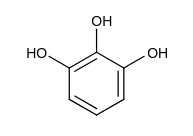
\includegraphics{smile-96f9a53603f88051f4036d2b758d1080ae1b15a6}\\
A) 1.2.3-trigidroksibenzol\\
B) 1.2.4-trigidroksibenzol\\
C) 1.3.5-trigidroksibenzol\\
D) 1.2.6-trigidroksibenzol
2. Quyidagi moddani sistematik nomenklatura bo'yicha nomlang.\\
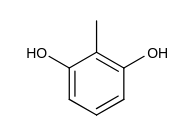
\includegraphics{smile-cff0ab9f74bf06a4ced7bdf12147de7fc9458903}\\
A) 1.2-digidroksi-3-metilbenzol\\
B) 1.3-digidroksi-4-metilbenzol\\
C) 1.3-digidroksi-2-metilbenzol\\
D) 1.2-digidroksi-2-metilbenzol\\
3. Quyidagi moddani sistematik nomenklatura bo'yicha nomlang.\\
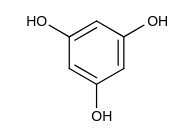
\includegraphics{smile-30c2a7fa3e4a236adc89c9e6298b6e3c89eba1c8}\\
A) 1.2.3-trigidroksibenzol\\
B) 1.2.4-trigidroksibenzol\\
C) 1.3.5-trigidroksibenzol\\
D) 1.2.6-trigidroksibenzol\\
4. Quyidagi moddani sistematik nomenklatura bo'yicha nomlang.\\
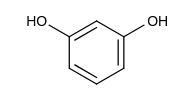
\includegraphics{smile-df4eb9172be3ecacb49269e48d5a02c66164f97b}\\
A) 1.3-digidroksibenzol\\
B) 1.2 -digidroksibenzol\\
C) 1.5 -digidroksibenzol\\
D) 1.4 -digidroksibenzol\\
5. Quyidagi moddani sistematik nomenklatura bo'yicha nomlang.\\
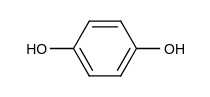
\includegraphics{smile-cd2cbef5676102a92391e7eb1c494695afc8cd70}\\
A) 1.3-digidroksibenzol\\
B) 1.2-digidroksibenzol\\
C) 1.5-digidroksibenzol\\
D) 1.4 -digidroksibenzol\\
6. Quyidagi moddani sistematik nomenklatura bo'yicha nomlang.\\
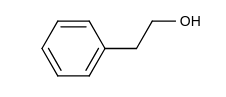
\includegraphics{smile-be35fec24ab189251980a3e7559aa7e7900d0310}\\
A) 2-feniletanol\\
B) 3-feniletanol\\
C) 1-feniletanol\\
D) 4-feniletanol\\
7. Quyidagi moddani sistematik nomenklatura bo'yicha nomlang.\\
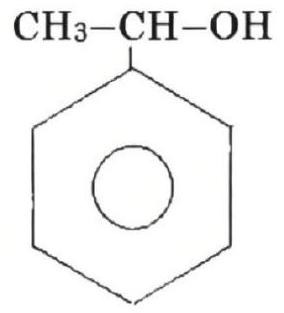
\includegraphics[max width=\textwidth, center]{2025_08_11_db5450af8b6ccbc40d9cg-04}\\
A) 2-feniletanol\\
B) 3-feniletanol\\
C) 1 -feniletanol\\
D) 4-feniletanol\\
8. Quyidagi moddani sistematik nomenklatura bo'yicha nomlang.\\
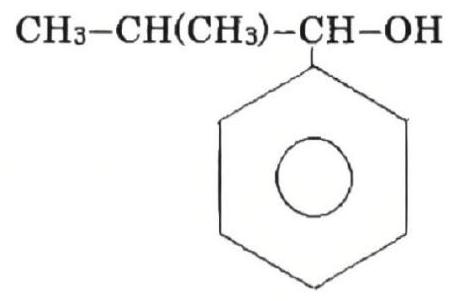
\includegraphics[max width=\textwidth, center]{2025_08_11_db5450af8b6ccbc40d9cg-04(1)}\\
A) 1-fenil-2-metilpropanol-1\\
B) 1-fenil-2-metilpropanol-2\\
C) 3-fenil-2-metilpropanol-1\\
D) 3 -fenil-2-metilpropanol-2\\
9. Quyidagi moddani sistematik nomenklatura bo'yicha nomlang.\\
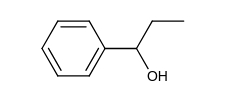
\includegraphics{smile-0917827eda5c3c9731d1a2d0c73424e47daf2bb4}\\
A) 1-fenilpropanol-3\\
B) 1-fenilpropanol-2\\
C) 1 -fenilpropanol-1\\
D) 2 -fenilpropanol- 1\\
10. Quyidagi moddani sistematik nomenklatura boyicha nomlang.\\
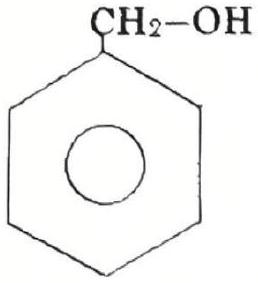
\includegraphics[max width=\textwidth, center]{2025_08_11_db5450af8b6ccbc40d9cg-05}\\
A) fenilbutanol\\
B) fenilpropanol\\
C) fenilmetanol\\
D) feniletanol
  \item 28.2 g fenol olish uchun talab etiladigan xlorbenzol va $20 \%$ li NaOH eritmasidan necha g dan kerak bo'ladi? (reaksiya unumi $50 \%$ )\\
A) $67,5 ; 120$\\
B) $67,5 ; 80$\\
C) $33,75 ; 120$\\
D) $135 ; 120$
  \item $9,4 \mathrm{~g}$ fenol olish uchun talab etiladigan xlorbenzol va $40 \%$ li NaOH eritmasidan necha g dan kerak bo'ladi? (reaksiya unumi $100 \%$ )\\
A) 11,$25 ; 16$\\
B) 11,$25 ; 8$\\
C) 11,$25 ; 15$\\
D) 11,$25 ; 10$
  \item $18,8 \mathrm{~g}$ fenol olish uchun talab etiladigan xlorbenzol va $50 \%$ li NaOH eritmasidan necha g dan kerak bo'ladi? (reaksiya unumi $80 \%$ )\\
A) 28,$125 ; 40$\\
B) 28,$125 ; 25$\\
C) 28,$125 ; 20$\\
D) 28,$125 ; 16$
  \item 94 g fenol olish uchun talab etiladigan xlorbenzol va $25 \%$ li NaOH eritmasidan necha g dan kerak bo'ladi? (reaksiya unumi $40 \%$ )\\
A) $281,25 ; 400$\\
B) $281,25: 200$\\
C) $112,5 ; 400$\\
D) $281,25 ; 250$
  \item $23,5 \mathrm{~g}$ fenol olish uchun talab etiladigan xlorbenzol va $40 \%$ li NaOH eritmasidan necha g dan kerak bo'ladi? (reaksiya unumi $100 \%$ )\\
A) $28,125 ; 25$\\
B) $28,125 ; 40$\\
C) $28,125 ; 50$\\
D) $56,25 ; 25$
  \item 47 g fenol olish uchun talab etiladigan xlorbenzol va $80 \%$ li NaOH eritmasidan necha g dan kerak bo'ladi? (reaksiya unumi $50 \%$ )\\
A) $122,5 ; 60$\\
B) $245 ;  50$\\
C) $122,5 ; 50$\\
D) $122,5 ; 40$
  \item $37,6 \mathrm{~g}$ fenol olish uchun talab etiladigan xlorbenzol va $50 \%$ li NaOH eritmasidan necha g dan kerak bo'ladi? (reaksiya unumi $50 \%$ )\\
A) $90 ; 32$\\
B) $90 ; 64$\\
C) $45 ; 64$\\
D) $80 ; 64$
  \item $75,2 \mathrm{~g}$ fenol olish uchun talab etiladigan xlorbenzol va $80 \%$ li NaOH eritmasidan necha g dan kerak bo'ladi?? (reaksiya unumi $50 \%$ )\\
A) $90 ; 80$\\
B) $180 ; 40$\\
C) $180 ; 120$\\
D) $180 ; 80$
  \item $56,4 \mathrm{~g}$ fenol olish uchun talab etiladigan xlorbenzol va $40 \%$ li NaOH eritmasidan necha g dan kerak bo'ladi? (reaksiya unumi $50 \%$ )\\
A) $67,5 ; 120$\\
B) $67,5 ; 80$\\
C) $33,75 ; 120$\\
D) $135 ; 120$
  \item $65,8 \mathrm{~g}$ fenol oli sh uchun talab etiladigan xlorbenzol va $80 \%$ li NaOH eritmasidan necha g dan kerak bo'ladi? (reaksiya unumi $100 \%$ )\\
A) $78,75 ; 70$\\
B) $78,75: 35$\\
C) $157,5 ; 35$\\
D) $78,75 ; 140$
  \item Asetilendan uch bosqichda fenol olinadi. 78 g asetilendan foydalanib necha g fenol olish mumkin?\\
A) 94\\
B) 47\\
C) 18,8\\
D) 188
  \item Asetilendan uch bosqichda fenol olinadi. 13 g asetilendan foydalanib necha g fenol olish mumkin?\\
A) 31,33\\
B) 47\\
C) 15,67\\
D) 18,8
  \item Asetilendan uch bosqichda fenol olinadi. 26 g asetilendan foydalanib necha g fenol olish mumkin?\\
A) 31,33\\
B) 47\\
C) 15,67\\
D) 18,8
  \item Asetilendan uch bosqichda fenol olinadi. 52 g asetilendan foydalanib necha g fenol olish mumkin?\\
A) 94,44\\
B) 62,67\\
C) 18,87\\
D) 46,67
  \item Asetilendan uch bosqichda fenol olinadi. $7,8 \mathrm{~g}$ asetilendan foydalanib necha g fenol olish mumkin?\\
A) 9,4\\
B) 4,7\\
C) 18,8\\
D) 7,8
  \item Asetilendan uch bosqichda fenol olinadi. 130 g asetilendan foydalanib necha g fenol olish mumkin?\\
A) 783,33\\
B) 156,67\\
C) 626,67\\
D) 313,33
  \item Asetilendan uch bosqichda fenol olinadi. 260 g asetilendan foydalanib necha g fenol olish mumkin?\\
A) 783,33\\
B) 156,67\\
C) 626,67\\
D) 313,33
  \item Asetilendan uch bosqichda fenol olinadi. 39 g asetilendan foydalanib necha g fenol olish mumkin?\\
A) 94\\
B) 47\\
C) 18,8\\
D) 188
  \item Asetilendan uch bosqichda fenol olinadi. 156 g asetilendan foydalanib necha g fenol olish mumkin?\\
A) 94\\
B) 47\\
C) 18,8\\
D) 188
  \item Asetilendan uch bosqichda fenol olinadi. $31,2 \mathrm{~g}$ asetilendan foydalanib necha g fenol olish mumkin?\\
A) 94\\
B) 37,6\\
C) 18,8\\
D) 47
  \item $0,05 \mathrm{~mol}$ fenolni bromlashda ( $2,4,6$ tribromfenol hosil bo'ladi) hosil bo'lgan gazsimon mahsulotni neytrallash uchun $12 \%$ li kaliy gidroksid eritmasidan qancha massa (g) sarflanadi?\\
A) 8,4\\
B) 70\\
C) 56\\
D) 16,8
  \item $0,1 \mathrm{~mol}$ fenolni bromlashda ( $2,4,6$ tribromfenol hosil bo'ladi) hosil bo'lgan gazsimon mahsulotni neytrallash uchun $24 \%$ li kaliy gidroksid eritmasidan qancha massa (g) sarflanadi?\\
A) 8,4\\
B) 70\\
C) 56\\
D) 16,8
  \item $0,5 \mathrm{~mol}$ fenolni bromlashda ( $2,4,6$ tribromfenol hosil bo'ladi) hosil bo'lgan gazsimon mahsulotni neytrallash uchun 56 \% li kaliy gidroksid eritmasidan qancha massa (g) sarflanadi?\\
A) 75\\
B) 140\\
C) 200\\
D) 150
  \item $0,04 \mathrm{~mol}$ fenolni bromlashda ( $2,4,6$ tribromfenol hosil bo'ladi) hosil bo'lgan gazsimon mahsulotni neytrallash uchun 40 \% li kaliy gidroksid eritmasidan qancha massa (g) sarflanadi?\\
A) 8,4\\
B) 70\\
C) 56\\
D) 16,8
  \item $0,1 \mathrm{~mol}$ fenolni bromlashda ( $2,4,6$ tribromfenol hosil bo'ladi) hosil bo'lgan gazsimon mahsulotni neytrallash uchun 11,2 \% li kaliy gidroksid eritmasidan qancha massa (g) sarflanadi?\\
A) 84\\
B) 56\\
C) 150\\
D) 250
  \item $0,2 \mathrm{~mol}$ fenolni bromlashda ( $2,4,6$ tribromfenol hosil bo'ladi) hosil bo'lgan gazsimon mahsulotni neytrallash uchun\\
$14 \%$ li kaliy gidroksid eritmasidan qancha massa (g) sarflanadi?\\
A) 240\\
B) 120\\
C) 56\\
D) 112
  \item $0,02 \mathrm{~mol}$ fenolni bromlashda ( $2,4,6$ tribromfenol hosil bo'ladi) hosil bo'lgan gazsimon mahsulotni neytrallash uchun 56 \% li kaliy gidroksid eritmasidan qancha massa $(\mathrm{g})$ sarflanadi?\\
A) 10\\
B) 8\\
C) 7\\
D) 6
  \item $0,08 \mathrm{~mol}$ fenolni bromlashda ( $2,4,6$ tribromfenol hosil bo'ladi) hosil bo'lgan gazsimon mahsulotni neytrallash uchun 28 \% li kaliy gidroksid eritmasidan qancha massa $(\mathrm{g})$ sarflanadi?\\
A) 84\\
B) 24\\
C) 48\\
D) 96
  \item $0,012 \mathrm{~mol}$ fenolni bromlashda ( $2,4,6$ tribromfenol hosil bo'ladi) hosil bo'lgan gazsimon mahsulotni neytrallash uchun $56 \%$ li kaliy gidroksid eritmasidan qancha massa (g) sarflanadi?\\
A) 8,4\\
B) 3,6\\
C) 5,6\\
D) 16,8
  \item $0,01 \mathrm{~mol}$ fenolni bromlashda ( $2,4,6$ tribromfenol hosil bo'ladi) hosil bo'lgan gazsimon mahsulotni neytrallash uchun $50 \%$ li kaliy gidroksid eritmasidan qancha massa (g) sarflanadi?\\
A) 8,4\\
B) 1,68\\
C) 5,6\\
D) 3,36
  \item Uch atomli fenol mo'l miqdordagi K metali bilan reaksiyaga kirishganda olingan moddaning molyar massasi 254 g/mol ga teng bo'lsa, dastlabki fenol formulasini toping.\\
A) $\mathrm{C}_{8} \mathrm{H}_{10} \mathrm{O}_{3}$\\
B) $\mathrm{C}_{7} \mathrm{H}_{8} \mathrm{O}_{3}$\\
C) $\mathrm{C}_{9} \mathrm{H}_{12} \mathrm{O}_{3}$\\
D) $\mathrm{C}_{9} \mathrm{H}_{11} \mathrm{O}_{2}$
42. Uch atomli fenol mo'l miqdordagi K metali bilan reaksiyaga kirishganda olingan moddaning molyar massasi 296 $\mathrm{g} / \mathrm{mol}$ ga teng bo'lsa, dastlabki fenol formulasini toping.\\
A) $\mathrm{C}_{10} \mathrm{H}_{13} \mathrm{O}_{3}$\\
B) $\mathrm{C}_{7} \mathrm{H}_{8} \mathrm{O}_{3}$\\
C) $\mathrm{C}_{9} \mathrm{H}_{12} \mathrm{O}_{3}$\\
D) $\mathrm{C}_{9} \mathrm{H}_{11} \mathrm{O}_{3}$\\
43. Uch atomli fenol mo'l miqdordagi K metali bilan reaksiyaga kirishganda olingan moddaning molyar massasi 282 $\mathrm{g} / \mathrm{mol}$ ga teng bo'lsa, dastlabki fenol formulasini toping.\\
A) $\mathrm{C}_{10} \mathrm{H}_{11} \mathrm{O}_{3}$\\
B) $\mathrm{C}_{7} \mathrm{H}_{8} \mathrm{O}_{3}$\\
C) $\mathrm{C}_{9} \mathrm{H}_{12} \mathrm{O}_{3}$\\
D) $\mathrm{C}_{9} \mathrm{H}_{9} \mathrm{O}_{3}$\\
44. Uch atomli fenol mo'l miqdordagi K metali bilan reaksiyaga kirishganda olingan moddaning molyar massasi 268 $\mathrm{g} / \mathrm{mol}$ ga teng bo'lsa, dastlabki fenol formulasini toping.\\
A) $\mathrm{C}_{8} \mathrm{H}_{10} \mathrm{O}_{3}$\\
B) $\mathrm{C}_{7} \mathrm{H}_{8} \mathrm{O}_{3}$\\
C) $\mathrm{C}_{9} \mathrm{H}_{12} \mathrm{O}_{3}$\\
D) $\mathrm{C}_{9} \mathrm{H}_{11} \mathrm{O}_{2}$\\
45. Uch atomli fenol mo'l miqdordagi K metali bilan reaksiyaga kirishganda olingan moddaning molyar massasi 324 g/mol ga teng bo'lsa, dastlabki fenol formulasini toping.\\
A) $\mathrm{C}_{8} \mathrm{H}_{10} \mathrm{O}_{3}$\\
B) $\mathrm{C}_{14} \mathrm{H}_{19} \mathrm{O}_{3}$\\
C) $\mathrm{C}_{12} \mathrm{H}_{18} \mathrm{O}_{3}$\\
D) $\mathrm{C}_{9} \mathrm{H}_{11} \mathrm{O}_{2}$\\
46. Uch atomli fenol mo'l miqdordagi K metali bilan reaksiyaga kirishganda olingan moddaning molyar massasi 352 $\mathrm{g} / \mathrm{mol}$ ga teng bo'lsa, dastlabki fenol formulasini toping.\\
A) $\mathrm{C}_{14} \mathrm{H}_{22} \mathrm{O}_{3}$\\
B) $\mathrm{C}_{8} \mathrm{H}_{10} \mathrm{O}_{3}$\\
C) $\mathrm{C}_{9} \mathrm{H}_{12} \mathrm{O}_{3}$\\
D) $\mathrm{C}_{9} \mathrm{H}_{11} \mathrm{O}_{2}$\\
47. Uch atomli fenol mo'l miqdordagi K metali bilan reaksiyaga kirishganda olingan moddaning molyar massasi 338 $\mathrm{g} / \mathrm{mol}$ ga teng bo'lsa, dastlabki fenol formulasini toping.\\
A) $\mathrm{C}_{12} \mathrm{H}_{18} \mathrm{O}_{3}$\\
B) $\mathrm{C}_{7} \mathrm{H}_{8} \mathrm{O}_{3}$\\
C) $\mathrm{C}_{15} \mathrm{H}_{24} \mathrm{O}_{3}$\\
D) $\mathrm{C}_{13} \mathrm{H}_{20} \mathrm{O}_{3}$\\
48. Uch atomli fenol mo'l miqdordagi K metali bilan reaksiyaga kirishganda olingan moddaning molyar massasi 380 g/mol ga teng bo'lsa, dastlabki fenol formulasini toping.\\
A) $\mathrm{C}_{16} \mathrm{H}_{26} \mathrm{O}_{3}$\\
B) $\mathrm{C}_{11} \mathrm{H}_{22} \mathrm{O}_{3}$\\
C) $\mathrm{C}_{9} \mathrm{H}_{1 \cdot} \mathrm{O}_{5}$\\
D) $\mathrm{C}_{15} \mathrm{H}_{24} \mathrm{O}_{3}$\\
49. Uch atomli fenol mo'l miqdordagi K metali bilan reaksiyaga kirishganda olingan moddaning molyar massasi 310\\
g/mol ga teng bo'lsa, dastlabki fenol formulasini toping.\\
A) $\mathrm{C}_{8} \mathrm{H}_{10} \mathrm{O}_{3}$\\
B) $\mathrm{C}_{11} \mathrm{H}_{16} \mathrm{O}_{3}$\\
C) $\mathrm{C}_{9} \mathrm{H}_{12} \mathrm{O}_{3}$\\
D) $\mathrm{C}_{9} \mathrm{H}_{11} \mathrm{O}_{2}$\\
50. Uch atomli fenol mo'l miqdordagi K metali bilan reaksiyaga kirishganda olingan moddaning molyar massasi 366 $\mathrm{g} / \mathrm{mol}$ ga teng bo'lsa, dastlabki fenol formulasini toping.\\
A) $\mathrm{C}_{16} \mathrm{H}_{26} \mathrm{O}_{3}$\\
B) $\mathrm{C}_{14} \mathrm{H}_{22} \mathrm{O}_{3}$\\
C) $\mathrm{C}_{9} \mathrm{H}_{12} \mathrm{O}_{3}$\\
D) $\mathrm{C}_{15} \mathrm{H}_{24} \mathrm{O}_{3}$
  \item $112,8 \mathrm{~g}$ fenolning bromli suv bilan reaksiyasida 2-bromfenol, 4-bromfenol va 2,4,6-tribromfenollar $1: 2: 3 \mathrm{~mol}$ nisbatda hosil bo'lsa, reaksiyaga sarflangan $8 \% \mathrm{li}$ bromli suv massasini (kg) toping.\\
A) 4,8\\
B) 3,2\\
C) 1,6\\
D) 6,4
  \item $56,4 \mathrm{~g}$ fenolning bromli suv bilan reaksiyasida 2-bromfenol, 4-bromfenol va 2,4,6-tribromfenollar $1: 2: 3 \mathrm{~mol}$ nisbatda hosil bo'lsa, reaksiyaga sarflangan 12 \% li bromli suv massasini (kg) toping.\\
A) 4,8\\
B) 3,2\\
C) 1,6\\
D) 6,4
  \item 188 g fenolning bromli suv bilan reaksiyasida 2-bromfenol, 4-bromfenol va 2,4,6-tribromfenollar $1: 2: 3 \mathrm{~mol}$ nisbatda hosil bo'lsa, reaksiyaga sarflangan 16 \% li bromli suv massasini (kg) toping.\\
A) 16\\
B) 12\\
C) 4\\
D) 8
  \item 94 g fenolning bromli suv bilan reaksiyasida 2-bromfenol, 4-bromfenol va $2,4,6$-tribromfenollar $1: 2: 3 \mathrm{~mol}$ nisbatda hosil bo'lsa, reaksiyaga sarflangan 6,4 \% li bromli suv massasini ( kg ) toping.\\
A) 3\\
B) 4\\
C) 6\\
D) 5
  \item $225,6 \mathrm{~g}$ fenolning bromli suv bilan reaksiyasida 2-bromfenol, 4-bromfenol va 2,4,6-tribromfenollar $1: 2: 3 \mathrm{~mol}$ nisbatda\\hosil bo'lsa, reaksiyaga sarflangan $4 \%$ li bromli suv massasini (kg) toping.\\
A) 4,8\\
B) 19,2\\
C) 9,6\\
D) 6,4
  \item $56,4 \mathrm{~g}$ fenolning bromli suv bilan reaksiyasida 2-bromfenol, 4-bromfenol va 2,4,6-tribromfenollar $1: 1: 2 \mathrm{~mol}$ nisbatda hosil bo'lsa, reaksiyaga sarflangan 3,2 \% li bromli suv massasini (kg) toping.\\
A) 3\\
B) 4\\
C) 6\\
D) 5
  \item 470 g fenolning bromli suv bilan reaksiyasida 2-bromfenol, 4-bromfenol va 2,4,6-tribromfenollar $1: 1: 2 \mathrm{~mol}$ nisbatda hosil bo'lsa, reaksiyaga sarflangan $16 \%$ li bromli suv massasini (kg) toping.\\
A) 10\\
B) 6\\
C) 9\\
D) 6
  \item 47 g fenolning bromli suv bilan reaksiyasida 2-bromfenol, 4-bromfenol va 2,4,6-tribromfenollar $1: 1: 2 \mathrm{~mol}$ nisbatda hosil bo'lsa, reaksiyaga sarflangan $3,2 \% \mathrm{li}$ bromli suv massasini (kg) toping.\\
A) 3\\
B) 4\\
C) 6\\
D) 5
  \item $18,8 \mathrm{~g}$ fenolning bromli suv bilan reaksiyasida 2-bromfenol, 4-bromfenol va 2,4,6-tribromfenollar $1: 1: 2 \mathrm{~mol}$ nisbatda hosil bo'lsa, reaksiyaga sarflangan $8 \%$ li bromli suv massasini (kg) toping.\\
A) 1,2\\
B) 0,8\\
C) 1,6\\
D) 0,64
  \item $112,8 \mathrm{~g}$ fenolning bromli suv bilan reaksiyasida 2-bromfenol, 4-bromfenol va 2,4,6-tribromfenollar $1: 1: 2$ mol nisbatda hosil bo'lsa, reaksiyaga sarflangan $40 \%$ li bromli suv massasini (kg) toping.\\
A) 0,48\\
B) 0,96\\
C) 1,6\\
D) 0,64
  \item Etanol va fenoldan iborat 140 g aralashma mo'l miqdordagi kaliy metali bilan reaksiyasi natijasida \href{http://n.sh}{n.sh} da o'lchangan 22,4 litr gaz ajralgan bo'lsa, aralashmadagi fenol massasini (g) toping.\\
A) 94\\
B) 47\\
C) 18,8\\
D) 9,4
  \item Etanol va fenoldan iborat $37,4 \mathrm{~g}$ aralashma mo'l miqdordagi kaliy metali bilan reaksiyasi natijasida \href{http://n.sh}{n.sh} da o'lchangan 5,6 litr gaz ajralgan bo'lsa, aralashmadagi fenol massasini (g) toping.\\
A) 18,8\\
B) 4.7\\
C) 28,2\\
D) 9,4
  \item Etanol va fenoldan iborat $37,2 \mathrm{~g}$ aralashma mo'l miqdordagi kaliy metali bilan reaksiyasi natijasida \href{http://n.sh}{n.sh} da o'lchangan 6,72 litr gaz ajralgan bo'lsa, aralashmadagi fenol massasini (g) toping.\\
A) 94\\
B) 47\\
C) 18,8\\
D) 9,4
  \item Metanol va fenoldan iborat 22 g aralashma mo'l miqdordagi kaliy metali bilan reaksiyasi natijasida \href{http://n.sh}{n.sh} da o'lchangan 3,36 litr gaz ajralgan bo'lsa, aralashmadagi metanol massasini (g) toping.\\
A) 6,4\\
B) 3,2\\
C) 9,6\\
D) 12,8
  \item Metanol va fenoldan iborat 22 g aralashma mo'l miqdordagi kaliy metali bilan reaksiyasi natijasida \href{http://n.sh}{n.sh} da o'lchangan 3,36 litr gaz ajralgan bo'lsa, aralashmadagi metanol massasini (g) toping.\\
A) 6,4\\
B) 3,2\\
C) 9,6\\
D) 12,8
  \item Propanol va fenoldan iborat $83,8 \mathrm{~g}$ aralashma mo'l miqdordagi kaliy metali bilan reaksiyasi natijasida \href{http://n.sh}{n.sh} da o'lchangan 11,2 litr gaz ajralgan bo'lsa, aralashmadagi fenol massasini (g) toping.\\
A) 32,9\\
B) 65,8\\
C) 18,8\\
D) 9,4
  \item Propanol va fenoldan iborat $30,8 \mathrm{~g}$ aralashma mo'l miqdordagi kaliy metali bilan reaksiyasi natijasida \href{http://n.sh}{n.sh} da o'lchangan 4,48 litr gaz ajralgan bo'lsa, aralashmadagi fenol massasini (g) toping.\\
A) 32,9\\
B) 65,8\\
C) 18,8\\
D) 9,4
  \item Butanol va fenoldan iborat 45 g aralashma mo'l miqdordagi kaliy metali bilan reaksiyasi natijasida \href{http://n.sh}{n.sh} da\\
o'lchangan 5,6 litr gaz ajralgan bo'lsa, aralashmadagi butanol massasini (g) toping.\\
A) 7,4\\
B) 14,8\\
C) 11,1\\
D) 22,2
  \item Butanol va fenoldan iborat $50,4 \mathrm{~g}$ aralashma mo'l miqdordagi kaliy metali bilan reaksiyasi natijasida \href{http://n.sh}{n.sh} da o'lchangan 6.72 litr gaz ajralgan bo'lsa, aralashmadagi butanol massasini (g) toping.\\
A) 7,4\\
B) 14,8\\
C) 11,1\\
D) 22,2
  \item Etanol va fenoldan iborat $65,2 \mathrm{~g}$ aralashma mo'l miqdordagi kaliy metali bilan reaksiyasi natijasida \href{http://n.sh}{n.sh} da o'lchangan 11,2 litr gaz ajralgan bo'lsa, aralashmadagi fenol massasini (g) toping.\\
A) 18,8\\
B) 47\\
C) 37,6\\
D) 9,4
  \item $0,5 \mathrm{~mol}$ noma'lum bir atomli fenol tarkibidagi neytronlar sonicha neytron 50 g $\mathrm{CaCO}_{3}$ tarkibida bo'lsa, noma'lum fenolni aniqlang.\\
A) $\mathrm{C}_{7} \mathrm{H}_{8} \mathrm{O}$\\
B) $\mathrm{C}_{8} \mathrm{H}_{10} \mathrm{O}$\\
C) $\mathrm{C}_{9} \mathrm{H}_{12} \mathrm{O}$\\
D) $\mathrm{C}_{10} \mathrm{H}_{14} \mathrm{O}$
72. $0,6 \mathrm{~mol}$ noma'lum bir atomli fenol tarkibidagi neytronlar sonicha neytron $67,2 \mathrm{~g} \mathrm{MgSO}_{4}$ tarkibida bo'lsa, noma'lum fenolni aniqlang.\\
A) $\mathrm{C}_{7} \mathrm{H}_{8} \mathrm{O}$\\
B) $\mathrm{C}_{8} \mathrm{H}_{10} \mathrm{O}$\\
C) $\mathrm{C}_{9} \mathrm{H}_{12} \mathrm{O}$\\
D) $\mathrm{C}_{10} \mathrm{H}_{14} \mathrm{O}$\\
73. $0,4 \mathrm{~mol}$ noma'lum bir atomli fenol tarkibidagi neytronlar sonicha neytron $54,4 \mathrm{~g}$ HF tarkibida bo'lsa, noma'lum fenolni aniqlang.\\
A) $\mathrm{C}_{7} \mathrm{H}_{8} \mathrm{O}$\\
B) $\mathrm{C}_{8} \mathrm{H}_{10} \mathrm{O}$\\
C) $\mathrm{C}_{9} \mathrm{H}_{12} \mathrm{O}$\\
D) $\mathrm{C}_{10} \mathrm{H}_{14} \mathrm{O}$\\
74. $0,3 \mathrm{~mol}$ noma'lum bir atomli fenol tarkibidagi neytronlar sonicha neytron 30 g $\mathrm{N}_{2} \mathrm{O}$ tarkibida bo'lsa. noma'lum fenolni aniqlang.\\
A) $\mathrm{C}_{7} \mathrm{H}_{4} \mathrm{O}$\\
B) $\mathrm{C}_{8} \mathrm{H}_{10} \mathrm{O}$\\
C) $\mathrm{C}_{9} \mathrm{H}_{12} \mathrm{O}$\\
D) $\mathrm{C}_{10} \mathrm{H}_{14} \mathrm{O}$\\
75. $0,1 \mathrm{~mol}$ noma'lum bir atomli fenol tarkibidagi neytronlar sonicha neytron $12,4 \mathrm{~g} \mathrm{CO}_{2}$ tarkibida bo'lsa, noma'lum fenolni aniqlang.\\
A) $\mathrm{C}_{7} \mathrm{H}_{8} \mathrm{O}$\\
B) $\mathrm{C}_{8} \mathrm{H}_{10} \mathrm{O}$\\
C) $\mathrm{C}_{9} \mathrm{H}_{12} \mathrm{O}$\\
D) $\mathrm{C}_{10} \mathrm{H}_{14} \mathrm{O}$\\
76. $0,4 \mathrm{~mol}$ noma'lum bir atomli fenol tarkibidagi neytronlar sonicha neytron $44,8 \mathrm{~g} \mathrm{NO}$ tarkibida bo'lsa, noma'lum fenolni aniqlang.\\
A) $\mathrm{C}_{7} \mathrm{H}_{8} \mathrm{O}$\\
B) $\mathrm{C}_{8} \mathrm{H}_{10} \mathrm{O}$\\
C) $\mathrm{C}_{9} \mathrm{H}_{12} \mathrm{O}$\\
D) $\mathrm{C}_{10} \mathrm{H}_{14} \mathrm{O}$\\
77. $0,2 \mathrm{~mol}$ noma'lum bir atomli fenol tarkibidagi neytronlar sonicha neytron 20 g $\mathrm{SiO}_{2}$ tarkibida bo'lsa, noma'lum fenolni aniqlang.\\
A) $\mathrm{C}_{7} \mathrm{H}_{8} \mathrm{O}$\\
B) $\mathrm{C}_{8} \mathrm{H}_{10} \mathrm{O}$\\
C) $\mathrm{C}_{9} \mathrm{H}_{12} \mathrm{O}$\\
D) $\mathrm{C}_{10} \mathrm{H}_{14} \mathrm{O}$\\
78. $0,2 \mathrm{~mol}$ noma'lum bir atomli fenol tarkibidagi neytronlar sonicha neytron $27,2 \mathrm{~g} \mathrm{~N}_{2} \mathrm{O}_{5}$ tarkibida bo'lsa, noma'lum fenolni aniqlang.\\
A) $\mathrm{C}_{7} \mathrm{H}_{8} \mathrm{O}$\\
B) $\mathrm{C}_{8} \mathrm{H}_{10} \mathrm{O}$\\
C) $\mathrm{C}_{9} \mathrm{H}_{12} \mathrm{O}$\\
D) $\mathrm{C}_{10} \mathrm{H}_{14} \mathrm{O}$\\
79. $0,8 \mathrm{~mol}$ noma'lum bir atomli fenol tarkibidagi neytronlar sonicha neytron 80 g $\mathrm{MgCO}_{3}$ tarkibida bo'lsa, noma'lum fenolni aniqlang.\\
A) $\mathrm{C}_{7} \mathrm{H}_{8} \mathrm{O}$\\
B) $\mathrm{C}_{8} \mathrm{H}_{10} \mathrm{O}$\\
C) $\mathrm{C}_{9} \mathrm{H}_{12} \mathrm{O}$\\
D) $\mathrm{C}_{10} \mathrm{H}_{14} \mathrm{O}$\\
80. $0,6 \mathrm{~mol}$ noma'lum bir atomli fenol tarkibidagi neytronlar sonicha neytron $74,4 \mathrm{~g} \mathrm{~N}_{2} \mathrm{O}_{3}$ tarkibida bo'lsa, noma'lum fenolni aniqlang.\\
A) $\mathrm{C}_{7} \mathrm{H}_{8} \mathrm{O}$\\
B) $\mathrm{C}_{8} \mathrm{H}_{10} \mathrm{O}$\\
C) $\mathrm{C}_{9} \mathrm{H}_{12} \mathrm{O}$\\
D) $\mathrm{C}_{10} \mathrm{H}_{14} \mathrm{O}$\\
81. Etanol va fenol aralashmasi natriy metali bilan to'liq reaksiyaga kirishganda \href{http://n.sh}{n.sh} da o'lchangan 4,48 litr gaz ajraldi. Shu aralashma $50 \mathrm{~g} 16 \%$ li NaOH bilan to'liq reaksiyaga kirishsa, dastlabki aralashmadagi spirt massasini (g) aniqlang.\\
A) 9,2\\
B) 4,6\\
C) 18,4\\
D) 36,8
  \item Etanol va fenol aralashmasi natriy metali bilan to'liq reaksiyaga kirishganda \href{http://n.sh}{n.sh} da o'lchangan 8,96 litr gaz ajraldi. Shu aralashma $50 \mathrm{~g} 32 \%$ li NaOH bilan to'liq reaksiyaga kirishsa, dastlabki aralashmadagi spirt massasini (g) aniqlang.\\
A) 9,2\\
B) 4,6\\
C) 18,4\\
D) 36,8
  \item Etanol va fenol aralashmasi natriy metali bilan to'liq reaksiyaga kirishganda \href{http://n.sh}{n.sh} da o'lchangan 5,6 litr gaz ajraldi. Shu aralashma $50 \mathrm{~g} 16 \%$ li NaOH bilan to'liq reaksiyaga kirishsa, dastlabki aralashmadagi spirt massasini (g) aniqlang.\\
A) 23\\
B) 13,8\\
C) 11,5\\
D) 36,8
  \item Metanol va fenol aralashmasi natriy metali bilan to'liq reaksiyaga kirishganda \href{http://n.sh}{n.sh} da o'lchangan 5,6 litr gaz ajraldi. Shu aralashma $50 \mathrm{~g} 24 \%$ li NaOH bilan to'liq reaksiyaga kirishsa, dastlabki\\
aralashmadagi spirt massasini (g) aniqlang.\\
A) 12,8\\
B) 9.6\\
C) 3,2\\
D) 6,4
  \item Metanol va fenol aralashmasi natriy metali bilan to'liq reaksiyaga kirishganda \href{http://n.sh}{n.sh} da o'lchangan 6,72 litr gaz ajraldi. Shu aralashma $50 \mathrm{~g} 16 \%$ li NaOH bilan to'liq reaksiyaga kirishsa, dastlabki aralashmadagi spirt massasini (g) aniqlang.\\
A) 12,8\\
B) 9,6\\
C) 3,2\\
D) 6,4
  \item Metanol va fenol aralashmasi natriy metali bilan to'liq reaksiyaga kirishganda $\mathrm{n} . \mathrm{sh}$ da o'lchangan 2,24 litr gaz ajraldi. Shu aralashma $50 \mathrm{~g} 8 \%$ li NaOH bilan to'liq reaksiyaga kirishsa, dastlabki aralashmadagi spirt massasini (g) aniqlang.\\
A) 12,8\\
B) 9,6\\
C) 3,2\\
D) 6,4
  \item Metanol va fenol aralashmasi natriy metali bilan to'liq reaksiyaga kirishganda \href{http://n.sh}{n.sh} da o'lchangan 6,72 litr gaz ajraldi. Shu aralashma $50 \mathrm{~g} 24 \%$ li NaOH bilan to'liq reaksiyaga kirishsa, dastlabki aralashmadagi spirt massasini (g) aniqlang.\\
A) 9,6\\
B) 8\\
C) 1,6\\
D) 16
  \item Butanol va fenol aralashmasi natriy metali bilan to'liq reaksiyaga kirishganda \href{http://n.sh}{n.sh} da o'lchangan 4,48 litr gaz ajraldi. Shu aralashma $50 \mathrm{~g} 16 \%$ li NaOH bilan to'liq reaksiyaga kirishsa, dastlabki aralashmadagi spirt massasini (g) aniqlang.\\
A) 14,8\\
B) 44,4\\
C) 7,4\\
D) 3,7
  \item Butanol va fenol aralashmasi natriy metali bilan to'liq reaksiyaga kirishganda \href{http://n.sh}{n.sh} da o'lchangan 11,2 litr gaz ajraldi. Shu aralashma $50 \mathrm{~g} 32 \%$ li NaOH bilan to'liq reaksiyaga kirishsa, dastlabki aralashmadagi spirt massasini (g) aniqlang.\\
A) 14,8\\
B) 44,4\\
C) 7,4\\
D) 3,7
  \item Butanol va fenol aralashmasi natriy metali bilan to'liq reaksiyaga kirishganda \href{http://n.sh}{n.sh} da o'lchangan 5,6 litr gaz ajraldi. Shu\\
aralashma $50 \mathrm{~g} 32 \%$ li NaOH bilan to'liq reaksiyaga kirishsa, dastlabki aralashmadagi spirt massasini (g) aniqlang.\\
A) 14,8\\
B) 44,4\\
C) 7,4\\
D) 3,7
  \item $18,8 \mathrm{~g}$ fenol saqlagan suvli eritmaga $5,6 \mathrm{~g} \mathrm{KOH}$ saqlagan suvli eritma qo'shildi. Reaksiya natijasida ortib qolgan fenol massasini (g) toping.\\
A) 9,4\\
B) 18,8\\
C) 4,7\\
D) 28,2
  \item $37,6 \mathrm{~g}$ fenol saqlagan suvli eritmaga $11,2 \mathrm{~g} \mathrm{KOH}$ saqlagan suvli eritma qo'shildi. Reaksiya natijasida ortib qolgan fenol massasini (g) toping.\\
A) 9,4\\
B) 18,8\\
C) 4,7\\
D) 28,2
  \item $28,2 \mathrm{~g}$ fenol saqlagan suvli eritmaga $2,8 \mathrm{~g} \mathrm{KOH}$ saqlagan suvli eritma qo'shildi. Reaksiya natijasida ortib qolgan fenol massasini (g) toping.\\
A) 9,4\\
B) 11,75\\
C) 4,7\\
D) 23,5
  \item $14,1 \mathrm{~g}$ fenol saqlagan suvli eritmaga $2,8 \mathrm{~g} \mathrm{KOH}$ saqlagan suvli eritma qo'shildi. Reaksiya natijasida ortib qolgan fenol massasini (g) toping.\\
A) 9,4\\
B) 18,8\\
C) 4,7\\
D) 28,2
  \item $56,4 \mathrm{~g}$ fenol saqlagan suvli eritmaga $22,4 \mathrm{~g} \mathrm{KOH}$ saqlagan suvli eritma qo'shildi. Reaksiya natijasida ortib qolgan fenol massasini (g) toping.\\
A) 9,4\\
B) 18,8\\
C) 4,7\\
D) 28,2
  \item $28,2 \mathrm{~g}$ fenol saqlagan suvli eritmaga 6 g NaOH saqlagan suvli eritma qo'shildi. Reaksiya natijasida ortib qolgan fenol massasini (g) toping.\\
A) 18,8\\
B) 11,75\\
C) 14,1\\
D) 28,2
  \item $18,8 \mathrm{~g}$ fenol saqlagan suvli eritmaga 4 g NaOH saqlagan suvli eritma qo'shildi. Reaksiya natijasida ortib qolgan fenol massasini (g) toping.\\
A) 9,4\\
B) 18,8\\
C) 4,7\\
D) 28,2
  \item $37,6 \mathrm{~g}$ fenol saqlagan suvli eritmaga 4 g NaOH saqlagan suvli eritma qo'shildi. Reaksiya natijasida ortib qolgan fenol massasini (g) toping.\\
A) 9,4\\
B) 18,8\\
C) 4,7\\
D) 28,2
  \item 23.5 g fenol saqlagan suvli eritmaga 6 $\mathrm{g} \mathrm{NaOH} \mathrm{saqlagan} \mathrm{suvli} \mathrm{eritma} \mathrm{qo'shildi}$. Reaksiya natijasida ortib qolgan fenol massasini (g) toping.\\
A) 9,4\\
B) 18,8\\
C) 4,7\\
D) 28,2
  \item $14,1 \mathrm{~g}$ fenol saqlagan suvli eritmaga 4 g NaOH saqlagan suvli eritma qo'shildi. Reaksiya natijasida ortib qolgan fenol massasini (g) toping.\\
A) 9,4\\
B) 18,8\\
C) 4,7\\
D) 28,2
  \item Quyidagi oddiy efirni ratsional nomenkilatura bo'yicha nomlang. $\mathrm{CH}_{3}-\mathrm{O}-\mathrm{C}_{2} \mathrm{H}_{5}$\\
A) metil-etilefir\\
B) dimetilefir\\
C) etil-izopropilefir\\
D) dietilefir
  \item Quyidagi oddiy efirni ratsional nomenkilatura bo'yicha nomlang. $\mathrm{C}_{2} \mathrm{H}_{5}-\mathrm{O}-\mathrm{C}_{2} \mathrm{H}_{5}$\\
A) metil-etilefir\\
B) dimetilefir\\
C) etil-izopropilefir\\
D) dietilefir
  \item Quyidagi oddiy efirni ratsional nomenkilatura bo'yicha nomlang. $\mathrm{CH}_{3}-\mathrm{O}-\mathrm{CH}_{3}$\\
A) metil-etilefir\\
B) dimetilefir\\
C) etil-izopropilefir\\
D) dietilefir
  \item Quyidagi oddiy efirni ratsional nomenkilatura bo'yicha nomlang. $\mathrm{CH}_{3}-\mathrm{O}-\mathrm{CH}\left(\mathrm{CH}_{3}\right)_{2}$\\
A) metil-izopropilefir\\
B) metil-propilefir\\
C) etil-izopropilefir\\
D) metil-izobutilefir
  \item Quyidagi oddiy efirni ratsional nomenkilatura bo'yicha nomlang. $\mathrm{C}_{3} \mathrm{H}_{7}-\mathrm{O}-\mathrm{C}_{2} \mathrm{H}_{5}$\\
A) metil-izopropilefir\\
B) etil-izopropilefir\\
C) metil-propilefir\\
D) etil-propilefir
  \item Quyidagi oddiy efirni ratsional nomenkilatura bo'yicha nomlang. $\mathrm{CH}_{3}-\mathrm{O}-\mathrm{C}_{4} \mathrm{H}_{9}$\\
A) etil-butilefir\\
B) metil-izobutilefir\\
C) metil-butilefir\\
D) etil-izobutilefir
  \item Quyidagi oddiy efirni ratsional nomenkilatura bo'yicha nomlang.\\
$\mathrm{CH}_{3} \mathrm{CH}\left(\mathrm{CH}_{3}\right) \mathrm{CH}_{2}-\mathrm{O}-\mathrm{C}_{2} \mathrm{H}_{5}$\\
A) etil-butilefir\\
B) metil-izobutilefir\\
C) metil-butilefir\\
D) etil-izobutilefir
  \item Quyidagi oddiy efirni ratsional nomenkilatura bo'yicha nomlang.\\
$\mathrm{CH}_{3} \mathrm{CH}\left(\mathrm{CH}_{3}\right) \mathrm{CH}_{2}-\mathrm{O}-\mathrm{CH}\left(\mathrm{CH}_{3}\right)_{2}$\\
A) propil-izobutilefir\\
B) izopropil-izobutilefir\\
C) izopropil-butilefir\\
D) propil-butilefir
  \item Quyidagi oddiy efirni ratsional nomenkilatura bo'yicha nomlang. $\mathrm{C}_{3} \mathrm{H}_{7}-\mathrm{O}-\mathrm{C}_{3} \mathrm{H}_{7}$\\
A) metil-etilefir\\
B) dimetilefir\\
C) etil-izopropilefir\\
D) dipropilefir
  \item Quyidagi oddiy efirni ratsional nomenkilatura bo'yicha nomlang. $\mathrm{C}_{4} \mathrm{H}_{9}-\mathrm{O}-\mathrm{C}_{4} \mathrm{H}_{9}$\\
A) metil-etilefir\\
B) dibutilefir\\
C) etil-izopropilefir\\
D) dietilefir
11. Quyidagi oddiy efirni sistematik nomenkilatura bo'yicha nomlang. $\mathrm{CH}_{3}-\mathrm{O}-\mathrm{C}_{2} \mathrm{H}_{5}$\\
A) etoksietan\\
B) metoksimetan\\
C) metoksietan\\
D) 2 -metoksipropan\\
12. Quyidagi oddiy efirni sistematik nomenkilatura bo'yicha nomlang.\\
$\mathrm{C}_{2} \mathrm{H}_{5}-\mathrm{O}-\mathrm{C}_{2} \mathrm{H}_{5}$\\
A) etoksietan\\
B) metoksimetan\\
C) metoksietan\\
D) 2-metoksipropan\\
13. Quyidagi oddiy efirni sistematik nomenkilatura bo'yicha nomlang. $\mathrm{CH}_{3}-\mathrm{O}-\mathrm{CH}_{3}$\\
A) etoksietan\\
B) metoksimetan\\
C) metoksietan\\
D) 2 -metoksipropan\\
14. Quyidagi oddiy efirni sistematik nomenkilatura bo'yicha nomlang. $\mathrm{CH}_{3}-\mathrm{O}-\mathrm{CH}\left(\mathrm{CH}_{3}\right)_{2}$\\
A) etoksietan\\
B) metoksimetan\\
C) metoksietan\\
D) 2 -metoksipropan\\
15. Quyidagi oddiy efirni sistematik nomenkilatura bo'yicha nomlang.\\
$\mathrm{C}_{3} \mathrm{H}_{7}-\mathrm{O}-\mathrm{C}_{2} \mathrm{H}_{5}$\\
A) metoksibutan\\
B) 1-izopropoksi-2-metilpropan\\
C) 1-etoksi-2-metilpropan\\
D) etoksipropan\\
16. Quyidagi oddiy efirni sistematik nomenkiIatura bo'yicha nomlang.\\
$\mathrm{CH}_{3}-\mathrm{O}-\mathrm{C}_{4} \mathrm{H}_{9}$\\
A) metoksibutan\\
B) 1-izopropoksi-2-metilpropan\\
C) 1-etoksi-2-metilpropan\\
D) etoksipropan\\
17. Quyidagi oddiy efirni sistematik nomenkilatura bo'yicha nomlang.\\
$\mathrm{CH}_{3} \mathrm{CH}\left(\mathrm{CH}_{3}\right) \mathrm{CH}_{2}-\mathrm{O}-\mathrm{C}_{2} \mathrm{H}_{5}$\\
A) metoksibutan\\
B) 1-izopropoksi-2-metilpropan\\
C) 1-etoksi-2-metilpropan\\
D) etoksipropan\\
18. Quyidagi oddiy efirni sistematik nomenkilatura bo'yicha nomlang.\\
$\mathrm{CH}_{3} \mathrm{CH}\left(\mathrm{CH}_{3}\right) \mathrm{CH}_{2}-\mathrm{O}-\mathrm{CH}\left(\mathrm{CH}_{3}\right)_{2}$\\
A) metoksibutan\\
B) 1-izopropoksi-2-metilpropan\\
C) 1-etoksi-2-metilpropan\\
D) etoksipropan\\
19. Quyidagi oddiy efirni sistematik nomenkilatura bo'yicha nomlang.\\
$\mathrm{C}_{3} \mathrm{H}_{7}-\mathrm{O}-\mathrm{C}_{3} \mathrm{H}_{7}$\\
A) propoksipropan\\
B) metoksimetan\\
C) metoksietan\\
D) butoksibutan\\
20. Quyidagi oddiy efirni sistematik nomenkilatura bo'yicha nomlang. $\mathrm{C}_{4} \mathrm{H}_{9}-\mathrm{O}-\mathrm{C}_{4} \mathrm{H}_{9}$\\
A) propoksipropan\\
B) metoksimetan\\
C) metoksietan\\
D) butoksibutan
  \item Metil va etil spirtlari aralashmasi katalizator ishtirokida reaksiyaga kirishganda quyidagi oddiy efirlardan qaysi biri hosil bo'lmaydi?\\
A) propoksipropan\\
B) metoksimetan\\
C) metoksietan\\
D) etoksietan
22. Propil va etil spirtlari aralashmasi katalizator ishtirokida reaksiyaga kirishganda quyidagi oddiy efirlardan qaysi biri hosil bo'lmaydi?\\
A) propoksipropan\\
B) etoksietan\\
C) metoksietan\\
D) etoksipropan\\
23. Metil va butil spirtlari aralashmasi katalizator ishtirokida reaksiyaga kirishganda quyidagi oddiy efirlardan qaysi biri hosil bo'lmaydi?\\
A) butoksibutan\\
B) metoksipropan\\
C) metoksimetan\\
D) metoksibutan\\
24. Propil va butil spirtlari aralashmasi katalizator ishtirokida reaksiyaga kirishganda quyidagi oddiy efirlardan qaysi biri hosil bo'lmaydi?\\
A) propoksibutan\\
B) etoksibutan\\
C) propoksipropan\\
D) butoksibutan\\
25. Butil va etil spirtlari aralashmasi katalizator ishtirokida reaksiyaga kirishganda quyidagi oddiy efirlardan qaysi biri hosil bo'lmaydi?\\
A) propoksibutan\\
B) etoksibutan\\
C) etoksietan\\
D) butoksibutan\\
26. Metil va propil spirtlari aralashmasi katalizator ishtirokida reaksiyaga kirishganda quyidagi oddiy efirlardan qaysi biri hosil bo'lmaydi?\\
A) propoksipropan\\
B) metoksietan\\
C) metoksimetan\\
D) metoksipropan\\
27. Butil va pentil spirtlari aralashmasi katalizator ishtirokida reaksiyaga kirishganda quyidagi oddiy efirlardan qaysi biri hosil bo'lmaydi?\\
A) butoksipentan\\
B) metoksietan\\
C) butoksibutan\\
D) pentoksipentan\\
28. Metil va pentil spirtlari aralashmasi katalizator ishtirokida reaksiyaga kirishganda quyidagi oddiy efirlardan qaysi biri hosil bo'lmaydi?\\
A) propoksipentan\\
B) metoksimetan\\
C) metoksipentan\\
D) pentoksipentan\\
29. Propil va pentil spirtlari aralashmasi katalizator ishtirokida reaksiyaga kirishganda quyidagi oddiy efirlardan qaysi biri hosil bo'lmaydi?\\
A) propoksipentan\\
B) pentoksipentan\\
C) propoksipropan\\
D) etoksietan\\
30. Pentil va etil spirtlari aralashmasi katalizator ishtirokida reaksiyaga kirishganda quyidagi oddiy efirlardan qaysi biri hosil bo'lmaydi?\\
A) propoksipentan\\
B) etoksietan\\
C) etoksipentan\\
D) propoksipent\\
31. Etil va metil spirtlari reaksiyasi natijasida mol nisbati mos ravishda $1 ; 2 ; 1$ nisbatda dimetil, metiletil, va dietilefirlar aralashmasi olindi. Agar reaksiya uchun sarflangan etanol massasi $18,4 \mathrm{~g}$ bo'lsa, hosil bo'lgan metiletilefir massasini (g) hisoblang.\\
A) 12\\
B) 24\\
C) 36\\
D) 48
  \item Etil va metil spirtlari reaksiyasi natijasida mol nisbati mos ravishda $1 ; 2 ; 1$ nisbatda dimetil, metiletil, va dietilefirlar aralashmasi olindi. Agar reaksiya uchun sarflangan etanol massasi 46 g bo'lsa, hosil bo'lgan dietilefir massasini (g) hisoblang.\\
A) 37\\
B) 7,4\\
C) 18,5\\
D) 74
  \item Etil va metil spirtlari reaksiyasi natijasida mol nisbati mos ravishda $1 ; 2 ; 1$ nisbatda dimetil, metiletil, va dietilefirlar aralashmasi olindi. Agar reaksiya uchun sarflangan etanol massasi 92 g bo'lsa, hosil bo'lgan dimetilefir massasini (g) hisoblang.\\
A) 9,2\\
B) 11,5\\
C) 46\\
D) 23
  \item Etil va metil spirtlari reaksiyasi natijasida mol nisbati mos ravishda $1 ; 1 ; 1$ nisbatda dimetil, metiletil, va dietilefirlar aralashmasi olindi. Agar reaksiya uchun sarflangan metanol massasi 32 g bo'lsa, hosil bo'lgan metiletilefir massasini (g) hisoblang.\\
A) 12\\
B) 20\\
C) 40\\
D) 60
  \item Etil va metil spirtlari reaksiyasi natijasida mol nisbati mos ravishda $1 ; 1 ; 1$ nisbatda dimetil, metiletil, va dietilefirlar aralashmasi olindi. Agar reaksiya uchun sarflangan metanol massasi 48 g bo'lsa,\\
hosil bo'lgan dietilefir massasini (g) hisoblang.\\
A) 7,4\\
B) 14,8\\
C) 37\\
D) 74
  \item Etil va metil spirtlari reaksiyasi natijasida mol nisbati mos ravishda $1 ; 1 ; 1$ nisbatda dimetil, metiletil, va dietilefirlar aralashmasi olindi. Agar reaksiya uchun sarflangan metanol massasi 96 g bo'lsa, hosil bo'lgan dimetilefir massasini (g) hisoblang.\\
A) 46\\
B) 23\\
C) 92\\
D) 18,4
  \item Etil va metil spirtlari reaksiyasi natijasida mol nisbati mos ravishda $1 ; 1 ; 1$ nisbatda dimetil, metiletil, va dietilefirlar aralashmasi olindi. Agar reaksiya uchun sarflangan metanol massasi $12,8 \mathrm{~g}$ bo'lsa, hosil bo'lgan metiletilefir massasini (g) hisoblang.\\
A) 32\\
B) 24\\
C) 16\\
D) 8
  \item Etil va metil spirtlari reaksiyasi natijasida mol nisbati mos ravishda $1 ; 2 ; 2$ nisbatda dimetil, metiletil, va dietilefirlar aralashmasi olindi. Agar reaksiya uchun sarflangan etanol massasi $13,8 \mathrm{~g}$ bo'lsa, hosil bo'lgan metiletilefir massasini (g) hisoblang.\\
A) 12\\
B) 24\\
C) 6\\
D) 18
  \item Etil va metil spirtlari reaksiyasi natijasida mol nisbati mos ravishda $1 ; 2 ; 2$ nisbatda dimetil, metiletil, va dietilefirlar aralashmasi olindi. Agar reaksiya uchun sarflangan etanol massasi $27,6 \mathrm{~g}$ bo'lsa, hosil bo'lgan dimetilefir massasini (g) hisoblang.\\
A) 4,6\\
B) 9,2\\
C) 13,8\\
D) 11,5
  \item Etil va metil spirtlari reaksiyasi natijasida mol nisbati mos ravishda $1 ; 2 ; 2$ nisbatda dimetil, metiletil, va dietilefirlar aralashmasi olindi. Agar reaksiya uchun sarflangan etanol massasi $55,2 \mathrm{~g}$ bo'lsa, hosil bo'lgan dietilefir massasini (g) hisoblang.\\
A) 14,8\\
B) 29,6\\
C) 7,4\\
D) 22,2
  \item 92 g dimetilefir sintez qilish uchun kerak bo'ladigan metilyodid va natriymetilat massalarini (g) hisoblang.\\
A) $284: 108$\\
B) $142 ; 108$\\
C) $284 ; 54$\\
D) $142 ; 54$
  \item 46 g dimetilefir sintez qilish uchun kerak bo'ladigan metilyodid va natriymetilat massalarini (g) hisoblang.\\
A) $284: 108$\\
B) $142 ; 108$\\
C) $284 ; 54$\\
D) $142 ; 54$
  \item $18,4 \mathrm{~g}$ dimetilefir sintez qilish uchun kerak bo'ladigan metilyodid va natriymetilat massalarini (g) hisoblang.\\
A) $56,8 ; 10,8$\\
B) $28,4 ; 21,6$\\
C) $56,8 ; 21,6$\\
D) $28,4 ; 10,8$
  \item 23 g dimetilefir sintez qilish uchun kerak bo'ladigan metilyodid va natriymetilat massalarini (g) hisoblang.\\
A) $71 ; 27$\\
B) $71 ; 54$\\
C) $71 ; 13,5$\\
D) $142 ; 27$
  \item 74 g dietilefir sintez qilish uchun kerak bo'ladigan etilyodid va natriyetilat massalarini (g) hisoblang.\\
A) $156 ; 34$\\
B) $78 ; 68$\\
C) $78 ; 34$\\
D) $156 ; 68$
  \item $14,8 \mathrm{~g}$ dietilefir sintez qilish uchun kerak bo'ladigan etilyodid va natriyetilat massalarini (g) hisoblang.\\
A) $31,2: 13,6$\\
B) $62,4 ; 13,8$\\
C) $31,2 ; 27,2$\\
D) $31,8 ; 6,8$
  \item 37 g dietilefir sintez qilish uchun kerak bo'ladigan etilyodid va natriyetilat massalarini (g) hisoblang.\\
A) $156 ; 34$\\
B) $78: 68$\\
C) $78 ; 34$\\
D) $156 ; 68$
  \item $10,2 \mathrm{~g}$ dipropilefir sintez qilish uchun kerak bo'ladigan propilyodid va natriypropilat massalarini (g) hisoblang.\\
A) $170 ; 82$\\
B) $17 ; 8,2$\\
C) $85 ; 41$\\
D) $34 ; 8,2$
  \item 102 g dipropilefir sintez qilish uchun kerak bo'ladigan propilyodid va natriypropilat massalarini (g) hisoblang.\\
A) $170 ; 82$\\
B) $17 ; 8,2$\\
C) $85 ; 41$\\
D) $34 ; 8,2$
  \item 51 g dipropilefir sintez qilish uchun kerak bo'ladigan propilyodid va natriypropilat massalarini (g) hisoblang.\\
A) $170 ; 82$\\
B) $17 ; 8,2$\\
C) $85 ; 41$\\
D) $34 ; 8,2$
  \item Dimetilefir va propanoldan iborat 48,4 aralashmaga mo'l miqdorda natriy metali ta'sir ettirilganda \href{http://n.sh}{n.sh} da o'lchangan 5,6 litr gaz ajralib chiqsa, aralashma tarkibida necha g efir mavjud?\\
A) 18,4\\
B) 9,2\\
C) 23\\
D) 11,5
  \item Dimetilefir va propanoldan iborat 35 aralashmaga mo'l miqdorda natriy metali ta'sir ettirilganda \href{http://n.sh}{n.sh} da o'lchangan 2,24 litr gaz ajralib chiqsa, aralashma tarkibida necha g efir mavjud?\\
A) 18,4\\
B) 9,2\\
C) 23\\
D) 11,5
  \item Dimetilefir va propanoldan iborat 106 aralashmaga mo'l miqdorda natriy metali ta'sir ettirilganda \href{http://n.sh}{n.sh} da o'lchangan 11,2 litr gaz ajralib chiqsa, aralashma tarkibida necha g efir mavjud?\\
A) 23\\
B) 92\\
C) 46\\
D) 69
  \item Dimetilefir va propanoldan iborat 53 aralashmaga mo'l miqdorda natriy metali ta'sir ettirilganda \href{http://n.sh}{n.sh} da o'lchangan 5,6 litr gaz ajralib chiqsa, aralashma tarkibida necha g efir mavjud?\\
A) 18,4\\
B) 9,2\\
C) 23\\
D) 11,5
  \item Dietilefir va etanoldan iborat 60 aralashmaga mo'l miqdorda natriy metali ta'sir ettirilganda \href{http://n.sh}{n.sh} da o'lchangan 5,6 litr gaz ajralib chiqsa, aralashma tarkibida necha g efir mavjud?\\
A) 7,4\\
B) 37\\
C) 14,8\\
D) 74
  \item Dietilefir va etanoldan iborat 48,4 aralashmaga mo'l miqdorda natriy metali ta'sir ettirilganda \href{http://n.sh}{n.sh} da o'lchangan 5,6 litr gaz ajralib chiqsa, aralashma tarkibida necha g efir mavjud?\\
A) 25,4\\
B) 37\\
C) 14,8\\
D) 74
  \item Dietilefir va etanoldan iborat 48,4 aralashmaga mo'l miqdorda natriy metali ta'sir ettirilganda \href{http://n.sh}{n.sh} da o'lchangan 5,6 litr gaz ajralib chiqsa, aralashma tarkibida necha g efir mavjud?\\
A) 7,4\\
B) 37\\
C) 25,4\\
D) 74
  \item Dimetilefir va metanoldan iborat 49,2 aralashmaga mo'l miqdorda natriy metali ta'sir ettirilganda \href{http://n.sh}{n.sh} da o'lchangan 1,12 litr gaz ajralib chiqsa, aralashma tarkibida necha g efir mavjud?\\
A) 46\\
B) 9,2\\
C) 23\\
D) 11,5
  \item Dimetilefir va metanoldan iborat 39 aralashmaga mo'l miqdorda natriy metali ta'sir ettirilganda \href{http://n.sh}{n.sh} da o'lchangan 5,6 litr gaz ajralib chiqsa, aralashma tarkibida necha g efir mavjud?\\
A) 46\\
B) 9,2\\
C) 23\\
D) 11,5
  \item Dimetilefir va metanoldan iborat 48,4 aralashmaga mo'l miqdorda natriy metali ta'sir ettirilganda \href{http://n.sh}{n.sh} da o'lchangan 5,6 litr gaz ajralib chiqsa, aralashma tarkibida necha g efir mavjud?\\
A) 32,4\\
B) 9,2\\
C) 23\\
D) 11,5
  \item 23 g dimetilefirga yetarli miqdorda yodid kislota ta'sir ettirilganda necha g spirt hosil bo'ladi?\\
A) 16\\
B) 64\\
C) 32\\
D) 8
  \item 46 g dimetilefirga yetarli miqdorda yodid kislota ta'sir ettirilganda necha g spirt hosil bo'ladi?\\
A) 16\\
B) 64\\
C) 32\\
D) 8
  \item $11,5 \mathrm{~g}$ dimetilefirga yetarli miqdorda yodid kislota ta'sir ettirilganda necha g spirt hosil bo'ladi?\\
A) 16\\
B) 64\\
C) 32\\
D) 8
  \item 92 g dimetilefirga yetarli miqdorda yodid kislota ta'sir ettirilganda necha g spirt hosil bo'ladi?\\
A) 16\\
B) 64\\
C) 32\\
D) 8
  \item 37 g dietilefirga yetarli miqdorda yodid kislota ta'sir ettirilganda necha g spirt hosil bo'ladi?\\
A) 46\\
B) 92\\
C) 23\\
D) 11,5
  \item 74 g dietilefirga yetarli miqdorda yodid kislota ta'sir ettirilganda necha g alkilyodid hosil bo'ladi?\\
A) 156\\
B) 78\\
C) 31,2\\
D) 39
  \item $14,8 \mathrm{~g}$ dietilefirga yetarli miqdorda yodid kislota ta'sir ettirilganda necha g alkilyodid hosil bo'ladi?\\
A) 156\\
B) 78\\
C) 31,2\\
D) 39
  \item 51 g dipropilefirga yetarli miqdorda yodid kislota ta'sir ettirilganda necha g alkilyodid hosil bo'ladi?\\
A) 34\\
B) 85\\
C) 170\\
D) 8
  \item $20,4 \mathrm{~g}$ dipropilefirga yetarli miqdorda yodid kislota ta'sir ettirilganda necha g alkilyodid hosil bo'ladi?\\
A) 34\\
B) 85\\
C) 170\\
D) 8
  \item 102 g dipropilefirga yetarli miqdorda yodid kislota ta'sir ettirilganda necha g alkilyodid hosil bo'ladi?\\
A) 34\\
B) 85\\
C) 170\\
D) 8
  \item 12 g oddiy efir to'liq yondirilganda 14,4 g $\mathrm{H}_{2} \mathrm{O}$ hosil bo'lsa, efirni aniqlang.\\
A) dimetilefir\\
B) metil-etilefir\\
C) dietilefir\\
D) etil-propilefir
  \item $14,8 \mathrm{~g}$ oddiy efir to'liq yondirilganda 18 $\mathrm{g} \mathrm{H}_{2} \mathrm{O}$ hosil bo'lsa, efirni aniqlang.\\
A) dimetilefir\\
B) metil-etilefir\\
C) dietilefir\\
D) etil-propilefir
  \item 92 g oddiy efir to'liq yondirilganda 108 g $\mathrm{H}_{2} \mathrm{O}$ hosil bo'lsa, efirni aniqlang.\\
A) dimetilefir\\
B) metil-etilefir\\
C) dietilefir\\
D) etil-propilefir
  \item 6 g oddiy efir to'liq yondirilganda $7,2 \mathrm{~g}$ $\mathrm{H}_{2} \mathrm{O}$ hosil bo'lsa, efirni aniqlang.\\
A) dimetilefir\\
B) metil-etilefir\\
C) dietilefir\\
D) etil-propilefir
  \item $8,8 \mathrm{~g}$ oddiy efir to'liq yondirilganda $10,8 \mathrm{~g} \mathrm{H}_{2} \mathrm{O}$ hosil bo'lsa, efirni aniqlang.\\
A) dimetilefir\\
B) metil-etilefir\\
C) dietilefir\\
D) etil-propilefir
  \item $11,6 \mathrm{~g}$ oddiy efir to'liq yondirilganda $14,4 \mathrm{~g} \mathrm{H}_{2} \mathrm{O}$ hosil bo'lsa, efirni aniqlang.\\
A) dietilefir\\
B) metil-etilefir\\
C) dipropilefir\\
D) propil-butilefir
  \item 37 g oddiy efir to'liq yondirilganda 45 g $\mathrm{H}_{2} \mathrm{O}$ hosil bo'lsa, efirni aniqlang.\\
A) dimetilefir\\
B) metil-etilefir\\
C) dietilefir\\
D) etil-propilefir
  \item $10,2 \mathrm{~g}$ oddiy efir to'liq yondirilganda $12,6 \mathrm{~g} \mathrm{H}_{2} \mathrm{O}$ hosil bo'lsa, efirni aniqlang.\\
A) dietilefir\\
B) metil-etilefir\\
C) dipropilefir\\
D) propil-butilefir
  \item 3 g oddiy efir to'liq yondirilganda $3,6 \mathrm{~g}$ $\mathrm{H}_{2} \mathrm{O}$ hosil bo'lsa, efirni aniqlang.\\
A) dimetilefir\\
B) metil-etilefir\\
C) dietilefir\\
D) etil-propilefir
  \item 23 g oddiy efir to'liq yondirilganda 27 g $\mathrm{H}_{2} \mathrm{O}$ hosil bo'lsa, efirni aniqlang.\\
A) dimetilefir\\
B) metil-etilefir\\
C) dietilefir\\
D) etil-propilefir
  \item $17,6 \mathrm{~g}$ oddiy efir tarkibida $3,6 \mathrm{~mol}$ atom bo'lsa, oddiy efirning brutto formulasini toping.\\
A) $\mathrm{C}_{2} \mathrm{H}_{6} \mathrm{O}$\\
B) $\mathrm{C}_{3} \mathrm{H}_{8} \mathrm{O}$\\
C) $\mathrm{C}_{4} \mathrm{H}_{10} \mathrm{O}$\\
D) $\mathrm{C}_{5} \mathrm{H}_{12} \mathrm{O}$
  \item 92 g oddiy efir tarkibida 18 mol atom bo'lsa, oddiy efirning brutto formulasini toping.\\
A) $\mathrm{C}_{2} \mathrm{H}_{6} \mathrm{O}$\\
B) $\mathrm{C}_{3} \mathrm{H}_{8} \mathrm{O}$\\
C) $\mathrm{C}_{4} \mathrm{H}_{10} \mathrm{O}$\\
D) $\mathrm{C}_{5} \mathrm{H}_{12} \mathrm{O}$
  \item 88 g oddiy efir tarkibida 18 mol atom bo'lsa, oddiy efirning brutto formulasini toping.\\
A) $\mathrm{C}_{2} \mathrm{H}_{6} \mathrm{O}$\\
B) $\mathrm{C}_{3} \mathrm{H}_{8} \mathrm{O}$\\
C) $\mathrm{C}_{1} \mathrm{H}_{11} \mathrm{O}$\\
D) $\mathrm{C}_{-} \mathrm{H}_{1 \cdot} \mathrm{O}$
  \item $14,8 \mathrm{~g}$ oddiy efir tarkibida 3 mol atom bo'lsa, oddiy efirning brutto formulasini toping.\\
A) $\mathrm{C}_{2} \mathrm{H}_{6} \mathrm{O}$\\
B) $\mathrm{C}_{3} \mathrm{H}_{8} \mathrm{O}$\\
C) $\mathrm{C}_{4} \mathrm{H}_{10} \mathrm{O}$\\
D) $\mathrm{C}_{5} \mathrm{H}_{12} \mathrm{O}$
  \item 6 g oddiy efir tarkibida $1,2 \mathrm{~mol}$ atom bo'lsa, oddiy efirning brutto formulasini toping.\\
A) $\mathrm{C}_{7} \mathrm{H}_{16} \mathrm{O}$\\
B) $\mathrm{C}_{6} \mathrm{H}_{14} \mathrm{O}$\\
C) $\mathrm{C}_{4} \mathrm{H}_{10} \mathrm{O}$\\
D) $\mathrm{C}_{3} \mathrm{H}_{8} \mathrm{O}$
  \item $11,6 \mathrm{~g}$ oddiy efir tarkibida $2,4 \mathrm{~mol}$ atom bo'lsa, oddiy efirning brutto formulasini toping.\\
A) $\mathrm{C}_{7} \mathrm{H}_{16} \mathrm{O}$\\
B) $\mathrm{C}_{6} \mathrm{H}_{14} \mathrm{O}$\\
C) $\mathrm{C}_{4} \mathrm{H}_{10} \mathrm{O}$\\
D) $\mathrm{C}_{3} \mathrm{H}_{8} \mathrm{O}$
  \item 51 g oddiy efir tarkibida $10,5 \mathrm{~mol}$ atom bo'lsa, oddiy efirning brutto formulasini toping.\\
A) $\mathrm{C}_{7} \mathrm{H}_{16} \mathrm{O}$\\
B) $\mathrm{C}_{6} \mathrm{H}_{14} \mathrm{O}$\\
C) $\mathrm{C}_{4} \mathrm{H}_{10} \mathrm{O}$\\
D) $\mathrm{C}_{3} \mathrm{H}_{8} \mathrm{O}$
  \item 24 g oddiy efir tarkibida $4,8 \mathrm{~mol}$ atom bo'lsa, oddiy efirning brutto formulasini toping.\\
A) $\mathrm{C}_{2} \mathrm{H}_{6} \mathrm{O}$\\
B) $\mathrm{C}_{3} \mathrm{H}_{8} \mathrm{O}$\\
C) $\mathrm{C}_{4} \mathrm{H}_{10} \mathrm{O}$\\
D) $\mathrm{C}_{5} \mathrm{H}_{12} \mathrm{O}$
  \item 37 g oddiy efir tarkibida $7,5 \mathrm{~mol}$ atom bo'lsa, oddiy efirning brutto formulasini toping.\\
A) $\mathrm{C}_{2} \mathrm{H}_{6} \mathrm{O}$\\
B) $\mathrm{C}_{3} \mathrm{H}_{8} \mathrm{O}$\\
C) $\mathrm{C}_{4} \mathrm{H}_{10} \mathrm{O}$\\
D) $\mathrm{C}_{5} \mathrm{H}_{12} \mathrm{O}$
  \item $20,4 \mathrm{~g}$ oddiy efir tarkibida $4,2 \mathrm{~mol}$ atom bo'lsa, oddiy efirning brutto formulasini toping.\\
A) $\mathrm{C}_{7} \mathrm{H}_{16} \mathrm{O}$\\
B) $\mathrm{C}_{6} \mathrm{H}_{14} \mathrm{O}$\\
C) $\mathrm{C}_{4} \mathrm{H}_{10} \mathrm{O}$\\
D) $\mathrm{C}_{3} \mathrm{H}_{8} \mathrm{O}$
  \item Molekulasi tarkibida $12 \mathrm{sp}^{3}$ orbital saqlagan oddiy efirning necha g miqdori yonishidan hosil bo'lgan karbonat\\
angidirid $100 \mathrm{~g} 40 \%$ li NaOH bilan to'liq reaksiyaga kirishadi? (Reaksiya natijasida faqat o'rta tuz hosil bo'lgan)\\
A) 11.5\\
B) 23\\
C) 46\\
D) 9,2
  \item Molekulasi tarkibida $16 \mathrm{sp}^{3}$ orbital saqlagan oddiy efirning necha g miqdori yonishidan hosil bo'lgan karbonat angidirid $100 \mathrm{~g} 80 \%$ li NaOH bilan to'liq reaksiyaga kirishadi? (Reaksiya natijasida faqat o'rta tuz hosil bo'lgan)\\
A) 10\\
B) 40\\
C) 20\\
D) 30
  \item Molekulasi tarkibida $20 \mathrm{sp}^{3}$ orbital saqlagan oddiy efirning necha g miqdori yonishidan hosil bo'lgan karbonat angidirid $200 \mathrm{~g} 40 \%$ li NaOH bilan to'liq reaksiyaga kirishadi? (Reaksiya natijasida faqat o'rta tuz hosil bo'lgan)\\
A) 37\\
B) 18,5\\
C) 7,4\\
D) 14,8
  \item Molekulasi tarkibida $24 \mathrm{sp}^{3}$ orbital saqlagan oddiy efirning necha g miqdori yonishidan hosil bo'lgan karbonat angidirid $300 \mathrm{~g} 40 \%$ li NaOH bilan to'liq reaksiyaga kirishadi? (Reaksiya natijasida faqat o'rta tuz hosil bo'lgan)\\
A) 26,4\\
B) 44\\
C) 22\\
D) 13,2
  \item Molekulasi tarkibida $12 \mathrm{sp}^{3}$ orbital saqlagan oddiy efirning necha g miqdori yonishidan hosil bo'lgan karbonat angidirid $400 \mathrm{~g} 40 \%$ li NaOH bilan to'liq reaksiyaga kirishadi? (Reaksiya natijasida faqat o'rta tuz hosil bo'lgan)\\
A) 11,5\\
B) 23\\
C) 46\\
D) 9,2
  \item Molekulasi tarkibida $16 \mathrm{sp}^{3}$ orbital saqlagan oddiy efirning necha g miqdori yonishidan hosil bo'lgan karbonat\\
angidirid $500 \mathrm{~g} 20 \%$ li NaOH bilan to'liq reaksiyaga kirishadi? (Reaksiya natijasida faqat o'rta tuz hosil bo'lgan)\\
A) 20\\
B) 40\\
C) 12,5\\
D) 25
  \item Molekulasi tarkibida $20 \mathrm{sp}^{3}$ orbital saqlagan oddiy efirning necha g miqdori yonishidan hosil bo'lgan karbonat angidirid $800 \mathrm{~g} 20 \%$ li NaOH bilan to'liq reaksiyaga kirishadi? (Reaksiya natijasida faqat o'rta tuz hosil bo'lgan)\\
A) 37\\
B) 18,5\\
C) 7,4\\
D) 14,8
  \item Molekulasi tarkibida $24 \mathrm{sp}^{3}$ orbital saqlagan oddiy efirning necha $g$ miqdori yonishidan hosil bo'lgan karbonat angidirid $100 \mathrm{~g} 20 \%$ li NaOH bilan to'liq reaksiyaga kirishadi? (Reaksiya natijasida faqat o'rta tuz hosil bo'lgan)\\
A) 2,64\\
B) 4,4\\
C) 2,2\\
D) 13,2
  \item Molekulasi tarkibida $12 \mathrm{sp}^{3}$ orbital saqlagan oddiy efirning necha g miqdori yonishidan hosil bo'lgan karbonat angidirid $500 \mathrm{~g} 40 \%$ li NaOH bilan to'liq reaksiyaga kirishadi?(Reaksiya natijasida faqat o'rta tuz hosil bo'lgan)\\
A) 115\\
B) 57,5\\
C) 46\\
D) 92
  \item Molekulasi tarkibida $16 \mathrm{sp}^{3}$ orbital saqlagan oddiy efirning necha $g$ miqdori yonishidan hosil bo'lgan karbonat angidirid $250 \mathrm{~g} 20 \%$ li NaOH bilan to'liq reaksiyaga kirishadi? (Reaksiya natijasida faqat o'rta tuz hosil bo'lgan)\\
A) 12,5\\
B) 25\\
C) 30\\
D) 15
  \item Quyidagi aldegitni sistematik nomenklatura bo'yicha nomlang.\\
$\mathrm{CH}_{3}-\mathrm{CH}\left(\mathrm{CH}_{3}\right)-\mathrm{CHO}$\\
A) 2-metilpropanal\\
B) 3-metilbutanal\\
C) 2-metilpentanal\\
D) 2 -metilbutanal\\
  \item Quyidagi aldegitni sistematik nomenklatura bo'yicha nomlang.\\
$\mathrm{CH}_{3}-\mathrm{C}\left(\mathrm{CH}_{3}\right)_{2}-\mathrm{CHO}$\\
A) 2.3-dimetilpropanal\\
B) 2.2-dimetilbutanal\\
C) 2-metilpentanal\\
D) 2.2-dimetilpropanal
  \item Quyidagi aldegitni sistematik nomenklatura bo'yicha nomlang.\\
$\mathrm{CH}_{3}-\mathrm{CH}\left(\mathrm{CH}_{3}\right)-\mathrm{CH}_{2}-\mathrm{CHO}$\\
A) 2-metilpropanal\\
B) 3-metilbutanal\\
C) 2-metilpentanal\\
D) 2-metilbutanal
  \item Quyidagi aldegitni sistematik nomenklatura bo'yicha nomlang. $\mathrm{CH}_{3}-\mathrm{CH}\left(\mathrm{CH}_{3}\right)-\mathrm{CH}\left(\mathrm{CH}_{3}\right)-\mathrm{CHO}$\\
A) 2-metilpropanal\\
B) 3-metilbutanal\\
C) 2.3 -dimetilpentanal\\
D) 2.3-dimetilbutanal
  \item Quyidagi aldegitni sistematik nomenklatura bo'yicha nomlang.\\
$\mathrm{CH}_{3}-\mathrm{C}\left(\mathrm{CH}_{3}\right)_{2}-\mathrm{CH}_{2}-\mathrm{CHO}$\\
A) 2.3-dimetilpropanal\\
B) 3.3-dimetilbutanal\\
C) 2.3-dimetilpentanal\\
D) 2.3-dimetilbutanal
  \item Quyidagi aldegitni sistematik nomenklatura bo'yicha nomlang.\\
$\mathrm{CH}_{3}-\mathrm{CH}\left(\mathrm{C}_{2} \mathrm{H}_{5}\right)-\mathrm{CHO}$\\
A) 2-etilpropanal\\
B) 2-metilbutanal\\
C) 2-etilpentanal\\
D) 3-metilbutanal
  \item Quyidagi aldegitni sistematik nomenklatura bo'yicha nomlang.\\
$\mathrm{CH}_{3}-\mathrm{CH}\left(\mathrm{CH}_{3}\right)-\mathrm{CH}_{2}-\mathrm{CH}\left(\mathrm{C}_{2} \mathrm{H}_{5}\right)-\mathrm{CHO}$\\
A) 3-etil-4-metilpentanal\\
B) 2-etil-3-metilpentanal\\
C) 2-etil-4-metilpentanal\\
D) 2-etil-2-metilpentanal
  \item Quyidagi aldegitni sistematik nomenklatura bo'yicha nomlang.\\
$\mathrm{CH}_{3}-\mathrm{C}\left(\mathrm{CH}_{3}\right)_{2}-\mathrm{CH}\left(\mathrm{C}_{2} \mathrm{H}_{5}\right)-\mathrm{CHO}$\\
A) 2-etil-2.3-dimetilpentanal\\
B) 2-etil-3.3-dimetilpentanal\\
C) 2-etil-3.3-dimetilbutanal\\
D) 2-etil-3.4-dimetilpentanal
  \item Quyidagi aldegitni sistematik nomenklatura bo'yicha nomlang.\\
$\mathrm{CH}_{3}-\mathrm{CH}_{2}-\mathrm{CHO}$\\
A) propanal\\
B) butanal\\
C) pentanal\\
D) geksanal
  \item Quyidagi aldegitni sistematik nomenklatura bo'yicha nomlang.\\
$\mathrm{CH}_{3}-\mathrm{CH}_{2}-\mathrm{CH}_{2}-\mathrm{CHO}$\\
A) propanal\\
B) butanal\\
C) pentanal\\
D) geksanal
  \item Quyidagi aldegitning birinchi uglerod atomining oksidlanish darajasini toping.\\
$\mathrm{CH}_{3}-\mathrm{CH}\left(\mathrm{CH}_{3}\right)-\mathrm{CHO}$\\
A) +1\\
B) -1\\
C) -2\\
D) $\cdot 3$\\
  \item Quyidagi aldegitning uchinchi uglerod atomining oksidlanish darajasini toping.\\
$\mathrm{CH}_{3}-\mathrm{C}\left(\mathrm{CH}_{3}\right)_{2}-\mathrm{CHO}$\\
A) +1\\
B) -1\\
C) -2\\
D) -3
  \item Quyidagi aldegitning ikkinchi uglerod atomining oksidlanish darajasini toping.\\
$\mathrm{CH}_{3}-\mathrm{CH}\left(\mathrm{CH}_{3}\right)-\mathrm{CH}_{2}-\mathrm{CHO}$\\
A) +1\\
B) -1\\
C) -2\\
D) -3
  \item Quyidagi aldegitning to'rtinchi ugleròd atomining oksidlanish darajasini toping.\\
$\mathrm{CH}_{3}-\mathrm{CH}\left(\mathrm{CH}_{3}\right)-\mathrm{CH}\left(\mathrm{CH}_{3}\right)-\mathrm{CHO}$\\
A) +1\\
B) -1\\
C) -2\\
D) -3
  \item Quyidagi aldegitning uchinchi uglerod atomining oksidlanish darajasini toping.\\
$\mathrm{CH}_{3}-\mathrm{C}\left(\mathrm{CH}_{3}\right)_{2}-\mathrm{CH}_{2}-\mathrm{CHO}$\\
A) 0\\
B) -1\\
C) -2\\
D) -3
  \item Quyidagi aldegitning ikkinchi uglerod atomining oksidlanish darajasini toping.\\
$\mathrm{CH}_{3}-\mathrm{CH}\left(\mathrm{C}_{2} \mathrm{H}_{5}\right)-\mathrm{CHO}$\\
A) 0\\
B) -1\\
C) -2\\
D) -3
  \item Quyidagi aldegitning uchinchi uglerod atomining oksidlanish darajasini toping.\\
$\mathrm{CH}_{3}-\mathrm{CH}\left(\mathrm{CH}_{3}\right)-\mathrm{CH}_{2}-\mathrm{CH}\left(\mathrm{C}_{2} \mathrm{H}_{5}\right)-\mathrm{CHO}$\\
A) 0\\
B) -1\\
C) -2\\
D) -3
  \item Quyidagi aldegitning uchinchi uglerod atomining oksidlanish darajasini toping.\\
$\mathrm{CH}_{3}-\mathrm{C}\left(\mathrm{CH}_{3}\right)_{2}-\mathrm{CH}\left(\mathrm{C}_{2} \mathrm{H}_{5}\right)-\mathrm{CHO}$\\
A) 0\\
B) -1\\
C) -2\\
D) -3
  \item Quyidagi aldegitning birinchi uglerod atomining oksidlanish darajasini toping.\\
$\mathrm{CH}_{3}-\mathrm{CH}_{2}-\mathrm{CHO}$\\
A) +1\\
B) -1\\
C) -2\\
D) -3
  \item Quyidagi aldegitning to'rtinchi uglerod atomining oksidlanish darajasini toping.\\
$\mathrm{CH}_{3}-\mathrm{CH}_{2}-\mathrm{CH}_{2}-\mathrm{CHO}$\\
A) +1\\
B) $\cdot 1$\\
C) -2\\
D) -3
  \item Metanolni CuO bilan oksidlab chumoli aldegit olindi. Reaksiya natijasida 64 g Cu hosil bo'lgan bo'lsa, necha $g$ aldegit olingan?\\
A) 30\\
B) 60\\
C) 15\\
D) 90
  \item Metanolni CuO bilan oksidlab chumoli aldegit olindi. Reaksiya natijasida 32 g Cu hosil bo'lgan bo'lsa, necha g aldegit olingan?\\
A) 30\\
B) 60\\
C) 15\\
D) 90
  \item Metanolni CuO bilan oksidlab chumoli aldegit olindi. Reaksiya natijasida 128 g Cu hosil bo'lgan bo'lsa, necha g aldegit olingan?\\
A) 30\\
B) 60\\
C) 15\\
D) 90
  \item Metanolni CuO bilan oksidlab chumoli aldegit olindi. Reaksiya natijasida $25,6 \mathrm{~g}$ Cu hosil bo'lgan bo'lsa, necha g aldegit olingan?\\
A) 3\\
B) 6\\
C) 12\\
D) 9
  \item Etanolni CuO bilan oksidlab sirka aldegit olindi. Reaksiya natijasida 16 g Cu hosil bo'lgan bo'lsa, necha $g$ aldegit olingan?\\
A) 22\\
B) 66\\
C) 11\\
D) 44
  \item Etanolni CuO bilan oksidlab sirka aldegit olindi. Reaksiya natijasida 32 g Cu hosil bo'lgan bo'lsa, necha g aldegit olingan?\\
A) 22\\
B) 66\\
C) 11\\
D) 44
  \item Etanolni CuO bilan oksidlab sirka aldegit olindi. Reaksiya natijasida 96 g Cu\\
hosil bo'lgan bo'lsa, necha g aldegit olingan?\\
A) 22\\
B) 66\\
C) 11\\
D) 44
  \item Propanolni CuO bilan oksidlab propion aldegit olindi. Reaksiya natijasida 128 g Cu hosil bo'lgan bo'lsa, necha $g$ aldegit olingan?\\
A) 14,5\\
B) 29\\
C) 58\\
D) 116
  \item Propanolni CuO bilan oksidlab propion aldegit olindi. Reaksiya natijasida 64 g Cu hosil bo'lgan bo'lsa, necha g aldegit olingan?\\
A) 14,5\\
B) 29\\
C) 58\\
D) 116
  \item Propanolni CuO bilan oksidlab propion aldegit olindi. Reaksiya natijasida 16 g Cu hosil bo'lgan bo'lsa, necha g aldegit olingan?\\
A) 14,5\\
B) 29\\
C) 58\\
D) 116
  \item $12,7 \mathrm{~g}$ dixloralkandan 7,2 aldegit olingan bo'lsa, noma'lum aldegitni toping.\\
A) HCHO\\
B) $\mathrm{CH}_{3} \mathrm{CHO}$\\
C) $\mathrm{C}_{2} \mathrm{H}_{5} \mathrm{CHO}$\\
D) $\mathrm{C}_{3} \mathrm{H}_{7} \mathrm{CHO}$
  \item $11,3 \mathrm{~g}$ dixloralkandan 5,8 aldegit olingan bo'lsa, noma'lum aldegitni toping.\\
A) HCHO\\
B) $\mathrm{CH}_{3} \mathrm{CHO}$\\
C) $\mathrm{C}_{2} \mathrm{H}_{5} \mathrm{CHO}$\\
D) $\mathrm{C}_{3} \mathrm{H}_{7} \mathrm{CHO}$
  \item 17 g dixloralkandan 6 aldegit olingan bo'lsa, noma'lum aldegitni toping.\\
A) HCHO\\
B) $\mathrm{CH}_{3} \mathrm{CHO}$\\
C) $\mathrm{C}_{2} \mathrm{H}_{5} \mathrm{CHO}$\\
D) $\mathrm{C}_{3} \mathrm{H}_{7} \mathrm{CHO}$
  \item $14,1 \mathrm{~g}$ dixloralkandan 8,6 aldegit olingan bo'lsa, noma'lum aldegitni toping.\\
A) $\mathrm{C}_{4} \mathrm{H}_{9} \mathrm{CHO}$\\
B) $\mathrm{C}_{5} \mathrm{H}_{11} \mathrm{CHO}$\\
C) $\mathrm{C}_{6} \mathrm{H}_{11} \mathrm{CHO}$\\
D) $\mathrm{C}_{3} \mathrm{H}_{7} \mathrm{CHO}$
  \item 31 g dixloralkandan 20 aldegit olingan bo'lsa, noma'lum aldegitni toping.\\
A) $\mathrm{C}_{4} \mathrm{H}_{9} \mathrm{CHO}$\\
B) $\mathrm{C}_{5} \mathrm{H}_{11} \mathrm{CHO}$\\
C) $\mathrm{C}_{6} \mathrm{H}_{11} \mathrm{CHO}$\\
D) $\mathrm{C}_{3} \mathrm{H}_{7} \mathrm{CHO}$
  \item $8,5 \mathrm{~g}$ dixloralkandan 3 aldegit olingan bo'lsa, noma'lum aldegitni toping.\\
A) HCHO\\
B) $\mathrm{CH}_{3} \mathrm{CHO}$\\
C) $\mathrm{C}_{2} \mathrm{H}_{5} \mathrm{CHO}$\\
D) $\mathrm{C}_{3} \mathrm{H}_{7} \mathrm{CHO}$
  \item 9.9 g dixloralkandan 4,4 aldegit olingan bo'lsa, noma'lum aldegitni toping.\\
A) HCHO\\
B) $\mathrm{CH}_{3} \mathrm{CHO}$\\
C) $\mathrm{C}_{2} \mathrm{H}_{5} \mathrm{CHO}$\\
D) $\mathrm{C}_{3} \mathrm{H}_{7} \mathrm{CHO}$
  \item $25,4 \mathrm{~g}$ dixloralkandan 14,4 aldegit olingan bo'lsa, noma'lum aldegitni toping.\\
A) $\mathrm{C}_{4} \mathrm{H}_{9} \mathrm{CHO}$\\
B) $\mathrm{C}_{5} \mathrm{H}_{11} \mathrm{CHO}$\\
C) $\mathrm{C}_{6} \mathrm{H}_{11} \mathrm{CHO}$\\
D) $\mathrm{C}_{3} \mathrm{H}_{7} \mathrm{CHO}$
  \item $22,6 \mathrm{~g}$ dixloralkandan 11,6 aldegit olingan bo'lsa, noma'lum aldegitni toping.\\
A) HCHO\\
B) $\mathrm{CH}_{3} \mathrm{CHO}$\\
C) $\mathrm{C}_{2} \mathrm{H}_{5} \mathrm{CHO}$\\
D) $\mathrm{C}_{3} \mathrm{H}_{7} \mathrm{CHO}$
  \item 34 g dixloralkandan 12 aldegit olingan bo'lsa, noma'lum aldegitni toping.\\
A) HCHO\\
B) $\mathrm{CH}_{3} \mathrm{CHO}$\\
C) $\mathrm{C}_{2} \mathrm{H}_{5} \mathrm{CHO}$\\
D) $\mathrm{C}_{3} \mathrm{H}_{7} \mathrm{CHO}$
  \item Sirka aldegit saqlagan eritmaga kumush oksidining ammiakli eritmasi qo'shilganda 30 g kislota hosil bo'lgan bo'lsa, reaksiya olib borilgan kolba devoriga necha g kumush yopishgan?\\
A) 108\\
B) 54\\
C) 216\\
D) 21,6
  \item Sirka aldegit saqlagan eritmaga kumush oksidining ammiakli eritmasi qo'shilganda 6 g kislota hosil bo'lgan bo'lsa, reaksiya olib borilgan kolba devoriga necha g kumush yopishgan?\\
A) 108\\
B) 54\\
C) 216\\
D) 21,6
  \item Sirka aldegit saqlagan eritmaga kumush oksidining ammiakli eritmasi qo'shilganda 15 g kislota hosil bo'lgan bo'lsa, reaksiya olib borilgan kolba devoriga necha $g$ kumush yopishgan?\\
A) 108\\
B) 54\\
C) 216\\
D) 21,6
  \item Sirka aldegit saqlagan eritmaga kumush oksidining ammiakli eritmasi\\
qo'shilganda 120 g kislota hosil bo'lgan bo'lsa, reaksiya olib borilgan kolba devoriga necha g kumush yopishgan?\\
A) 86,4\\
B) 216\\
C) 432\\
D) 43,2
  \item Propion aldegit saqlagan eritmaga kumush oksidining ammiakli eritmasi qo'shilganda $7,4 \mathrm{~g}$ kislota hosil bo'lgan bo'lsa, reaksiya olib borilgan kolba devoriga necha g kumush yopishgan?\\
A) 108\\
B) 54\\
C) 216\\
D) 21,6
  \item Propion aldegit saqlagan eritmaga kumush oksidining ammiakli eritmasi qo'shilganda 37 g kislota hosil bo'lgan bo'lsa, reaksiya olib borilgan kolba devoriga necha g kumush yopishgan?\\
A) 108\\
B) 54\\
C) 216\\
D) 21,6
  \item Propion aldegit saqlagan eritmaga kumush oksidining ammiakli eritmasi qo'shilganda 74 g kislota hosil bo'lgan bo'lsa, reaksiya olib borilgan kolba devoriga necha g kumush yopishgan?\\
A) 108\\
B) 54\\
C) 216\\
D) 21,6
  \item Moy aldegit saqlagan eritmaga kumush oksidining ammiakli eritmasi qo'shilganda 88 g kislota hosil bo'lgan bo'lsa, reaksiya olib borilgan kolba devoriga necha g kumush yopishgan?\\
A) 108\\
B) 54\\
C) 216\\
D) 21,6
  \item Moy aldegit saqlagan eritmaga kumush oksidining ammiakli eritmasi qo'shilganda 22 g kislota hosil bo'lgan bo'lsa, reaksiya olib borilgan kolba devoriga necha g kumush yopishgan?\\
A) 108\\
B) 54\\
C) 216\\
D) 21,6
  \item Moy aldegit saqlagan eritmaga kumush oksidining ammiakli eritmasi qo'shilganda 44 g kislota hosil bo'lgan bo'lsa, reaksiya olib borilgan kolba devoriga necha g kumush yopishgan?\\
A) 108\\
B) 54\\
C) 216\\
D) 21,6
  \item Tarkibida 50 g aldegit saqlagan eritmaga yangi tayyorlangan $\mathrm{Cu}(\mathrm{OH})_{2}$\\
eritmasi qo'shilganda 72 g qizil cho'kma hosil bo'lsa, aldegitni aniqlang.\\
A) $\mathrm{C}_{4} \mathrm{H}_{9} \mathrm{CHO}$\\
B) $\mathrm{C}_{5} \mathrm{H}_{11} \mathrm{CHO}$\\
C) $\mathrm{C}_{6} \mathrm{H}_{11} \mathrm{CHO}$\\
D) $\mathrm{C}_{3} \mathrm{H}_{7} \mathrm{CHO}$
  \item Tarkibida 18 g aldegit saqlagan eritmaga yangi tayyorlangan $\mathrm{Cu}(\mathrm{OH})_{2}$ eritmasi qo'shilganda 36 g qizil cho'kma hosil bo'lsa, aldegitni aniqlang.\\
A) $\mathrm{C}_{4} \mathrm{H}_{9} \mathrm{CHO}$\\
B) $\mathrm{C}_{6} \mathrm{H}_{11} \mathrm{CHO}$\\
C) $\mathrm{C}_{6} \mathrm{H}_{11} \mathrm{CHO}$\\
D) $\mathrm{C}_{3} \mathrm{H}_{7} \mathrm{CHO}$
  \item Tarkibida 22 g aldegit saqlagan eritmaga yangi tayyorlangan $\mathrm{Cu}(\mathrm{OH})_{2}$ eritmasi qo'shilganda 72 g qizil cho'kma hosil bo'lsa, aldegitni aniqlang.\\
A) HCHO\\
B) $\mathrm{CH}_{3} \mathrm{CHO}$\\
C) $\mathrm{C}_{2} \mathrm{H}_{5} \mathrm{CHO}$\\
D) $\mathrm{C}_{3} \mathrm{H}_{7} \mathrm{CHO}$
  \item Tarkibida 6 g aldegit saqlagan eritmaga yangi tayyorlangan $\mathrm{Cu}(\mathrm{OH})_{2}$ eritmasi qo'shilganda $28,8 \mathrm{~g}$ qizil cho'kma hosil bo'lsa, aldegitni aniqlang.\\
A) HCHO\\
B) $\mathrm{CH}_{3} \mathrm{CHO}$\\
C) $\mathrm{C}_{2} \mathrm{H}_{5} \mathrm{CHO}$\\
D) $\mathrm{C}_{3} \mathrm{H}_{7} \mathrm{CHO}$
  \item Tarkibida- 58 g aldegit saqlagan eritmaga yangi tayyorlangan $\mathrm{Cu}(\mathrm{OH})_{2}$ eritmasi qo'shilganda 144 g qizil cho'kma hosil bo'lsa, aldegitni aniqlang.\\
A) HCHO\\
B) $\mathrm{CH}_{3} \mathrm{CHO}$\\
C) $\mathrm{C}_{2} \mathrm{H}_{5} \mathrm{CHO}$\\
D) $\mathrm{C}_{3} \mathrm{H}_{7} \mathrm{CHO}$
  \item Tarkibida $17,2 \mathrm{~g}$ aldegit saqlagan eritmaga yangi tayyorlangan $\mathrm{Cu}(\mathrm{OH})_{2}$ eritmasi qo'shilganda $28,8 \mathrm{~g}$ qizil cho'kma hosil bo'lsa, aldegitni aniqlang.\\
A) $\mathrm{C}_{4} \mathrm{H}_{9} \mathrm{CHO}$\\
B) $\mathrm{C}_{5} \mathrm{H}_{11} \mathrm{CHO}$\\
C) $\mathrm{C}_{6} \mathrm{H}_{11} \mathrm{CHO}$\\
D) $\mathrm{C}_{3} \mathrm{H}_{7} \mathrm{CHO}$
  \item Tarkibida $21,6 \mathrm{~g}$ aldegit saqlagan eritmaga yangi tayyorlangan $\mathrm{Cu}(\mathrm{OH})_{2}$ eritmasi qo'shilganda $43,2 \mathrm{~g}$ qizil cho'kma hosil bo'lsa, aldegitni aniqlang.\\
A) HCHO\\
B) $\mathrm{CH}_{3} \mathrm{CHO}$\\
C) $\mathrm{C}_{2} \mathrm{H}_{6} \mathrm{CHO}$\\
D) $\mathrm{C}_{3} \mathrm{H}_{7} \mathrm{CHO}$
  \item Tarkibida 25 g aldegit saqlagan eritmaga yangi tayyorlangan $\mathrm{Cu}(\mathrm{OH})_{2}$\\
eritmasi qo'shilganda 36 g qizil cho'kma hosil bo'lsa, aldegitni aniqlang.\\
A) $\mathrm{C}_{4} \mathrm{H}_{9} \mathrm{CHO}$\\
B) $\mathrm{C}_{5} \mathrm{H}_{11} \mathrm{CHO}$\\
C) $\mathrm{C}_{6} \mathrm{H}_{11} \mathrm{CHO}$\\
D) $\mathrm{C}_{3} \mathrm{H}_{7} \mathrm{CHO}$
  \item Tarkibida 15 g aldegit saqlagan eritmaga yangi tayyorlangan $\mathrm{Cu}(\mathrm{OH})_{2}$ eritmasi qo'shilganda 72 g qizil cho'kma hosil bo'lsa, aldegitni aniqlang.\\
A) HCHO\\
B) $\mathrm{CH}_{3} \mathrm{CHO}$\\
C) $\mathrm{C}_{2} \mathrm{H}_{5} \mathrm{CHO}$\\
D) $\mathrm{C}_{3} \mathrm{H}_{7} \mathrm{CHO}$
  \item Tarkibida 20 g aldegit saqlagan eritmaga yangi tayyorlangan $\mathrm{Cu}(\mathrm{OH})_{2}$ eritmasi qo'shilganda $28,8 \mathrm{~g}$ qizil cho'kma hosil bo'lsa, aldegitni aniqlang.\\
A) $\mathrm{C}_{4} \mathrm{H}_{9} \mathrm{CHO}$\\
B) $\mathrm{C}_{5} \mathrm{H}_{11} \mathrm{CHO}$\\
C) $\mathrm{C}_{6} \mathrm{H}_{11} \mathrm{CHO}$\\
D) $\mathrm{C}_{3} \mathrm{H}_{7} \mathrm{CHO}$
  \item Kucherov reaksiyasi bo'yicha 22 g sirka aldegit olingan bo'lsa, necha g alkin sarflangan? (Reaksiya unumi $50 \%$ ga teng)\\
A) 26\\
B) 13\\
C) 52\\
D) 10,4
  \item Kucherov reaksiyasi bo'yicha 44 g sirka aldegit olingan bo'lsa, necha g alkin sarflangan? (Reaksiya unumi 80 \% ga teng)\\
A) 6,5\\
B) 13\\
C) 32,5\\
D) 65
  \item Kucherov reaksiyasi bo'yicha 11 g sirka aldegit olingan bo'lsa, necha g alkin sarflangan? (Reaksiya unumi 100 \% ga teng)\\
A) 6,5\\
B) 13\\
C) 32,5\\
D) 65
  \item Kucherov reaksiyasi bo'yicha 66 g sirka aldegit olingan bo'lsa, necha g alkin sarflangan? (Reaksiya unumi 40 \% ga teng)\\
A) 97,5\\
B) 130\\
C) 195\\
D) 104
  \item Kucherov reaksiyasi bo'yicha 33 g sirka aldegit olingan bo'lsa, necha g alkin sarflangan? (Reaksiya unumi $50 \%$ ga teng)\\
A) 26\\
B) 78\\
C) 52\\
D) 39
  \item Kucherov reaksiyasi bo'yicha 44 g sirka aldegit olingan bo'lsa, necha g alkin sarflangan? (Reaksiya unumi 40 \% ga teng)\\
A) 6,5\\
B) 13\\
C) 32,5\\
D) 65
  \item Kucherov reaksiyasi bo'yicha 88 g sirka aldegit olingan bo'lsa, necha g alkin sarflangan? (Reaksiya unumi 100 \% ga teng)\\
A) 26\\
B) 13\\
C) 52\\
D) 10,4
  \item Kucherov reaksiyasi bo'yicha 11 g sirka aldegit olingan bo'lsa, necha g alkin sarflangan? (Reaksiya unumi $50 \%$ ga teng)\\
A) 26\\
B) 13\\
C) 52\\
D) 10,4
  \item Kucherov reaksiyasi bo'yicha 44 g sirka aldegit olingan bo'lsa, necha g alkin sarflangan? (Reaksiya unumi $20 \%$ ga teng)\\
A) 97,5\\
B) 130\\
C) 195\\
D) 104
  \item Kucherov reaksiyasi bo'yicha 66 g sirka aldegit olingan bo'lsa, necha g alkin sarflangan? (Reaksiya unumi 25 \% ga teng)\\
A) 156\\
B) 130\\
C) 78\\
D) 65
  \item Teng miqdorda olingan $10,4 \mathrm{~g}$ noma'lum aldegit va propanol aralashmasi kumush oksidining ammiakdagi eritmasi bilan reaksiyaga kirishganda $21,6 \mathrm{~g}$ cho'kma tushsa, aldegit formulasini aniqlang.\\
A) HCHO\\
B) $\mathrm{CH}_{3} \mathrm{CHO}$\\
C) $\mathrm{C}_{2} \mathrm{H}_{5} \mathrm{CHO}$\\
D) $\mathrm{C}_{3} \mathrm{H}_{7} \mathrm{CHO}$
  \item Teng miqdorda olingan $23,6 \mathrm{~g}$ noma'lum aldegit va propanol aralashmasi\\
kumush oksidining ammiakdagi eritmasi bilan reaksiyaga kirishganda $43,2 \mathrm{~g}$ cho'kma tushsa, aldegit formulasini aniqlang.\\
A) HCHO\\
B) $\mathrm{CH}_{3} \mathrm{CHO}$\\
C) $\mathrm{C}_{2} \mathrm{H}_{5} \mathrm{CHO}$\\
D) $\mathrm{C}_{3} \mathrm{H}_{7} \mathrm{CHO}$
  \item Teng miqdorda olingan $31,2 \mathrm{~g}$ noma'lum aldegit va propanol aralashmasi kumush oksidining ammiakdagi eritmasi bilan reaksiyaga kirishganda $64,8 \mathrm{~g}$ cho'kma tushsa, aldegit formulasini aniqlang.\\
A) HCHO\\
B) $\mathrm{CH}_{3} \mathrm{CHO}$\\
C) $\mathrm{C}_{2} \mathrm{H}_{5} \mathrm{CHO}$\\
D) $\mathrm{C}_{3} \mathrm{H}_{7} \mathrm{CHO}$
  \item Teng miqdorda olingan $11,8 \mathrm{~g}$ noma'lum aldegit va metanol aralashmasi kumush oksidining ammiakdagi eritmasi bilan reaksiyaga kirishganda $21,6 \mathrm{~g}$ cho'kma tushsa, aldegit formulasini aniqlang.\\
A) $\mathrm{C}_{4} \mathrm{H}_{9} \mathrm{CHO}$\\
B) $\mathrm{C}_{6} \mathrm{H}_{11} \mathrm{CHO}$\\
C) $\mathrm{C}_{6} \mathrm{H}_{11} \mathrm{CHO}$\\
D) $\mathrm{C}_{3} \mathrm{H}_{7} \mathrm{CHO}$
  \item Teng miqdorda olingan $30,4 \mathrm{~g}$ noma'lum aldegit va metanol aralashmasi kumush oksidining ammiakdagi eritmasi bilan reaksiyaga kirishganda $86,4 \mathrm{~g}$ cho'kma tushsa, aldegit formulasini aniqlang.\\
A) HCHO\\
B) $\mathrm{CH}_{3} \mathrm{CHO}$\\
C) $\mathrm{C}_{2} \mathrm{H}_{5} \mathrm{CHO}$\\
D) $\mathrm{C}_{3} \mathrm{H}_{7} \mathrm{CHO}$
  \item Teng miqdorda olingan $13,2 \mathrm{~g}$ noma'lum aldegit va metanol aralashmasi kumush oksidining ammiakdagi eritmasi bilan reaksiyaga kirishganda $21,6 \mathrm{~g}$ cho'kma tushsa, aldegit formulasini aniqlang.\\
A) $\mathrm{C}_{4} \mathrm{H}_{9} \mathrm{CHO}$\\
B) $\mathrm{C}_{5} \mathrm{H}_{11} \mathrm{CHO}$\\
C) $\mathrm{C}_{6} \mathrm{H}_{11} \mathrm{CHO}$\\
D) $\mathrm{C}_{3} \mathrm{H}_{7} \mathrm{CHO}$
  \item Teng miqdorda olingan $20,8 \mathrm{~g}$ noma'lum aldegit va metanol aralashmasi kumush oksidining ammiakdagi eritmasi bilan reaksiyaga kirishganda $43,2 \mathrm{~g}$ cho'kma tushsa, aldegit formulasini aniqlang.\\
A) HCHO\\
B) $\mathrm{CH}_{3} \mathrm{CHO}$\\
C) $\mathrm{C}_{2} \mathrm{H}_{5} \mathrm{CHO}$\\
D) $\mathrm{C}_{3} \mathrm{H}_{7} \mathrm{CHO}$
  \item Teng miqdorda olingan $10,4 \mathrm{~g}$ noma'lum aldegit va etanol aralashmasi kumush oksidining ammiakdagi eritmasi bilan reaksiyaga kirishganda $21,6 \mathrm{~g}$ cho'kma tushsa, aldegit formulasini aniqlang.\\
A) HCHO\\
B) $\mathrm{CH}_{3} \mathrm{CHO}$\\
C) $\mathrm{C}_{2} \mathrm{H}_{5} \mathrm{CHO}$\\
D) $\mathrm{C}_{3} \mathrm{H}_{7} \mathrm{CHO}$
  \item Teng miqdorda olingan $29,2 \mathrm{~g}$ noma'lum aldegit va etanol aralashmasi kumush oksidining ammiakdagi eritmasi bilan reaksiyaga kirishganda $43,2 \mathrm{~g}$ cho'kma tushsa, aldegit formulasini aniqlang.\\
A) $\mathrm{C}_{4} \mathrm{H}_{9} \mathrm{CHO}$\\
B) $\mathrm{C}_{5} \mathrm{H}_{11} \mathrm{CHO}$\\
C) $\mathrm{C}_{6} \mathrm{H}_{11} \mathrm{CHO}$\\
D) $\mathrm{C}_{3} \mathrm{H}_{7} \mathrm{CHO}$
  \item Teng miqdorda olingan 27 g noma'lum aldegit va etanol aralashmasi kumush oksidining ammiakdagi eritmasi bilan reaksiyaga kirishganda $64,8 \mathrm{~g}$ cho'kma tushsa, aldegit formulasini aniqlang.\\
A) HCHO\\
B) $\mathrm{CH}_{3} \mathrm{CHO}$\\
C) $\mathrm{C}_{2} \mathrm{H}_{5} \mathrm{CHO}$\\
D) $\mathrm{C}_{3} \mathrm{H}_{7} \mathrm{CHO}$
  \item 22 g etanalning oksidlanishidan hosil bo'lgan karbon kislotani to'liq neytrallash uchun necha g $20 \%$ li NaOH eritmasi kerak?\\
A) 100\\
B) 80\\
C) 120\\
D) 300
  \item 44 g etanalning oksidlanishidan hosil bo'lgan karbon kislotani to'liq neytrallash uchun necha g $50 \%$ li NaOH eritmasi kerak?\\
A) 100\\
B) 80\\
C) 120\\
D) 300
  \item 33 g etanalning oksidlanishidan hosil bo'lgan karbon kislotani to'liq neytrallash\\
uchun necha g $40 \%$ li NaOH eritmasi kerak?\\
A) 150\\
B) 200\\
C) 75\\
D) 300
  \item 11 g etanalning oksidlanishidan hosil bo'lgan karbon kislotani to'liq neytrallash uchun necha g $80 \%$ li NaOH eritmasi kerak?\\
A) 25\\
B) 12,5\\
C) 12\\
D) 24
  \item 29 g propanalning oksidlanishidan hosil bo'lgan karbon kislotani to'liq neytrallash uchun necha g $50 \%$ li NaOH eritmasi kerak?\\
A) 80\\
B) 40\\
C) 120\\
D) 160
  \item 58 g propanalning oksidlanishidan hosil bo'lgan karbon kislotani to'liq neytrallash uchun necha g $40 \%$ li NaOH eritmasi kerak?\\
A) 100\\
B) 80\\
C) 120\\
D) 300
  \item $14,5 \mathrm{~g}$ propanalning oksidlanishidan hosil bo'lgan karbon kislotani to'liq neytrallash uchun necha g $50 \%$ li NaOH eritmasi kerak?\\
A) 10\\
B) 40\\
C) 20\\
D) 30
  \item 36 g butanalning oksidlanishidan hosil bo'lgan karbon kislotani to'liq neytrallash uchun necha g $40 \%$ li NaOH eritmasi kerak?\\
A) 100\\
B) 80\\
C) 20\\
D) 50
  \item 18 g butanalning oksidlanishidan hosil bo'lgan karbon kislotani to'liq neytrallash uchun necha g $20 \%$ li NaOH eritmasi kerak?\\
A) 100\\
B) 80\\
C) 20\\
D) 50
  \item 72 g butanalning oksidlanishidan hosil bo'lgan karbon kislotani to'liq neytrallash uchun necha g $50 \%$ li NaOH eritmasi kerak?\\
A) 100\\
B) 80\\
C) 20\\
D) 50
91. Molyar massasi $170 \mathrm{~g} / \mathrm{mol}$ bo'lgan aldegitning molekulasi tarkibidagi uglerodning massa ulushini hisoblang.\\
A) $132 / 170$\\
B) $98 / 170$\\
C) $64 / 85$\\
D) $60 / 85$
  \item Molyar massasi $100 \mathrm{~g} / \mathrm{mol}$ bo'lgan aldegitning molekulasi tarkibidagi uglerodning massa ulushini hisoblang.\\
A) $60 / 100$\\
B) $38 / 50$\\
C) $30 / 90$\\
D) $72 / 100$
  \item Molyar massasi $44 \mathrm{~g} / \mathrm{mol}$ bo'lgan aldegitning molekulasi tarkibidagi uglerodning massa ulushini hisoblang.\\
A) $11 / 44$\\
B) $24 / 44$\\
C) 22/44\\
D) $11 / 22$
  \item Molyar massasi $114 \mathrm{~g} / \mathrm{mol}$ bo'lgan aldegitning molekulasi tarkibidagi uglerodning massa ulushini hisoblang.\\
A) $42 / 56$\\
B) $18 / 57$\\
C) $84 / 114$\\
D) $36 / 114$
\item $23{,}5~\mathrm{g}$ fenol olish uchun talab etiladigan xlorbenzol va $40\%$ li NaOH eritmasidan necha gramm kerak bo‘ladi? (reaksiya unumi $100\%$)\\
A) $28{,}125 ; 25$\\
B) $28{,}125 ; 40$\\
C) $28{,}125 ; 50$\\
D) $56{,}25 ; 25$
\item Molyar massasi $58~\mathrm{g/mol}$ bo‘lgan aldegitning molekulasi tarkibidagi uglerodning massa ulushini hisoblang.\\
A) $18 / 58$\\
B) $18 / 29$\\
C) $36 / 59$\\
D) $36 / 116$
\item $4.4~\mathrm{g}$ \ce{CO2} gazida nechta molekula mavjud?\\
A) $6.02 \times 10^{23}$\\
B) $3.01 \times 10^{23}$\\
C) $1.5 \times 10^{23}$\\
D) $2.2 \times 10^{23}$
\item \ce{Al} va \ce{O2} reaksiyasida $102~\mathrm{g}$ \ce{Al2O3} hosil bo‘lishi uchun kerak bo‘lgan alyuminiy massasini toping.\\
A) $54~\mathrm{g}$\\
B) $27~\mathrm{g}$\\
C) $18~\mathrm{g}$\\
D) $45~\mathrm{g}$
\item Nechta proton, neytron va elektron \ce{^{35}_{17}Cl} izotopida mavjud?\\
A) $17p, 18n, 17e$\\
B) $18p, 17n, 17e$\\
C) $17p, 17n, 17e$\\
D) $17p, 18n, 18e$
\item 1 mol \ce{CaCO3} qizdirilganda ajralib chiqadigan karbonat angidrid gazi massasini aniqlang.\\
A) $22~\mathrm{g}$\\
B) $44~\mathrm{g}$\\
C) $28~\mathrm{g}$\\
D) $12~\mathrm{g}$
\item \ce{NaOH} ning $0.5~\mathrm{mol/L}$ eritmasining $100~\mathrm{mL}$ da nechta mol NaOH mavjud?\\
A) $0.05$\\
B) $0.01$\\
C) $0.5$\\
D) $0.1$
\item \ce{Fe2O3} va \ce{CO} reaksiyasida 1 mol \ce{Fe2O3} dan necha mol \ce{Fe} hosil bo‘ladi?\\
A) $1$\\
B) $2$\\
C) $3$\\
D) $4$
\item Birikmada massa ulushi $40\%$ \ce{C}, $6.67\%$ \ce{H}, $53.33\%$ \ce{O}. Empirik formulasini toping.\\
A) \ce{CH2O}\\
B) \ce{C2H4O2}\\
C) \ce{CHO}\\
D) \ce{C2H6O}
\item 0.1 mol \ce{H2SO4} eritmasida nechta \ce{H+} ioni bo‘ladi?\\
A) $6.02 \times 10^{22}$\\
B) $1.204 \times 10^{23}$\\
C) $0.1$\\
D) $6.02 \times 10^{23}$
  \item Molyar massasi $128 \mathrm{~g} / \mathrm{mol}$ bo'lgan aldegitning molekulasi tarkibidagi vodorodning massa ulushini hisoblang.\\
A) $16 / 64$\\
B) $20 / 128$\\
C) $16 / 128$\\
D) $14 / 64$
  \item Molyar massasi $72 \mathrm{~g} / \mathrm{mol}$ bo'lgan aldegitning molekulasi tarkibidagi vodorodning massa ulushini hisoblang.\\
A) $8 / 36$\\
B) $8 / 72$\\
C) $4 / 18$\\
D) $4 / 72$
  \item Molyar massasi $142 \mathrm{~g} / \mathrm{mol}$ bo'lgan aldegitning molekulasi tarkibidagi vodorodning massa ulushini hisoblang.\\
A) $36 / 71$\\
B) $108 / 142$\\
C) $18 / 142$\\
D) $54 / 85$
  \item Molyar massasi $86 \mathrm{~g} / \mathrm{mol}$ bo'lgan aldegitning molekulasi tarkibidagi vodorodning massa ulushini hisoblang.\\
A) $12 / 86$\\
B) $10 / 86$\\
C) $6 / 86$\\
D) $14 / 86$
  \item Molyar massasi $156 \mathrm{~g} / \mathrm{mol}$ bo'lgan aldegitning molekulasi tarkibidagi vodorodning massa ulushini hisoblang.\\
A) $13 / 170$\\
B) $10 / 85$\\
C) $64 / 85$\\
D) $20 / 156$
  \item Quyidagi ketonni ratsinal nomenklatura bo'yicha nomlang.\\
$\mathrm{CH}_{3}-\mathrm{CO}-\mathrm{CH}\left(\mathrm{CH}_{3}\right)_{2}$\\
A) metil-izopropilketon\\
B) metil-etilketon\\
C) metil-propilketon\\
D) metil-izobutilketon\\
  \item Quyidagi ketonni ratsinal nomenklatura bo'yicha nomlang.\\
$\mathrm{CH}_{3}-\mathrm{CO}-\mathrm{CH}_{3}$\\
A) metil-izopropilketon\\
B) dimetilketon\\
C) metil-propilketon\\
D) dietilketon
  \item Quyidagi ketonni ratsinal nomenklatura bo'yicha nomlang.\\
$\left(\mathrm{CH}_{3}\right)_{2} \mathrm{CH}-\mathrm{CO}-\mathrm{CH}\left(\mathrm{CH}_{3}\right)_{2}$\\
A) dietilketon\\
B) metil-etilketon\\
C) metil-propilketon\\
D) diizopropilketon
  \item Quyidagi ketonni ratsinal nomenklatura bo'yicha nomlang.\\
$\mathrm{CH}_{3}-\mathrm{CO}-\mathrm{CH}_{2}-\mathrm{CH}_{3}$\\
A) metil-izopropilketon\\
B) metil-etilketon\\
C) metil-propilketon D) metil-izobutilketon
  \item Quyidagi ketonni ratsinal nomenklatura bo'yicha nomlang.\\
$\mathrm{CH}_{2}-\mathrm{CH}_{3}-\mathrm{CO}-\mathrm{CH}_{2}-\mathrm{CH}_{3}$\\
A) dietilketon\\
B) metil-etilketon\\
C) metil-propilketon\\
D) diizopropilketon
  \item Quyidagi ketonni ratsinal nomenklatura bo'yicha nomlang.\\
$\mathrm{CH}_{2}-\mathrm{CH}_{3}-\mathrm{CO}-\mathrm{CH}\left(\mathrm{CH}_{3}\right)_{2}$\\
A) etil-izopropilketon\\
B) metil-etilketon\\
C) metil-propilketon\\
D) metil-izobutilketon
  \item Quyidagi ketonni ratsinal nomenklatura bo'yicha nomlang.\\
$\mathrm{CH}_{3}-\mathrm{CO}-\mathrm{C}_{3} \mathrm{H}_{7}$\\
A) metil-izopropilketon 
B) metil-etilketon\\
C) metil-propilketon\\ 
D) metil-izobutilketon
  \item Quyidagi ketonni ratsinal nomenklatura bo'yicha nomlang.\\
$\mathrm{C}_{3} \mathrm{H}_{7}-\mathrm{CO}-\mathrm{CH}\left(\mathrm{CH}_{3}\right)_{2}$\\
A) propil-izopropilketon 
B) metil-etilketon\\
C) metil-propilketon 
D) metil-izobutilketon
  \item Quyidagi ketonni ratsinal nomenklatura bo'yicha nomlang.\\
$\mathrm{CH}_{2}-\mathrm{CH}_{3}-\mathrm{CO}-\mathrm{C}_{3} \mathrm{H}_{7}$\\
A) metil-izopropilketon B ) metil-etilketon\\
C) etil-propilketon D) metil-izobutilketon
  \item Quyidagi ketonni ratsinal nomenklatura bo'yicha nomlang.\\
$\mathrm{C}_{3} \mathrm{H}_{7}-\mathrm{CO}-\mathrm{C}_{3} \mathrm{H}_{7}$\\
A) dipropilketon\\
B) metil-etilketon\\
C) metil-propilketon\\
D) metil-izobutilketon
11. Quyidagi ketonni sistematik nomenklatura bo'yicha nomlang.\\
$\mathrm{CH}_{3}-\mathrm{CO}-\mathrm{CH}\left(\mathrm{CH}_{3}\right)_{2}$\\
A) 3-metilbutanon-2\\
B) 2-metilbutanon-3\\
C) 2-metilbutanon-2\\
D) 3-metilbutanon-1\\
12. Quyidagi ketonni sistematik nomenklatura bo'yicha nomlang. $\mathrm{CH}_{3}-\mathrm{CO}-\mathrm{CH}_{3}$\\
A) butanon-1\\
B) pentanon-3\\
C) butanon-2\\
D) propanon\\
13. Quyidagi ketonni sistematik nomenklatura bo'yicha nomlang.\\
$\left(\mathrm{CH}_{3}\right)_{2} \mathrm{CH}-\mathrm{CO}-\mathrm{CH}\left(\mathrm{CH}_{3}\right)_{2}$\\
A) 2.3 -dimetilbutanon- 2\\
B) 2.4 -dimetilpentanon- 2\\
C) 2.4 -dimetilbutanon -3\\
D) 2.2-dimetilbutanon-2\\
14. Quyidagi ketonni sistematik nomenklatura bo'yicha nomlang.\\
$\mathrm{CH}_{3}-\mathrm{CO}-\mathrm{CH}_{2}-\mathrm{CH}_{3}$\\
A) butanon-1\\
B) pentanon-3\\
C) butanon-2\\
D) propanon\\
15. Quyidagi ketonni sistematik nomenklatura bo'yicha nomlang. $\mathrm{CH}_{3}-\mathrm{CH}_{2}-\mathrm{CO}-\mathrm{CH}_{2}-\mathrm{CH}_{3}$\\
A) butanon-1\\
B) pentanon-3\\
C) butanon-2\\
D) propanon\\
16. Quyidagi ketonni sistematik nomenklatura bo'yicha nomlang. $\mathrm{CH}_{3}-\mathrm{CH}_{2}-\mathrm{CO}-\mathrm{CH}\left(\mathrm{CH}_{3}\right)_{2}$\\
A) 2-metilpentanon-2\\
B) 3-metilpentanon-2\\
C) 2 -metilpentanon -3\\
D) 2-metilpentanon-1\\
17. Quyidagi ketonni sistematik nomenklatura bo'yicha nomlang. $\mathrm{CH}_{3}-\mathrm{CO}-\mathrm{C}_{3} \mathrm{H}_{7}$\\
A) butanon-1\\
B) pentanon-2\\
C) pentanon-3\\
D) propanon\\
18. Quyidagi ketonni sistematik nomenklatura bo'yicha nomlang.\\
$\mathrm{C}_{3} \mathrm{H}_{7}-\mathrm{CO}-\mathrm{CH}\left(\mathrm{CH}_{3}\right)_{2}$\\
A) 2 -metilgeksanon- 3\\
B) 3-metilgeksanon-2\\
C) 2 -metilgeksanon- 2\\
D) 2-metilgeksanon-4\\
19. Quyidagi ketonni sistematik nomenklatura bo'yicha nomlang.\\
$\mathrm{CH}_{3}-\mathrm{CH}_{2}-\mathrm{CO}-\mathrm{C}_{3} \mathrm{H}_{7}$\\
A) geksanon-2\\
B) geksanon-3\\
C) geksanon-4\\
D) geksanon-1\\
20. Quyidagi ketonni sistematik nomenklatura bo'yicha nomlang. $\mathrm{C}_{3} \mathrm{H}_{7}-\mathrm{CO}-\mathrm{C}_{3} \mathrm{H}_{7}$\\
A) geptanon-2\\
B) geptanon-3\\
C) geptanon-4\\
D) geptanon-1
  \item 12 g A spirt oksidlanganda $11,6 \mathrm{~g}$ B keton olingan bo'lsa, spirtni aniqlang.\\
A) propanol-1\\
B) butanol-1\\
C) propanol-2\\
D) butanol-2
22. $17,6 \mathrm{~g}$ A spirt oksidlanganda $17,2 \mathrm{~g}$ B keton olingan bo'lsa, spirtni aniqlang.\\
A) pentanol-1\\
B) butanol-1\\
C) pentanol-3\\
D) butanol-2\\
23. $22,2 \mathrm{~g}$ A spirt oksidlanganda $21,6 \mathrm{~g}$ B keton olingan bo'lsa, spirtni aniqlang.\\
A) geksanol-2\\
B) butanol-1\\
C) propanol-2\\
D) butanol-2\\
24. 3 g A spirt oksidlanganda $2,9 \mathrm{~g} \mathrm{~B}$ keton olingan bo'lsa, spirtni aniqlang.\\
A) propanol-1\\
B) butanol-1\\
C) propanol-2'\\
D) butanol-2\\
25. $10,2 \mathrm{~g}$ A spirt oksidlanganda 10 g B keton olingan bo'lsa, spirtni aniqlang.\\
A) geksanol-2\\
B) butanol-1\\
C) propanol-2\\
D) butanol-2\\
26. $11,6 \mathrm{~g}$ A spirt oksidlanganda $11,4 \mathrm{~g}$ B keton olingan bo'lsa, spirtni aniqlang.\\
A) geptanol-2\\
B) pentanol-2\\
C) geksanol-2\\
D) butanol-2\\
27. $7,4 \mathrm{~g}$ A spirt oksidlanganda $7,2 \mathrm{~g} \mathrm{~B}$ keton olingan bo'lsa, spirtni aniqlang.\\
A) geptanol-2\\
B) pentanol-2\\
C) geksanol-2\\
D) butanol-2\\
28. 44 g A spirt oksidlanganda 43 g B keton olingan bo'lsa, spirtni aniqlang.\\
A) geptanol-2\\
B) pentanol-2\\
C) geksanol-2\\
D) butanol-2\\
29. 51 g A spirt oksidlanganda 50 g B keton olingan bo'lsa, spirtni aniqlang.\\
A) geptanol-3\\
B) pentanol•3\\
C) geksanol-2\\
D) butanol-2\\
30. 15 g A spirt oksidlanganda $14,5 \mathrm{~g}$ B keton olingan bo'lsa, spirtni aniqlang.\\
A) propanol-1\\
B) butanol-1\\
C) propanol-2\\
D) butanol-2\\
31. Ma'lum massali propin $400 \mathrm{~g} 8 \%$ li bromli suvni to'liq rangsizlantiradi. Shu massadagi propindan necha g keton olish mumkin? (alkin to'liq bromlangan deb olinsin)\\
A) 5,8\\
B) 11,6\\
C) 2,9\\
D) 23,2
32. Ma'lum massali propin $800 \mathrm{~g} 16 \% \mathrm{li}$ bromli suvni to'liq rangsizlantiradi. Shu massadagi propindan necha g keton olish mumkin? (alkin to'liq bromlangan deb olinsin)\\
A) 5,8\\
B) 11,6\\
C) 2,9\\
D) 23,2\\
33. Ma'lum massali propin $200 \mathrm{~g} 32 \% \mathrm{li}$ bromli suvni to'liq rangsizlantiradi. Shu massadagi propindan necha g keton olish mumkin? (alkin to'liq bromlangan deb olinsin)\\
A) 5,8\\
B) 11,6\\
C) 2,9\\
D) 14,5\\
34. Ma'lum massali propin $500 \mathrm{~g} 6,4 \% \mathrm{li}$ bromli suvni to'liq rangsizlantiradi. Shu massadagi propindan necha g keton olish mumkin? (alkin to'liq bromlangan deb olinsin)\\
A) 5,8\\
B) 11,6\\
C) 2,9\\
D) 14,5\\
35. Ma'lum massali butin- $1{ }^{\circ} 400 \mathrm{~g} 8 \% \mathrm{li}$ bromli suvni to'liq rangsizlantiradi. Shu massadagi butin-1 dan necha g keton olish mumkin? (alkin to'liq bromlangan deb olinsin)\\
A) 14,4\\
B) 28,8\\
C) 7,2\\
D) 37\\
36. Ma'lum massali butin-1 $800 \mathrm{~g} 3,2 \% \mathrm{li}$ bromli suvni to'liq rangsizlantiradi. Shu massadagi butin-1 dan necha $g$ keton olish mumkin? (alkin to'liq bromlangan deb olinsin)\\
A) 5,76\\
B) 11,52\\
C) 7,2\\
D) 3,6\\
37. Ma'lum massali butin-1 $500 \mathrm{~g} 16 \% \mathrm{li}$ bromli suvni to'liq rangsizlantiradi. Shu massadagi butin-1 dan necha g keton olish mumkin? (alkin to'liq bromlangan deb olinsin)\\
A) 3,7\\
B) 37\\
C) 18\\
D) 7,2\\
38. Ma'lum massali pentin-1 $400 \mathrm{~g} 10 \% \mathrm{li}$ bromli suvni to'liq rangsizlantiradi. Shu massadagi pentin $\cdot 1$ dan necha g keton olish mumkin? (alkin to'liq bromlangan deb olinsin)\\
A) 21,5\\
B) 10,75\\
C) 8,6\\
D) 17,2\\
39. Ma'lum massali pentin-1 $800 \mathrm{~g} 4 \% \mathrm{li}$ bromli suvni to'liq rangsizlantiradi. Shu massadagi pentin $\cdot 1$ dan necha g keton olish mumkin? (alkin to'liq bromlangan deb olinsin)\\
A) 21,5\\
B) 10,75\\
C) 8,6\\
D) 17,2\\
40. Ma'lum massali pentin-1 $1000 \mathrm{~g} 8 \% \mathrm{li}$ bromli suvni to'liq rangsizlantiradi. Shu massadagi pentin-1 dan necha $g$ keton olish mumkin? (alkin to'liq bromlangan deb olinsin)\\
A) 21,5\\
B) 10,75\\
C) 8,6\\
D) 17,2
  \item 46 g Na metali suv bilan reaksiyasidan hosil bo'lgan vodorod 58 g ketonni to'liq spirtga o'tkazishga yetarli bo'lsa, ketonni aniqlang.\\
A) $\mathrm{C}_{3} \mathrm{H}_{6} \mathrm{O}$\\
B) $\mathrm{C}_{4} \mathrm{H}_{8} \mathrm{O}$\\
C) $\mathrm{C}_{5} \mathrm{H}_{10} \mathrm{O}$\\
D) $\mathrm{C}_{6} \mathrm{H}_{12} \mathrm{O}$
  \item 46 g Na metali suv bilan reaksiyasidan hosil bo'lgan vodorod 72 g ketonni to'liq spirtga o'tkazishga yetarli bo'lsa, ketonni aniqlang.\\
A) $\mathrm{C}_{3} \mathrm{H}_{6} \mathrm{O}$\\
B) $\mathrm{C}_{4} \mathrm{H}_{8} \mathrm{O}$\\
C) $\mathrm{C}_{5} \mathrm{H}_{10} \mathrm{O}$\\
D) $\mathrm{C}_{6} \mathrm{H}_{12} \mathrm{O}$
  \item 23 g Na metali suv bilan reaksiyasidan hosil bo'lgan vodorod 43 g ketonni to'liq spirtga o'tkazishga yetarli bo'lsa, ketonni aniqlang.\\
A) $\mathrm{C}_{3} \mathrm{H}_{6} \mathrm{O}$\\
B) $\mathrm{C}_{4} \mathrm{H}_{8} \mathrm{O}$\\
C) $\mathrm{C}_{5} \mathrm{H}_{10} \mathrm{O}$\\
D) $\mathrm{C}_{6} \mathrm{H}_{12} \mathrm{O}$
  \item 7 g Li metali suv bilan reaksiyasidan hosil bo'lgan vodorod 50 g ketonni to'liq spirtga o'tkazishga yetarli bo'lsa, ketonni aniqlang.\\
A) $\mathrm{C}_{3} \mathrm{H}_{6} \mathrm{O}$\\
B) $\mathrm{C}_{4} \mathrm{H}_{8} \mathrm{O}$\\
C) $\mathrm{C}_{5} \mathrm{H}_{10} \mathrm{O}$\\
D) $\mathrm{C}_{6} \mathrm{H}_{12} \mathrm{O}$
  \item $1,4 \mathrm{~g} \mathrm{Li}$ metali suv bilan reaksiyasidan hosil bo'lgan vodorod $4,3 \mathrm{~g}$ ketonni to'liq spirtga o'tkazishga yetarli bo'lsa, ketonni aniqlang.\\
A) $\mathrm{C}_{3} \mathrm{H}_{6} \mathrm{O}$\\
B) $\mathrm{C}_{4} \mathrm{H}_{8} \mathrm{O}$\\
C) $\mathrm{C}_{5} \mathrm{H}_{10} \mathrm{O}$\\
D) $\mathrm{C}_{6} \mathrm{H}_{12} \mathrm{O}$
  \item $7,8 \mathrm{~g} \mathrm{~K}$ metali suv bilan reaksiyasidan hosil bo'lgan vodorod $11,4 \mathrm{~g}$ ketonni to'liq spirtga o'tkazishga yetarli bo'lsa, ketonni aniqlang.\\
A) $\mathrm{C}_{3} \mathrm{H}_{6} \mathrm{O}$\\
B) $\mathrm{C}_{4} \mathrm{H}_{8} \mathrm{O}$\\
C) $\mathrm{C}_{7} \mathrm{H}_{14} \mathrm{O}$\\
D) $\mathrm{C}_{6} \mathrm{H}_{12} \mathrm{O}$
  \item $4,6 \mathrm{~g} \mathrm{Na}$ metali suv bilan reaksiyasidan hosil bo'lgan vodorod $7,2 \mathrm{~g}$ ketonni to'liq spirtga o'tkazishga yetarli bo'lsa, ketonni aniqlang.\\
A) $\mathrm{C}_{3} \mathrm{H}_{6} \mathrm{O}$\\
B) $\mathrm{C}_{4} \mathrm{H}_{8} \mathrm{O}$\\
C) $\mathrm{C}_{5} \mathrm{H}_{10} \mathrm{O}$\\
D) $\mathrm{C}_{6} \mathrm{H}_{12} \mathrm{O}$
  \item $9,2 \mathrm{~g} \mathrm{Na}$ metali suv bilan reaksiyasidan hosil bo'lgan vodorod $11,6 \mathrm{~g}$ ketonni to'liq spirtga o'tkazishga yetarli bo'lsa, ketonni aniqlang.\\
A) $\mathrm{C}_{3} \mathrm{H}_{6} \mathrm{O}$\\
B) $\mathrm{C}_{4} \mathrm{H}_{8} \mathrm{O}$\\
C) $\mathrm{C}_{5} \mathrm{H}_{10} \mathrm{O}$\\
D) $\mathrm{C}_{6} \mathrm{H}_{12} \mathrm{O}$
  \item 28 g Li metali suv bilan reaksiyasidan hosil bo'lgan vodorod 200 g ketonni to'liq spirtga o'tkazishga yetarli bo'lsa, ketonni aniqlang.\\
A) $\mathrm{C}_{3} \mathrm{H}_{6} \mathrm{O}$\\
B) $\mathrm{C}_{4} \mathrm{H}_{8} \mathrm{O}$\\
C) $\mathrm{C}_{5} \mathrm{H}_{10} \mathrm{O}$\\
D) $\mathrm{C}_{6} \mathrm{H}_{12} \mathrm{O}$
  \item $4,6 \mathrm{~g} \mathrm{Na}$ metali suv bilan reaksiyasidan hosil bo'lgan vodorod $7,2 \mathrm{~g}$ ketonni to'liq spirtga o'tkazishga yetarli bo'lsa, ketonni aniqlang.\\
A) $\mathrm{C}_{3} \mathrm{H}_{6} \mathrm{O}$\\
B) $\mathrm{C}_{4} \mathrm{H}_{8} \mathrm{O}$\\
C) $\mathrm{C}_{5} \mathrm{H}_{10} \mathrm{O}$\\
D) $\mathrm{C}_{6} \mathrm{H}_{12} \mathrm{O}$
  \item Propanol va propanondan iborat $17,8 \mathrm{~g}$ aralashma mo'l miqdordagi Na metali bilan ta'sirlashganda \href{http://n.sh}{n.sh}. da o'lchangan 2,24 litr gaz hosil bo'ldi. Aralashma tarkibidagi keton massasini (g) hisoblang.\\
A) 5,8\\
B) 11,6\\
C) 2,9\\
D) 14,5
  \item Propanol va propanondan iborat $29,6 \mathrm{~g}$ aralashma mo'l miqdordagi Na metali bilan ta'sirlashganda \href{http://n.sh}{n.sh}. da o'lchangan 3,36 litr gaz hosil bo'ldi. Aralashma tarkibidagi keton massasini (g) hisoblang.\\
A) 5,8\\
B) 11,6\\
C) 2,9\\
D) 14,5
  \item Propanol va propanondan iborat 53 g aralashma mo'l miqdordagi Na metali bilan ta'sirlashganda \href{http://n.sh}{n.sh}. da o'lchangan 4,48 litr gaz hosil bo'ldi. Aralashma tarkibidagi keton massasini (g) hisoblang.\\
A) 23,2\\
B) 11,6\\
C) 29\\
D) 14,5
  \item Propanol va propanondan iborat 59 g aralashma mo'l miqdordagi Na metali bilan ta'sirlashganda \href{http://n.sh}{n.sh}. da o'lchangan 5,6 litr gaz hosil bo'ldi. Aralashma tarkibidagi keton massasini (g) hisoblang.\\
A) 23,2\\
B) 11,6\\
C) 29\\
D) 14,5
  \item Butanol va butanondan iborat $21,8 \mathrm{~g}$ aralashma mo'l miqdordagi Na metali bilan ta'sirlashganda \href{http://n.sh}{n.sh}. da o'lchangan 1,12 litr gaz hosil bo'ldi. Aralashma tarkibidagi keton massasini (g) hisoblang.\\
A) 7,2\\
B) 28,8\\
C) 21,6\\
D) 14,4
  \item Butanol va butanondan iborat $43,8 \mathrm{~g}$ aralashma mo'l miqdordagi Na metali bilan ta'sirlashganda \href{http://n.sh}{n.sh}. da o'lchangan 3,36 litr gaz hosil bo'ldi. Aralashma tarkibidagi keton massasini (g) hisoblang.\\
A) 7,2\\
B) 28,8\\
C) 21,6\\
D) 14,4
  \item Butanol va butanondan iborat $36,4 \mathrm{~g}$ aralashma mo'l miqdordagi Nä metali bilan ta'sirlashganda \href{http://n.sh}{n.sh}. da o'lchangan 2,24 litr gaz hosil bo'ldi. Aralashma tarkibidagi keton massasini (g) hisoblang.\\
A) 7,2\\
B) 28,8\\
C) 21,6\\
D) 14,4
  \item Pentanol va pentanondan iborat 61 g aralashma mo'l miqdordagi Na metali bilan ta'sirlashganda \href{http://n.sh}{n.sh}. da o'lchangan 4,48 litr gaz hosil bo'ldi. Aralashma tarkibidagi keton massasini (g) hisoblang.\\
A) 8,6\\
B) 25,8\\
C) 17,2\\
D) 12,9
  \item Pentanol va pentanondan iborat $34,8 \mathrm{~g}$ aralashma mo'l miqdordagi Na metali bilan ta'sirlashganda \href{http://n.sh}{n.sh}. da o'lchangan 2,24 litr gaz hosil bo'ldi. Aralashma tarkibidagi keton massasini (g) hisoblang.\\
A) 8,6\\
B) 25,8\\
C) 17,2\\
D) 12,9
  \item Pentanol va pentanondan iborat 87 g aralashma mo'l miqdordagi Na metali bilan ta'sirlashganda \href{http://n.sh}{n.sh}. da o'lchangan 5,6 litr gaz hosil bo'ldi. Aralashma tarkibidagi keton massasini (g) hisoblang.\\
A) 43\\
B) 25,8\\
C) 21,5\\
D) 14,5
  \item Sirka aldegit va noma'lum ketondan iborat 16 g aralashmaga kumush oksidining ammiakdagi eritmasi ta'sir ettirilganda $21,6 \mathrm{~g}$ cho'kma hosil bo'ldi. Xuddi shunday aralashma to'liq yondirilganda $35,2 \mathrm{~g} \mathrm{CO}_{2}$ hosil bo'lsa, noma'lum ketonni toping.\\
A) $\mathrm{C}_{3} \mathrm{H}_{6} \mathrm{O}$\\
B) $\mathrm{C}_{4} \mathrm{H}_{8} \mathrm{O}$\\
C) $\mathrm{C}_{5} \mathrm{H}_{10} \mathrm{O}$\\
D) $\mathrm{C}_{6} \mathrm{H}_{12} \mathrm{O}$
  \item Sirka aldegit va noma'lum Ketondan iborat $23,2 \mathrm{~g}$ aralashmaga kumush oksidining ammiakdagi eritmasi ta'sir ettirilganda $43,2 \mathrm{~g}$ cho'kma hosil bo'ldi. Xuddi shunday aralashma to'liq yondirilganda $52,8 \mathrm{~g} \mathrm{CO}_{2}$ hosil bo'lsa, noma'lum ketonni toping.\\
A) $\mathrm{C}_{3} \mathrm{H}_{6} \mathrm{O}$\\
B) $\mathrm{C}_{4} \mathrm{H}_{8} \mathrm{O}$\\
C) $\mathrm{C}_{5} \mathrm{H}_{10} \mathrm{O}$\\
D) $\mathrm{C}_{6} \mathrm{H}_{12} \mathrm{O}$
  \item Sirka aldegit va noma'lum ketondan iborat $30,2 \mathrm{~g}$ aralashmaga kumush oksidining ammiakdagi eritmasi ta'sir ettirilganda $21,6 \mathrm{~g}$ cho'kma hosil bo'ldi. Xuddi shunday aralashma to'liq yondirilganda $74,8 \mathrm{~g} \mathrm{CO}_{2}$ hosil bo'lsa, noma'lum ketonni toping.\\
A) $\mathrm{C}_{3} \mathrm{H}_{6} \mathrm{O}$\\
B) $\mathrm{C}_{4} \mathrm{H}_{8} \mathrm{O}$\\
C) $\mathrm{C}_{5} \mathrm{H}_{10} \mathrm{O}$\\
D) $\mathrm{C}_{6} \mathrm{H}_{12} \mathrm{O}$
  \item Sirka aldegit va noma'lum ketondan iborat $24,8 \mathrm{~g}$ aralashmaga kumush oksidining ammiakdagi eritmasi ta'sir ettirilganda $64,8 \mathrm{~g}$ cho'kma hosil bo'ldi. Xuddi shunday aralashma to'liq yondirilganda $52,8 \mathrm{~g} \mathrm{CO}_{2}$ hosil bo'lsa, noma'lum ketonni toping.\\
A) $\mathrm{C}_{3} \mathrm{H}_{6} \mathrm{O}$\\
B) $\mathrm{C}_{4} \mathrm{H}_{8} \mathrm{O}$\\
C) $\mathrm{C}_{5} \mathrm{H}_{10} \mathrm{O}$\\
D) $\mathrm{C}_{6} \mathrm{H}_{12} \mathrm{O}$
  \item Sirka aldegit va noma'lum ketondan iborat $14,4 \mathrm{~g}$ aralashmaga kumush oksidining ammiakdagi eritmasi ta'sir ettirilganda $21,6 \mathrm{~g}$ cho'kma hosil bo'ldi. Xuddi shunday aralashma to'liq yondirilganda $35,2 \mathrm{~g} \mathrm{CO}_{2}$ hosil bo'lsa, noma'lum ketonni toping.\\
A) $\mathrm{C}_{3} \mathrm{H}_{6} \mathrm{O}$\\
B) $\mathrm{C}_{4} \mathrm{H}_{8} \mathrm{O}$\\
C) $\mathrm{C}_{5} \mathrm{H}_{10} \mathrm{O}$\\
D) $\mathrm{C}_{6} \mathrm{H}_{12} \mathrm{O}$
  \item Sirka aldegit va noma'lum ketondan iborat 16 g aralashmaga kumush oksidining ammiakdagi eritmasi ta'sir ettirilganda $43,2 \mathrm{~g}$ cho'kma hosil bo'ldi. Xuddi shunday aralashma to'liq\\
yondirilganda $35,2 \mathrm{~g} \mathrm{CO}_{2}$ hosil bo'lsa, noma'lum ketonni toping.\\
A) $\mathrm{C}_{3} \mathrm{H}_{6} \mathrm{O}$\\
B) $\mathrm{C}_{4} \mathrm{H}_{8} \mathrm{O}$\\
C) $\mathrm{C}_{5} \mathrm{H}_{10} \mathrm{O}$\\
D) $\mathrm{C}_{6} \mathrm{H}_{12} \mathrm{O}$
  \item Sirka aldegit va noma'lum ketondan iborat 51 g aralashmaga kumush oksidining ammiakdagi eritmasi ta'sir ettirilganda 108 g cho'kma hosil bo'ldi. Xuddi shunday aralashma to'liq yondirilganda $110 \mathrm{~g} \mathrm{CO}_{2}$ hosil bo'lsa, noma'lum ketonni toping.\\
A) $\mathrm{C}_{3} \mathrm{H}_{6} \mathrm{O}$\\
B) $\mathrm{C}_{4} \mathrm{H}_{8} \mathrm{O}$\\
C) $\mathrm{C}_{5} \mathrm{H}_{10} \mathrm{O}$\\
D) $\mathrm{C}_{6} \mathrm{H}_{12} \mathrm{O}$
  \item Sirka aldegit va noma'lum ketondan iborat $30,2 \mathrm{~g}$ aralashmaga kumush oksidining ammiakdagi eritmasi ta'sir ettirilganda $21,6 \mathrm{~g}$ cho'kma hosil bo'ldi. Xuddi shunday aralashma to'liq yondirilganda $74,8 \mathrm{~g} \mathrm{CO}_{2}$ hosil bo'lsa, noma'lum ketonni toping.\\
A) $\mathrm{C}_{3} \mathrm{H}_{6} \mathrm{O}$\\
B) $\mathrm{C}_{4} \mathrm{H}_{8} \mathrm{O}$\\
C) $\mathrm{C}_{5} \mathrm{H}_{10} \mathrm{O}$\\
D) $\mathrm{C}_{6} \mathrm{H}_{12} \mathrm{O}$
  \item Sirka aldegit va noma'lum ketondan iborat 32 g aralashmaga kumush oksidining ammiakdagi eritmasi ta'sir ettirilganda 108 g cho'kma hosil bo'ldi. Xuddi shunday aralashma to'liq yondirilganda $70,4 \mathrm{~g} \mathrm{CO}_{2}$ hosil bo'lsa, noma'lum ketonni toping.\\
A) $\mathrm{C}_{3} \mathrm{H}_{6} \mathrm{O}$\\
B) $\mathrm{C}_{4} \mathrm{H}_{8} \mathrm{O}$\\
C) $\mathrm{C}_{5} \mathrm{H}_{10} \mathrm{O}$\\
D) $\mathrm{C}_{6} \mathrm{H}_{12} \mathrm{O}$
  \item Sirka aldegit va noma'lum ketondan iborat $43,2 \mathrm{~g}$ aralashmaga kumush oksidining ammiakdagi eritmasi ta'sir ettirilganda $64,8 \mathrm{~g}$ cho'kma hosil bo'ldi. Xuddi shunday aralashma to'liq yondirilganda $105,6 \mathrm{~g} \mathrm{CO}_{2}$ hosil bo'lsa, noma'lum ketonni toping.\\
A) $\mathrm{C}_{3} \mathrm{H}_{6} \mathrm{O}$\\
B) $\mathrm{C}_{4} \mathrm{H}_{8} \mathrm{O}$\\
C) $\mathrm{C}_{5} \mathrm{H}_{10} \mathrm{O}$\\
D) $\mathrm{C}_{6} \mathrm{H}_{12} \mathrm{O}$
  \item Etanal va propanondan iborat $26,2 \mathrm{~g}$ aralashma katalizator ishtirokida vodorod bilan reaksiyaga kirishdi. Reaksiyaga 11,2\\
litr Wodorod sarflangan bo'lsa, aralashma tarkibida necha g keton mavjud.\\
A) 17,4\\
B) 8,8\\
C) 4,4\\
D) 22
  \item Etanal va propanondan iborât $10,2 \mathrm{~g}$ aralashma katalizator ishtirokida vodorod bilan reaksiyaga kirishdi. Reaksiyaga 4,48 litr vodorod sarflangan bo'lsa, aralashma tarkibida necha g keton mavjud.\\
A) 17,4\\
B) 8,7\\
C) 5,8\\
D) 11,6
  \item Etanal va propanondan iborat 32 g aralashma katalizator ishtirokida vodorod bilan reaksiyaga kirishdi. Reaksiyaga 13,44 litr vodorod sarflangan bo'lsa, aralashma tarkibida necha g keton mavjud.\\
A) 5,8\\
B) 23,2\\
C) 11,6\\
D) 29
  \item Etanal va propanondan iborat $30,6 \mathrm{~g}$ aralashma katalizator ishtirokida vodorod bilan reaksiyaga kirishdi. Reaksiyaga 13,44 litr vodorod sarflangan bo'lsa, aralashma tarkibida necha g keton mavjud.\\
A) 17,4\\
B) 8,7\\
C) 5,8\\
D) 11,6
  \item Metanal va butanondan iborat $10,2 \mathrm{~g}$ aralashma katalizator ishtirokida vodorod bilan reaksiyaga kirishdi. Reaksiyaga 4,48 litr vodorod sarflangan bo'lsa, aralashma tarkibida necha g keton mavjud.\\
A) 14,4\\
B) 18\\
C) 7,2\\
D) 3,6
  \item Metanal va butanondan iborat $37,8 \mathrm{~g}$ aralashma katalizator ishtirokida vodorod bilan reaksiyaga kirishdi. Reaksiyaga 15,68 litr vodorod sarflangan bo'lsa, aralashma tarkibida necha $g$ keton mavjud.\\
A) 14,4\\
B) 28,8\\
C) 7,2\\
D) 18
  \item Metanal va butanondan iborat $27,6 \mathrm{~g}$ aralashma katalizator ishtirokida vodorod bilan reaksiyaga kirishdi. Reaksiyaga 11,2 litr vodorod sarflangan bo'lsa, aralashma tarkibida necha g keton mavjud.\\
A) 14,4\\
B) 10,8\\
C) 7,2\\
D) 21,6
  \item Propanal va pentanondan iborat $28,8 \mathrm{~g}$ aralashma katalizator ishtirokida vodorod bilan reaksiyaga kirishdi. Reaksiyaga 8,96 litr vodorod sarflangan bo'lsa, aralashma tarkibida necha g keton mavjud.\\
A) 17,2\\
B) 8,6\\
C) 43\\
D) 21,5
  \item Propanal va pentanondan iborat $40,2 \mathrm{~g}$ aralashma katalizator ishtirokida vodorod bilan reaksiyaga kirishdi. Reaksiyaga 11,2 litr vodorod sarflangan bo'lsa, aralashma tarkibida necha g keton mavjud.\\
A) 43\\
B) 8,6\\
C) 34,4\\
D) 17,2
  \item Propanal va pentanondan iborat $14,4 \mathrm{~g}$ aralashma katalizator ishtirokida vodorod bilan reaksiyaga kirishdi. Reaksiyaga 4,48 litr vodorod sarflangan bo'lsa, aralashma tarkibida necha g keton mavjud.\\
A) 17,2\\
B) 8,6\\
C) 43\\
D) 21,5
  \item Molekulasidagi protonlar sonidan neytronlari soni ayirmasi 24 ga teng bo'lgan keton tarkibidagi vodorodning massa ulushini hisoblang.\\
A) $24 / 184$\\
B) $12 / 90$\\
C) $24 / 180$\\
D) $12 / 91$
82. Molekulasidagi protonlar sonidan neytronlari soni ayirmasi 10 ga teng bo'lgan keton tarkibidagi uglerodning massa ulushini hisoblang.\\
A) $30 / 43$\\
B) $15 / 43$\\
C) $60 / 86$\\
D) $12 / 91$\\
83. Molekulasidagi protonlar sonidan neytronlari soni ayirmasi 18 ga teng bo'lgan keton tarkibidagi vodorodning massa ulushini hisoblang.\\
A) $18 / 184$\\
B) $18 / 142$\\
C) $9 / 142$\\
D) $9 / 70$\\
84. Molekulasidagi protonlar sonidan neytronlari soni ayirmasi 14 ga teng bo'lgan keton tarkibidagi uglerodning massa ulushini hisoblang.\\
A) $42 / 184$\\
B) $42 / 55$\\
C) $84 / 180$\\
D) $84 / 114$\\
85. Molekulasidagi protonlar sonidan neytronlari soni ayirmasi 22 ga teng bo'lgan keton tarkibidagi vodorodning massa ulushini hisoblang.\\
A) $22 / 170$\\
B) $11 / 90$\\
C) $24 / 180$\\
D) $22 / 85$\\
86. Molekulasidagi protonlar sonidan neytronlari soni ayirmasi 6 ga teng bo'lgan keton tarkibidagi uglerodning massa ulushini hisoblang.\\
A) $24 / 58$\\
B) $36 / 58$\\
C) $18 / 58$\\
D) $12 / 58$\\
87. Molekulasidagi protonlar sonidan neytronlari soni ayirmasi 16 ga teng bo'lgan keton tarkibidagi vodorodning massa ulushini hisoblang.\\
A) $8 / 128$\\
B) $16 / 90$\\
C) $16 / 128$\\
D) $8 / 91$\\
88. Molekulasidagi protonlar sonidan neytronlari soni ayirmasi 12 ga teng bo'lgan keton tarkibidagi uglerodning massa ulushini hisoblang.\\
A) $36 / 50$\\
B) $72 / 90$\\
C) $24 / 100$\\
D) $36 / 100$\\
89. Molekulasidagi protonlar sonidan neytronlari soni ayirmasi 20 ga teng bo'lgan keton tarkibidagi vodorodning massa ulushini hisoblang.\\
A) $20 / 184$\\
B) $10 / 78$\\
C) $22 / 180$\\
D) $10 / 156$\\
90. Molekulasidagi protonlar sonidan neytronlari soni ayirmasi 8 ga teng bo'lgan keton tarkibidagi uglerodning massa ulushini hisoblang.\\
A) $24 / 58$\\
B) $12 / 58$\\
C) $24 / 60$\\
D) $24 / 36$\\
91. Atseton va sirka aldegitdan iborat aralashmada vodorod atomlari uglerod atomlaridan 1,6 molga ko'p.\\
Aralashmadagi umumiy atomlar soni $5,4 \cdot \mathrm{~N}_{\mathrm{A}}$ bo'lsa, atsetonning (mol) miqdorini aniqlang.\\
A) 0,3\\
B) 0,25\\
C) 0,4\\
D) 0,2
  \item Atseton va sirka aldegitdan iborat aralashmada vodorod atomlari uglerod atomlaridan 1,3 molga ko'p.\\Aralashmadagi umumiy atomlar soni $4,4 \cdot \mathrm{~N}_{\mathrm{A}}$ bo'lsa, atsetonning (mol) miqdorini aniqlang.\\
A) 0,3\\
B) 0,25\\
C) 0.4\\
D) 0,2
  \item Atseton va sirka aldegitdan iborat aralashmada vodorod atomlari uglerod atomlaridan 0,8 molga ko'p.\\
Aralashmadagi umumiy atomlar soni $2,7 \cdot \mathrm{~N}_{\mathrm{A}}$ bo'lsa, atsetonning (mol) miqdorini aniqlang.\\
A) 0,3\\
B) 0,25\\
C) 0,4\\
D) 0,2
  \item Atseton va sirka aldegitdan iborat aralashmada vodorod atomlari uglerod atomlaridan 2 molga ko'p. Aralashmadagi umumiy atomlar soni $6,8 \cdot \mathrm{~N}_{\mathrm{A}}$ bo'lsa, atsetonning (mol) miqdorini aniqlang.\\
A) 0,3\\
B) 0,25\\
C) 0,4\\
D) 0,2
  \item Atseton va sirka aldegitdan iborat aralashmada vodorod atomlari uglerod atomlaridan 2,3 molga ko'p.\\
Aralashmadagi umumiy atomlar soni $7,8 \cdot \mathrm{~N}_{\mathrm{A}}$ bo'lsa, atsetonning (mol) miqdorini aniqlang.\\
A) 0,7\\
B) 0,5\\
C) 0,4\\
D) 0,6
  \item Atseton va sirka aldegitdan iborat aralashmada vodorod atomlari uglerod atomlaridan 1,35 molga ko'p.\\
Aralashmadagi umumiy atomlar soni $4,6 \cdot \mathrm{~N}_{\text {A }}$ bo'lsa, atsetonning (mol) miqdorini aniqlang.\\
A) 0,3\\
B) 0,25\\
C) 0,4\\
D) 0,2
  \item Atseton va sirka aldegitdan iborat aralashmada vodorod atomlari uglerod atomlaridan 0,5 molga ko'p.\\
Aralashmadagi umumiy atomlar soni $1,7 \cdot \mathrm{~N}_{\mathrm{A}}$ bo'lsa, atsetonning (mol) miqdorini aniqlang.\\
A) 0,35\\
B) 0,15\\
C) 0,4\\
D) 0,1
  \item Atseton va sirka aldegitdan iborat aralashmada vodorod atomlari uglerod atomlaridan 1 molga ko'p. Aralashmadagi umumiy atomlar soni $3,4 \cdot \mathrm{~N}_{\mathrm{A}}$ bo'lsa, atsetonning (mol) miqdoriní aniqlang.\\
A) 0,3\\
B) 0,25\\
C) 0,4\\
D) 0,2
  \item Atseton va sirka aldegitdan iborat aralashmada vodorod atomlari uglerod atomlaridan 3 molga ko'p. Aralashmadagi umumiy atomlar soni $10,2 \cdot \mathrm{~N}_{\mathrm{A}}$ bo'lsa, atsetonning (mol) miqdorini aniqlang.\\
A) 0,7\\
B) 0,5\\
C) 0,4\\
D) 0,6
  \item Atseton va sirka aldegitdan iborat aralashmada vodorod atomlari uglerod atomlaridan 1,8 molga ko'p.\\
Aralashmadagi umumiy atomlar soni $6,1 \cdot \mathrm{~N}_{\mathrm{A}}$ bo'lsa, atsetonning (mol) miqdorini aniqlang.\\
A) 0,3\\
B) 0,25\\
C) 0,4\\
D) 0,2
  \item Quyidagi karbon kislotani sistematik nomenklatura bo'yicha nomlang.\\
$\mathrm{CH}_{3}-\mathrm{CH}\left(\mathrm{CH}_{3}\right)-\mathrm{CH}_{2}-\mathrm{COOH}$\\
A) 3-metil-butan kislota\\
B) 3•metil-pentan kislota\\
C) 2-etil-butan kislota\\
D) 2-etil-geksan kislota\\
  \item Quyidagi karbon kislotani sistematik nomenklatura bo'yicha nomlang.\\
$\mathrm{CH}_{3}-\mathrm{CH}_{2}-\mathrm{CH}_{2}-\mathrm{CH}_{2}-\mathrm{CH}\left(\mathrm{C}_{2} \mathrm{H}_{5}\right)-\mathrm{COOH}$\\
A) 3 -metil-butan kislota\\
B) 3-metil-pentan kislota\\
C) 2-etil-butan kislota\\
D) 2-etil-geksan kislota
  \item Quyidagi karbon kislotani sistematik nomenklatura bo'yicha nomlang.\\$\mathrm{CH}_{3}-\mathrm{CH}_{2}-\mathrm{CH}\left(\mathrm{CH}_{3}\right)-\mathrm{CH}_{2}-\mathrm{COOH}$\\
A) 3-metil-butan kislota\\
B) 3-metil-pentan kislota\\
C) 2 -etil-butan kislota\\
D) 2-etil-geksan kislota
  \item Quyidagi karbon kislotani sistematik nomenklatura bo'yicha nomlang.\\
$\mathrm{CH}_{3}-\mathrm{CH}_{2}-\mathrm{CH}\left(\mathrm{CH}_{3}\right)-\mathrm{COOH}$\\
A) 3-metil-butan kislota\\
B) 3-metil-pentan kislota\\
C) 2 -metil-butan kislota\\
D) 2-metil-geksan kislota
  \item Quyidagi karbon kislotani sistematik nomenklatura bo'yicha nomlang.\\
$\mathrm{CH}_{3}-\mathrm{CH}\left(\mathrm{CH}_{3}\right)-\mathrm{CH}\left(\mathrm{CH}_{3}\right)-\mathrm{COOH}$\\
A) 2.3-dimetil-pentan kislota\\
B) 2.3-dimetil-butan kislota\\
C) 2.4-dimetil-butan kislota\\
D) 2.2-dimetil-butan kislota
  \item Quyidagi karbon kislotani sistematik nomenklatura bo'yicha nomlang.\\
$\mathrm{CH}_{3}-\mathrm{C}\left(\mathrm{CH}_{3}\right)_{2}-\mathrm{CH}_{2}-\mathrm{COOH}$\\
A) 3.3-dimetil-butan kislota\\
B) 3.3-dimetil-pentan kislota\\
C) 2.3-dietil-butan kislota\\
D) 2.4-dietil-geksan kislota
  \item Quyidagi karbon kislotani sistematik nomenklatura bo'yicha nomlang.\\
$\left.\mathrm{CH}_{3}-\mathrm{CH}\left(\mathrm{CH}_{3}\right)-\mathrm{CH}_{2}\right)-\mathrm{CH}_{2}-\mathrm{COOH}$\\
A) 4-metil-pentan kislota\\
B) 3-metil-pentan kislota\\
C) 2-etil-butan kislota\\
D) 2-etil-geksan kislota
  \item Quyidagi karbon kislotani sistematik nomenklatura bo'yicha nomlang.\\
$\mathrm{CH}_{3}-\mathrm{CH}\left(\mathrm{C}_{2} \mathrm{H}_{5}\right)-\mathrm{CH}_{2}-\mathrm{CH}\left(\mathrm{C}_{2} \mathrm{H}_{5}\right)-\mathrm{COOH}$\\
A) 2.4-dietil-butan kislota\\
B) 2-etil-4-metil geksan kislota\\
C) 2.4-dietil- geksan kislota\\
D) 2.3-dietil-pentan kislota
  \item Quyidagi karbon kislotani sistematik nomenklatura bo'yicha nomlang.\\
$\mathrm{CH}_{3}-\mathrm{C}\left(\mathrm{CH}_{3}\right)_{2}-\mathrm{C}\left(\mathrm{CH}_{3}\right)_{2}-\mathrm{COOH}$\\
A) 2.2.3.4-tetrametil-butan kislota\\
B) 2.2.4.3-tetrametil-butan kislota\\
C) 2.2.4.4-tetrametil-butan kislots\\
D) 2.2.3.3-tetrametil-butan kislota
  \item Quyidagi karbon kislotani sistematik nomenklatura bo'yicha nomlang.\\
$\mathrm{CH}_{3}-\mathrm{CH}\left(\mathrm{CH}_{3}\right)-\mathrm{C}\left(\mathrm{CH}_{3}\right)_{2}-\mathrm{COOH}$\\
A) 2.2.3-trimetil-butan kislota\\
B) 2.2.4-trimetil-butan kislota\\
C) 2.2.3-trimetil-pentan kislota\\
D) 2.2.4-trimetil- pentan kislota
  \item 46 g etil spirtining oksidlanishidan olingan karbon kislota necha g MgO bilan reaksiyaga kirishadi?\\
A) 20\\
B) 40\\
C) 10\\
D) 25
  \item 23 g etil spirtining oksidlanishidan olingan karbon kislota necha g MgO bilan reaksiyaga kirishadi?\\
A) 20\\
B) 40\\
C) 10\\
D) 25
  \item 92 g etil spirtining oksidlanishidan olingan karbon kislota necha g MgO bilan reaksiyaga kirishadi?\\
A) 20\\
B) 40\\
C) 10\\
D) 25
  \item 32 g metil spirtining oksidlanishidan olingan karbon kislota necha g CaO bilan reaksiyaga kirishadi?\\
A) 28\\
B) 56\\
C) 84\\
D) 112
  \item 16 g metil spirtining oksidlanishidan olingan karbon kislota necha g CaO bilan reaksiyaga kirishadi?\\
A) 28\\
B) 56\\
C) 14\\
D) 11,2
  \item 64 g metil spirtining oksidlanishidan olingan karbon kislota necha g CaO bilan reaksiyaga kirishadi?\\
A) 28\\
B) 56\\
C) 84\\
D) 112
  \item 96 g metil spirtining oksidlanishidan olingan karbon kislota necha g CaO bilan reaksiyaga kirishadi?\\
A) 28\\
B) 56\\
C) 84\\
D) 112
  \item 60 g propil spirtining oksidlanishidan olingan karbon kislota necha $\mathrm{g} \mathrm{Na}_{2} \mathrm{O}$ bilan reaksiyaga kirishadi?\\
A) 31\\
B) 62\\
C) 93\\
D) 124
  \item 120 g propil spirtining oksidlanishidan olingan karbon kislota necha g $\mathrm{Na}_{2} \mathrm{O}$ bilan reaksiyaga kirishadi?\\
A) 31\\
B) 62\\
C) 93\\
D) 124
  \item 24 g propil spirtining oksidlanishidan olingan karbon kislota necha $\mathrm{g} \mathrm{Na}_{2} \mathrm{O}$ bilan reaksiyaga kirishadi?\\
A) 31\\
B) 6,2\\
C) 9,3\\
D) 12,4
  \item Natriy atsetatga necha g $18,25 \% \mathrm{li}$ HCl eritmasi ta'sir ettirilsa, 60 g sirka kislotasi hosil bo'ladi?\\
A) 200\\
B) 100\\
C) 150\\
D) 75
  \item Natriy atsetatga necha g $36,5 \%$ li HCl eritmasi ta'sir ettirilsa, 120 g sirka kislotasi hosil bo'ladi?\\
A) 200\\
B) 100\\
C) 150\\
D) 75
  \item Natriy atsetatga necha g $18,25 \% \mathrm{li}$ HCl eritmasi ta'sir ettirilsa, 30 g sirka kislotasi hosil bo'ladi?\\
A) 200\\
B) 100\\
C) 150\\
D) 75
  \item Natriy atsetatga necha g $36,5 \% \mathrm{li} \mathrm{HCl}$ eritmasi ta'sir ettirilsa, 12 g sirka kislotasi hosil bo'ladi?\\
A) 60\\
B) 50\\
C) 40\\
D) 20
  \item Natriy atsetatga necha g $3,65 \% \mathrm{li} \mathrm{HCl}$ eritmasi ta'sir ettirilsa, 6 g sirka kislotasi hosil bo'ladi?\\
A) 200\\
B) 100\\
C) 150\\
D) 75
  \item Natriy propionatga necha g $18,25 \% \mathrm{li}$ HCl eritmasi ta'sir ettirilsa, 74 g propion kislotasi hosil bo'ladi?\\
A) 200\\
B) 100\\
C) 150\\
D) 75
  \item Natriy propionatga necha g $18,25 \% \mathrm{li}$ HCl eritmasi ta'sir ettirilsa, 37 g propion kislotasi hosil bo'ladi?\\
A) 200\\
B) 100\\
C) 150\\
D) 75
  \item Natriy propionatga necha g $3,65 \% \mathrm{li}$ HCl eritmasi ta'sir ettirilsa, $7,4 \mathrm{~g}$ propion kislotasi hosil bo'ladi?\\
A) 200\\
B) 100\\
C) 150\\
D) 75
  \item Natriy propionatga necha g $18,25 \% \mathrm{li}$ HCl eritmasi ta'sir ettirilsa, $14,8 \mathrm{~g}$ propion kislotasi hosil bo'ladi?\\
A) 60\\
B) 50\\
C) 40\\
D) 20
  \item Natriy propionatga necha g $36,5 \% \mathrm{li}$ HCl eritmasi ta'sir ettirilsa, $22,2 \mathrm{~g}$ propion kislotasi hosil bo'ladi?\\
A) 30\\
B) 40\\
C) 50\\
D) 60
  \item Sirka kislotasi monoxlorlanishidan hosil bo'lgan kislotalar aralashmasini to'la neytrallash uchun $200 \mathrm{~g} 40 \% \operatorname{li} \mathrm{NaOH}$ eritmasi sarflangan bo'lsa, reaksiya uchun olingan karbon kislota massasini (g) aniqlang.\\
A) 30\\
B) 40\\
C) 50\\
D) 60
  \item Sirka kislotasi monoxlorlanishidan hosil bo'lgan kislotalar aralashmasini to'la neytrallash uchun $200 \mathrm{~g} 20 \% \mathrm{li} \mathrm{NaOH}$ eritmasi sarflangan bo'lsa, reaksiya uchun olingan karbon kislota massasini (g) aniqlang.\\
A) 30\\
B) 40\\
C) 50\\
D) 60
  \item Sirka kislotasi monoxlorlanishidan hosil bo'lgan kislotalar aralashmasini to'la neytrallash uchun $100 \mathrm{~g} 40 \% \operatorname{li~NaOH}$ eritmasi sarflangan bo'lsa, reaksiya uchun olingan karbon kislota massasini (g) aniqlang.\\
A) 30\\
B) 40\\
C) 50\\
D) 60
  \item Sirka kislotasi monoxlorlanishidan hosil bo'lgan kislotalar aralashmasini to'la neytrallash uchun $300 \mathrm{~g} 40 \%$ li NaOH eritmasi sarflangan bo'lsa, reaksiya uchun olingan karbon kislota massasini (g) aniqlang.\\
A) 40\\
B) 80\\
C) 90\\
D) 60
  \item Sirka kislotasi monoxlorlanishidan hosil bo'lgan kislotalar aralashmasini to'la neytrallash uchun $250 \mathrm{~g} 16 \%$ li NaOH eritmasi sarflangan bo'lsa, reaksiya uchun olingan karbon kislota massasini (g) aniqlang.\\
A) 30\\
B) 40\\
C) 50\\
D) 60
  \item Sirka kislotasi monoxlorlanishidan hosil bo'lgan kislotalar aralashmasini to'la neytrallash uchun $400 \mathrm{~g} 30 \% \operatorname{li~NaOH}$ eritmasi sarflangan bo'lsa, reaksiya uchun olingan karbon kislota massasini (g) aniqlang.\\
A) 40\\
B) 80\\
C) 90\\
D) 60
  \item Sirka kislotasi monoxlorlanishidan hosil bo'lgan kislotalar aralashmasini to'la neytrallash uchun $500 \mathrm{~g} 40 \%$ li NaOH eritmasi sarflangan bo'lsa, reaksiya uchun olingan karbon kislota massasini (g) aniqlang.\\
A) 200\\
B) 100\\
C) 150\\
D) 75
  \item Sirka kislotasi monoxlorlanishidan hosil bo'lgan kislotalar aralashmasini to'la neytrallash uchun $1000 \mathrm{~g} 10 \% \operatorname{li} \mathrm{NaOH}$ eritmasi sarflangan bo'lsa, reaksiya uchun olingan karbon kislota massasini (g) aniqlang.\\
A) 200\\
B) 100\\
C) 150\\
D) 75
  \item Sirka kislotasi monoxlorlanishidan hosil bo'lgan kislotalar aralashmasini to'la neytrallash uchun $600 \mathrm{~g} 10 \%$ li NaOH eritmasi sarflangan bo'lsa, reaksiya uchun\\
olingan karbon kislota massasini (g) aniqlang.\\
A) 30\\
B) 45\\
C) 50\\
D) 60
  \item Sirka kislotasi monoxlorlanishidan hosil bo'lgan kislotalar aralashmasini to'la neytrallash uchun $250 \mathrm{~g} 32 \%$ li NaOH eritmasi sarflangan bo'lsa, reaksiya uchun olingan karbon kislota massasini (g) aniqlang.\\
A) 30\\
B) 40\\
C) 50\\
D) 60
  \item Chumoli va sirka kislotalaridan iborat $27,2 \mathrm{~g}$ aralashmani to'liq neytrallash uchun $100 \mathrm{~g} 20 \% \mathrm{li} \mathrm{NaOH}$ eritmasi sarflangan bo'lsa, aralashma tarkibida necha g sirka kislotasi bor?\\
A) 18\\
B) 6\\
C) 12\\
D) 9
  \item Chumoli va sirka kislotalaridan iborat $10,6 \mathrm{~g}$ aralashmani to'liq neytrallash uchun $200 \mathrm{~g} 4 \%$ li NaOH eritmasi sarflangan bo'lsa, aralashma tarkibida necha g sirka kislotasi bor?\\
A) 18\\
B) 6\\
C) 12\\
D) 9
  \item Chumoli va sirka kislotalaridan iborat $37,8 \mathrm{~g}$ aralashmani to'liq neytrallash uchun $100 \mathrm{~g} 28 \%$ li NaOH eritmasi sarflangan bo'lsa, aralashma tarkibida necha g sirka kislotasi bor?\\
A) 18\\
B) 6\\
C) 36\\
D) 24
  \item Chumoli va sirka kislotalaridan iborat $45,2 \mathrm{~g}$ aralashmani to'liq neytrallash uchun $200 \mathrm{~g} 16 \%$ li NaOH eritmasi sarflangan bo'lsa, aralashma tarkibida necha g sirka kislotasi bor?\\
A) 18\\
B) 6\\
C) 36\\
D) 24
  \item Chumoli va sirka kislotalaridan iborat 53 g aralashmani to'liq neytrallash uchun $100 \mathrm{~g} 40 \%$ li NaOH eritmasi sarflangan bo'lsa, aralashma tarkibida necha g sirka kislotasi bor?\\
A) 18\\
B) 30\\
C) 15\\
D) 9
  \item Chumoli va sirka kislotalaridan iborat $31,8 \mathrm{~g}$ aralashmani to'liq neytrallash uchun $200 \mathrm{~g} 12 \%$ li NaOH eritmasi sarflangan bo'lsa, aralashma tarkibida necha g chumoli kislotasi bor?\\
A) 13,8\\
B) 9,2\\
C) 4,6\\
D) 18,4
  \item Chumoli va sirka kislotalaridan iborat $50,2 \mathrm{~g}$ aralashmani to'liq neytrallash uchun $100 \mathrm{~g} 40 \%$ li NaOH eritmasi sarflangan bo'lsa, aralashma tarkibida necha g chumoli kislotasi bor?\\
A) 16,1\\
B) 32,2\\
C) 18,4\\
D) 9,2
  \item Chumoli va sirka kislotalaridan iborat $28,6 \mathrm{~g}$ aralashmani to'liq neytrallash uchun $200 \mathrm{~g} 10 \%$ li NaOH eritmasi sarflangan bo'lsa, aralashma tarkibida necha g chumoli kislotasi bor?\\
A) 13,8\\
B) 9,2\\
C) 4,6\\
D) 18,4
  \item Chumoli va sirka kislotalaridan iborat $63,6 \mathrm{~g}$ aralashmani to'liq neytrallash uchun $100 \mathrm{~g} 48 \%$ li NaOH eritmasi sarflangan bo'lsa, aralashma tarkibida necha g chumoli kislotasi bor?\\
A) 13,8\\
B) 4,6\\
C) 27,6\\
D) 9,2
  \item Chumoli va sirka kislotalaridan iborat $54,4 \mathrm{~g}$ aralashmani to'liq neytrallash uchun $200 \mathrm{~g} 20 \%$ li NaOH eritmasi sarflangan bo'lsa, aralashma tarkibida necha g chumoli kislotasi bor?\\
A) 13,8\\
B) 9,2\\
C) 4,6\\
D) 18,4
  \item 12 g noma'lum bir asosli to'yingan karbon kislota MgO bilan to'liq reaksiyasidan $14,2 \mathrm{~g}$ tuz hosil bo'lsa, noma'lum karbon kislotani aniqlang.\\
A) $\mathrm{CH}_{3} \mathrm{COOH}$\\
B) HCOOH\\
C) $\mathrm{C}_{2} \mathrm{H}_{5} \mathrm{COOH}$\\
D) $\mathrm{C}_{4} \mathrm{H}_{9} \mathrm{COOH}$
  \item $9,2 \mathrm{~g}$ noma'lum bir asosli to'yingan karbon kislota MgO bilan to'liq reaksiyasidan $11,4 \mathrm{~g}$ tuz hosil bo'lsa, noma'lum karbon kislotani aniqlang.\\
A) $\mathrm{CH}_{3} \mathrm{COOH}$\\
B) HCOOH\\
C) $\mathrm{C}_{2} \mathrm{H}_{5} \mathrm{COOH}$\\
D) $\mathrm{C}_{4} \mathrm{H}_{9} \mathrm{COOH}$
  \item $10,2 \mathrm{~g}$ noma'lum bir asosli to'yingan karbon kislota CaO bilan to'liq reaksiyasidan $12,1 \mathrm{~g}$ tuz hosil bo'lsa, noma'lum karbon kislotani aniqlang.\\
A) $\mathrm{CH}_{3} \mathrm{COOH}$\\
B) HCOOH\\
C) $\mathrm{C}_{2} \mathrm{H}_{5} \mathrm{COOH}$\\
D) $\mathrm{C}_{4} \mathrm{H}_{9} \mathrm{COOH}$
  \item 6 g noma'lum bir asosli to'yingan karbon kislota MgO bilan to'liq reaksiyasidan $7,1 \mathrm{~g}$ tuz hosil bo'lsa, noma'lum karbon kislotani aniqlang.\\
A) $\mathrm{CH}_{3} \mathrm{COOH}$\\
B) HCOOH\\
C) $\mathrm{C}_{2} \mathrm{H}_{5} \mathrm{COOH}$\\
D) $\mathrm{C}_{4} \mathrm{H}_{9} \mathrm{COOH}$
  \item $3,7 \mathrm{~g}$ noma'lum bir asosli to'yingan karbon kislota $\mathrm{Na}_{2} \mathrm{O}$ bilan to'liq reaksiyasidan $4,8 \mathrm{~g}$ tuz hosil bo'lsa, noma'lum karbon kislotani aniqlang.\\
A) $\mathrm{CH}_{3} \mathrm{COOH}$\\
B) HCOOH\\
C) $\mathrm{C}_{2} \mathrm{H}_{5} \mathrm{COOH}$\\
D) $\mathrm{C}_{4} \mathrm{H}_{9} \mathrm{COOH}$
  \item $11,6 \mathrm{~g}$ noma'lum bir asosli to'yingan karbon kislota $\mathrm{Na}_{2} \mathrm{O}$ bilan to'liq reaksiyasidan $13,8 \mathrm{~g}$ tuz hosil bo'lsa, noma'lum karbon kislotani aniqlang.\\
A) $\mathrm{CH}_{3} \mathrm{COOH}$\\
B) $\mathrm{C}_{6} \mathrm{H}_{13} \mathrm{COOH}$\\
C) $\mathrm{C}_{3} \mathrm{H}_{7} \mathrm{COOH}$\\
D) $\mathrm{C}_{5} \mathrm{H}_{11} \mathrm{COOH}$
  \item $17,6 \mathrm{~g}$ noma'lum bir asosli to'yingan karbon kislota BaO bilan to'liq reaksiyasidan $31,1 \mathrm{~g}$ tuz hosil bo'lsa, noma'lum karbon kislotani aniqlang.\\
A) $\mathrm{CH}_{3} \mathrm{COOH}$\\
B) $\mathrm{C}_{6} \mathrm{H}_{13} \mathrm{COOH}$\\
C) $\mathrm{C}_{3} \mathrm{H}_{7} \mathrm{COOH}$\\
D) $\mathrm{C}_{5} \mathrm{H}_{11} \mathrm{COOH}$
  \item 26 g noma'lum bir asosli to'yingan karbon kislota BaO bilan to'liq reaksiyasidan $39,5 \mathrm{~g}$ tuz hosil bo'lsa, noma'lum karbon kislotani aniqlang.\\
A) $\mathrm{CH}_{3} \mathrm{COOH}$\\
B) $\mathrm{C}_{6} \mathrm{H}_{13} \mathrm{COOH}$\\
C) $\mathrm{C}_{3} \mathrm{H}_{7} \mathrm{COOH}$\\
D) $\mathrm{C}_{5} \mathrm{H}_{11} \mathrm{COOH}$
  \item $2,3 \mathrm{~g}$ noma'lum bir asosli to'yingan karbon kislota MgO bilan to'liq reaksiyasidan $2,85 \mathrm{~g}$ tuz hosil bo'lsa, noma'lum karbon kislotani aniqlang.\\
A) $\mathrm{CH}_{3} \mathrm{COOH}$\\
B) HCOOH\\
C) $\mathrm{C}_{2} \mathrm{H}_{5} \mathrm{COOH}$\\
D) $\mathrm{C}_{4} \mathrm{H}_{9} \mathrm{COOH}$
  \item $2,9 \mathrm{~g}$ noma'lum bir asosli to'yingan karbon kislota $\mathrm{Na}_{2} \mathrm{O}$ bilan to'liq reaksiyasidan $3,45 \mathrm{~g}$ tuz hosil bo'lsa, noma'lum karbon kislotani aniqlang.\\
A) $\mathrm{CH}_{3} \mathrm{COOH}$\\
B) HCOOH\\
C) $\mathrm{C}_{2} \mathrm{H}_{5} \mathrm{COOH}$\\
D) $\mathrm{C}_{5} \mathrm{H}_{11} \mathrm{COOH}$
  \item Metan, etan va propan kislotalaridan iborat $38,8 \mathrm{~g}$ aralashmani to'liq neytrallash uchun $100 \mathrm{~g} 24 \%$ li NaOH eritmasi sarflandai. Huddi shunday aralashmaga kumush oksidining ammiakdagi eritmasi ta'sir ettirilganda $21,6 \mathrm{~g}$ cho'kma tushsa, aralashma tarkibidagi etan kislotaning miqdorini (mol) aniqlang.\\
A) 0,2\\
B) 0,1\\
C) 0,3\\
D) 0,4
  \item Metan, etan va propan kislotalaridan iborat $33,2 \mathrm{~g}$ aralashmani to'liq\\
neytrallash uchun $300 \mathrm{~g} 8 \% \operatorname{li} \mathrm{NaOH}$ eritmasi sarflandai. Huddi shunday aralashmaga kumush oksidining ammiakdagi eritmasi ta'sir ettirilganda $64,8 \mathrm{~g}$ cho'kma tushsa, aralashma tarkibidagi etan kislotaning miqdorini (mol) aniqlang.\\
A) 0,2\\
B) 0,1\\
C) 0,3\\
D) 0,4
  \item Metan, etan va propan kislotalaridan iborat $43,8 \mathrm{~g}$ aralashmani to'liq neytrallash uchun $100 \mathrm{~g} 32 \%$ li NaOH eritmasi sarflandai. Huddi shunday aralashmaga kumush oksidining ammiakdagi eritmasi ta'sir ettirilganda $86,4 \mathrm{~g}$ cho'kma tushsa, aralashma tarkibidagi etan kislotaning miqdorini (mol) aniqlang.\\
A) 0,2\\
B) 0,1\\
C) 0,3\\
D) 0,4
  \item Metan, etan va propan kislotalaridan iborat 36 g aralashmani to'liq neytrallash uchun $200 \mathrm{~g} 12 \%$ li NaOH eritmasi sarflandai. Huddi shunday aralashmaga kumush oksidining ammiakdagi eritmasi ta'sir ettirilganda $43,2 \mathrm{~g}$ cho'kma tushsa, aralashma tarkibidagi etan kislotaning miqdorini (mol) aniqlang.\\
A) 0,2\\
B) 0,1\\
C) 0,3\\
D) 0,4
  \item Metan, etan va propan kislotalaridan iborat 54 g aralashmani to'liq neytrallash uchun $200 \mathrm{~g} 18 \%$ li NaOH eritmasi sarflandai. Huddi shunday aralashmaga kumush oksidining ammiakdagi eritmasi ta'sir ettirilganda $64,8 \mathrm{~g}$ cho'kma tushsa, aralashma tarkibidagi metan kislotaning miqdorini (mol) aniqlang.\\
A) 0,2\\
B) 0,1\\
C) 0,3\\
D) 0,4
  \item Metan, etan va propan kislotalaridan iborat 18 g aralashmani to'liq neytrallash uchun $100 \mathrm{~g} 12 \%$ li NaOH eritmasi sarflandai. Huddi shunday aralashmaga kumush oksidining ammiakdagi eritmasi ta'sir ettirilganda $21,6 \mathrm{~g}$ cho'kma tushsa, aralashma tarkibidagi metan kislotaning miqdorini (mol) aniqlang.\\
A) 0,2\\
B) 0,1\\
C) 0,3\\
D) 0,4
  \item Metan, etan va propan kislotalaridan iborat 37.4 g aralashmani to'liq neytrallash uchun $200 \mathrm{~g} 12 \%$ li NaOH eritmasi sarflandai. Huddi shunday aralashmaga kumush oksidining ammiakdagi eritmasi ta'sir ettirilganda $43,2 \mathrm{~g}$ cho'kma tushsa, aralashma tarkibidagi metan kislotaning miqdorini (mol) aniqlang.\\
A) 0,2\\
B) 0,1\\
C) 0,3\\
D) 0,4
  \item Metan, etan va propan kislotalaridan iborat $69,2 \mathrm{~g}$ aralashmani to'liq neytrallash uchun $100 \mathrm{~g} 48 \% \operatorname{li~NaOH}$ eritmasi sarflandai. Huddi shunday aralashmaga kumush oksidining ammiakdagi eritmasi ta'sir ettirilganda 108 g cho'kma tushsa, aralashma tarkibidagi propan kislotaning miqdorini (mol) aniqlang.\\
A) 0,2\\
B) 0,1\\
C) 0,3\\
D) 0,4
  \item Metan, etan va propan kislotalaridan iborat $46,6 \mathrm{~g}$ aralashmani to'liq neytrallash uchun $200 \mathrm{~g} 16 \%$ li NaOH eritmasi sarflandai. Huddi shunday aralashmaga kumush oksidining ammiakdagi eritmasi ta'sir ettirilganda $43,2 \mathrm{~g}$ cho'kma tushsa, aralashma tarkibidagi propan kislotaning miqdorini (mol) aniqlang.\\
A) 0,2\\
B) 0,1\\
C) 0,3\\
D) 0,4
  \item Metan, etan va propan kislotalaridan iborat 72 g aralashmani to'liq neytrallash uchun $100 \mathrm{~g} 48 \%$ li NaOH eritmasi sarflandai. Huddi shunday aralashmaga kumush oksidining ammiakdagi eritmasi ta'sir ettirilganda $86,4 \mathrm{~g}$ cho'kma tushsa, aralashma tarkibidagi propan kislotaning miqdorini ( mol ) aniqlang.\\
A) 0,2\\
B) 0,1\\
C) 0,3\\
D) 0,4
  \item Noma'lum bir asosli to'yingan karbon kislotaning natriyli tuzining $0,1 \mathrm{moli}$ tarkibida $5,8 \cdot \mathrm{~N}_{\mathrm{A}}$ dona neytron bo'lsa,\\
noma'lum tuzni aniqlang. ( $\mathrm{N}_{\mathrm{A}}-$ Avogadro doimiysi)\\
A) HCOONa\\
B) $\mathrm{CH}_{3} \mathrm{COONa}$\\
C) $\mathrm{C}_{2} \mathrm{H}_{5} \mathrm{COONa}$\\
D) $\mathrm{C}_{4} \mathrm{H}_{9} \mathrm{COONa}$
  \item Noma'lum bir asosli to'yingan karbon kislotaning natriyli tuzining $0,2 \mathrm{moli}$ tarkibida $6,8 \cdot \mathrm{~N}_{\mathrm{A}}$ dona neytron bo'lsa, noma'lum tuzni aniqlang. ( $\mathrm{N}_{\mathrm{A}}-$ Avogadro doimiysi)\\
A) HCOONa\\
B) $\mathrm{CH}_{3} \mathrm{COONa}$\\
C) $\mathrm{C}_{2} \mathrm{H}_{5} \mathrm{COONa}$\\
D) $\mathrm{C}_{4} \mathrm{H}_{9} \mathrm{COONa}$
  \item Noma'lum bir asosli to'yingan karbon kislotaning kalsiyli tuzining $0,1 \mathrm{moli}$ tarkibida $7,6 \cdot \mathrm{~N}_{\mathrm{A}}$ dona neytron bo'lsa, noma'lum tuzni aniqlang. ( $\mathrm{N}_{\mathrm{A}}-$ Avogadro doimiysi)\\
A) $(\mathrm{HCOO})_{2} \mathrm{Ca}$\\
B) $\left(\mathrm{CH}_{3} \mathrm{COO}\right)_{2} \mathrm{Ca}$\\
C) $\left(\mathrm{C}_{2} \mathrm{H}_{5} \mathrm{COO}\right)_{2} \mathrm{Ca}$\\
D) $\left(\mathrm{C}_{4} \mathrm{H}_{9} \mathrm{COO}\right)_{2} \mathrm{Ca}$
  \item Noma'lum bir asosli to'yingan karbon kislotaning kaliyli tuzining $0,3 \mathrm{moli}$ tarkibida $18 \cdot \mathrm{~N}_{\mathrm{A}}$ dona neytron bo'lsa, noma'lum tuzni aniqlang. ( $\mathrm{N}_{\mathrm{A}}-$ Avogadro doimiysi)\\
A) HCOOK\\
B) $\mathrm{CH}_{3} \mathrm{COOK}$\\
C) $\mathrm{C}_{3} \mathrm{H}_{7} \mathrm{COOK}$\\
D) $\mathrm{C}_{4} \mathrm{H}_{9} \mathrm{COOK}$
  \item Noma'lum bir asosli to'yingan karbon kislotaning kalsiyli tuzining 0,2 moli tarkibida $12,8 \cdot \mathrm{~N}_{\mathrm{A}}$ dona neytron bo'lsa, noma'lum tuzni aniqlang. ( $\mathrm{N}_{\mathrm{A}}-$ Avogadro doimiysi)\\
A) $(\mathrm{HCOO})_{2} \mathrm{Ca}$\\
B) $\left(\mathrm{CH}_{3} \mathrm{COO}\right)_{2} \mathrm{Ca}$\\
C) $\left(\mathrm{C}_{2} \mathrm{H}_{5} \mathrm{COO}\right)_{2} \mathrm{Ca}$\\
D) $\left(\mathrm{C}_{4} \mathrm{H}_{9} \mathrm{COO}\right)_{2} \mathrm{Ca}$
  \item Noma'lum bir asosli to'yingan karbon kislotaning magniyli tuzining $0,1 \mathrm{moli}$ tarkibida $10,4 \cdot \mathrm{~N}_{\mathrm{A}}$ dona neytron bo'lsa, noma'lum tuzni aniqlang. ( $\mathrm{N}_{\mathrm{A}}-$ Avogadro doimiysi)\\
A) $(\mathrm{HCOO})_{2} \mathrm{Mg}$\\
B) $\left(\mathrm{CH}_{3} \mathrm{COO}\right)_{2} \mathrm{Mg}$\\
C) $\left(\mathrm{C}_{2} \mathrm{H}_{5} \mathrm{COO}\right)_{2} \mathrm{Mg}$\\
D) $\left(\mathrm{C}_{4} \mathrm{H}_{9} \mathrm{COO}\right)_{2} \mathrm{Mg}$
  \item Noma'lum bir asosli to'yingan karbon kislotaning magniyli tuzining 0,1 moli tarkibida $6,8 \cdot \mathrm{~N}_{\mathrm{A}}$ dona neytron bo'lsa,\\
noma'lum tuzni aniqlang. ( $\mathrm{N}_{\mathrm{A}}-$ Avogadro doimiysi)\\
A) $(\mathrm{HCOO})_{2} \mathrm{Mg}$\\
B) $\left(\mathrm{CH}_{3} \mathrm{COO}\right)_{2} \mathrm{Mg}$\\
C) $\left(\mathrm{C}_{2} \mathrm{H}_{5} \mathrm{COO}\right)_{2} \mathrm{Mg}$\\
D) $\left(\mathrm{C}_{4} \mathrm{H}_{9} \mathrm{COO}\right)_{2} \mathrm{Mg}$
  \item Noma'lum bir asosli to'yingan karbon kislotaning litiyli tuzining $0,3 \mathrm{moli}$ tarkibida $11,4 \cdot \mathrm{~N}_{\mathrm{A}}$ dona neytron bo'lsa, noma'lum tuzni aniqlang. ( $\mathrm{N}_{\mathrm{A}}$-Avogadro doimiysi)\\
A) HCOOLi\\
B) $\mathrm{CH}_{3} \mathrm{COOLi}$\\
C) $\mathrm{C}_{2} \mathrm{H}_{5} \mathrm{COOLi}$\\
D) $\mathrm{C}_{4} \mathrm{H}_{9} \mathrm{COOLi}$
  \item Noma'lum bir asosli to'yingan karbon kislotaning litiyli tuzining 0,2 moli tarkibida $5,2 \cdot \mathrm{~N}_{\mathrm{A}}$ dona neytron bo'lsa, noma'lum tuzni aniqlang. ( $\mathrm{N}_{\mathrm{A}}$-Avogadro doimiysi)\\
A) HCOOLi\\
B) $\mathrm{CH}_{3} \mathrm{COOLi}$\\
C) $\mathrm{C}_{2} \mathrm{H}_{5} \mathrm{COOLi}$\\
D) $\mathrm{C}_{4} \mathrm{H}_{9} \mathrm{COOLi}$
  \item Noma'lum bir asosli to'yingan karbon kislotaning kaliyli tuzining 0,1 moli tarkibida $4,8 \cdot \mathrm{~N}_{\mathrm{A}}$ dona neytron bo'lsa, noma'lum tuzni aniqlang. ( $\mathrm{N}_{\mathrm{A}}-$ Avogadro doimiysi)\\
A) HCOOK\\
B) $\mathrm{CH}_{3} \mathrm{COOK}$\\
C) $\mathrm{C}_{3} \mathrm{H}_{7} \mathrm{COOK}$\\
D) $\mathrm{C}_{4} \mathrm{H}_{9} \mathrm{COOK}$
  \item 1 mol sirka kislotasi xlorlanishi natijasida hosil bo'lgan HCl ni to'liq neytrallash uchun $200 \mathrm{~g} 40 \%$ li NaOH eritmasi sarflangan bo'lsa, reaksiya natijasida hosil bo'lgan xlor organik birikma formulasini toping.\\
A) $\mathrm{CH}_{2} \mathrm{ClCOOH}$\\
B) $\mathrm{CHCl}_{2} \mathrm{COOH}$\\
C) $\mathrm{CCl}_{3} \mathrm{COOH}$\\
D) $\mathrm{CH}_{3} \mathrm{COCl}$
  \item $0,5 \mathrm{~mol}$ sirka kislotasi xlorlanishi natijasida hosil bo'lgan HCl ni to'liq\\
neytrallash uchun $200 \mathrm{~g} 10 \% \operatorname{li~NaOH}$ eritmasi sarflangan bo'lsa, reaksiya natijasida hosil bo'lgan xlor organik birikma formulasini toping.\\
A) $\mathrm{CH}_{2} \mathrm{ClCOOH}$\\
B) $\mathrm{CHCl}_{2} \mathrm{COOH}$\\
C) $\mathrm{CCl}_{3} \mathrm{COOH}$\\
D) $\mathrm{CH}_{3} \mathrm{COCl}$
  \item $0,4 \mathrm{~mol}$ sirka kislotasi xlorlanishi natijasida hosil bo'lgan HCl ni to'liq neytrallash uchun $200 \mathrm{~g} 24 \%$ li NaOH eritmasi sarflangan bo'lsa, reaksiya natijasida hosil bo'lgan xlor organik birikma formulasini toping.\\
A) $\mathrm{CH}_{2} \mathrm{ClCOOH}$\\
B) $\mathrm{CHCl}_{2} \mathrm{COOH}$\\
C) $\mathrm{CCl}_{3} \mathrm{COOH}$\\
D) $\mathrm{CH}_{3} \mathrm{COCl}$
  \item $1,5 \mathrm{~mol}$ sirka kislotasi xlorlanishi natijasida hosil bo'lgan HCl ni to'liq neytrallash uchun $200 \mathrm{~g} 30 \%$ li NaOH eritmasi sarflangan bo'lsa, reaksiya natijasida hosil bo'lgan xlor organik birikma formulasini toping.\\
A) $\mathrm{CH}_{2} \mathrm{ClCOOH}$\\
B) $\mathrm{CHCl}_{2} \mathrm{COOH}$\\
C) $\mathrm{CCl}_{3} \mathrm{COOH}$\\
D) $\mathrm{CH}_{3} \mathrm{COCl}$
  \item $0,1 \mathrm{~mol}$ sirka kislotasi xlorlanishi natijasida hosil bo'lgan HCl ni to'liq neytrallash uchun $100 \mathrm{~g} 12 \%$ li NaOH eritmasi sarflangan bo'lsa, reaksiya natijasida hosil bo'lgan xlor organik birikma formulasini toping.\\
A) $\mathrm{CH}_{2} \mathrm{ClCOOH}$\\
B) $\mathrm{CHCl}_{2} \mathrm{COOH}$\\
C) $\mathrm{CCl}_{3} \mathrm{COOH}$\\
D) $\mathrm{CH}_{3} \mathrm{COCl}$
  \item $0,4 \mathrm{~mol}$ sirka kislotasi xlorlanishi natijasida hosil bo'lgan HCl ni to'liq neytrallash uchun $200 \mathrm{~g} 16 \%$ li NaOH eritmasi sarflangan bo'lsa, reaksiya natijasida hosil bo'lgan xlor organik birikma formulasini toping.\\
A) $\mathrm{CH}_{2} \mathrm{ClCOOH}$\\
B) $\mathrm{CHCl}_{2} \mathrm{COOH}$\\
C) $\mathrm{CCl}_{3} \mathrm{COOH}$\\
D) $\mathrm{CH}_{3} \mathrm{COCl}$
  \item $0,2 \mathrm{~mol}$ sirka kislotasi xlorlanishi natijasida hosil bo'lgan HCl ni to'liq neytrallash uchun $200 \mathrm{~g} 12 \%$ li NaOH eritmasi sarflangan bo'lsa, reaksiya natijasida hosil bo'lgan xlor organik birikma formulasini toping.\\
A) $\mathrm{CH}_{2} \mathrm{ClCOOH}$\\
B) $\mathrm{CHCl}_{2} \mathrm{COOH}$\\
C) $\mathrm{CCl}_{3} \mathrm{COOH}$\\
D) $\mathrm{CH}_{3} \mathrm{COCl}$
  \item $0,3 \mathrm{~mol}$ sirka kislotasi xlorlanishi natijasida hosil bo'lgan HCl ni to'liq neytrallash uchun $50 \mathrm{~g} 24 \%$ li NaOH eritmasi sarflangan bo'lsa, reaksiya natijasida hosil bo'lgan xlor organik birikma formulasini toping.\\
A) $\mathrm{CH}_{2} \mathrm{ClCOOH}$\\
B) $\mathrm{CHCl}_{2} \mathrm{COOH}$\\
C) $\mathrm{CCl}_{3} \mathrm{COOH}$\\
D) $\mathrm{CH}_{3} \mathrm{COCl}$
  \item $0,8 \mathrm{~mol}$ sirka kislotasi xlorlanishi natijasida hosil bo'lgan HCl ni to'liq neytrallash uchun $200 \mathrm{~g} 32 \%$ li NaOH eritmasi sarflangan bo'lsa, reaksiya natijasida hosil bo'lgan xlor organik birikma formulasini toping.\\
A) $\mathrm{CH}_{2} \mathrm{ClCOOH}$\\
B) $\mathrm{CHCl}_{2} \mathrm{COOH}$\\
C) $\mathrm{CCl}_{3} \mathrm{COOH}$\\
D) $\mathrm{CH}_{3} \mathrm{COCl}$
  \item $0,25 \mathrm{~mol}$ sirka kislotasi xlorlanishi natijasida hosil bo'lgan HCl ni to'liq neytrallash uchun $200 \mathrm{~g} 15 \%$ li NaOH eritmasi sarflangan bo'lsa, reaksiya natijasida hosil bo'lgan xlor organik birikma formulasini toping.\\
A) $\mathrm{CH}_{2} \mathrm{ClCOOH}$\\
B) $\mathrm{CHCl}_{2} \mathrm{COOH}$\\
C) $\mathrm{CCl}_{3} \mathrm{COOH}$\\
D) $\mathrm{CH}_{3} \mathrm{COCl}$
  \item Noma'lum to'yingan bir asosli karbon kislota tarkibidagi kislorod va vodorodning massa nisbati $16 / 1$ ga teng bo'lsá, karbon kislotani aniqlang.\\
A) HCOOH\\
B) $\mathrm{C}_{3} \mathrm{H}_{7} \mathrm{COOH}$\\
C) $\mathrm{CH}_{3} \mathrm{COOH}$\\
D) $\mathrm{C}_{2} \mathrm{H}_{5} \mathrm{COOH}$\\
  \item Noma'lum to'yingan bir asosli karbon kislota tarkibidagi kislorod va vodorodning massa nisbati $16 / 7$ ga teng bo'lsa, karbon kislotani aniqlang.\\
A) HCOOH\\
B) $\mathrm{C}_{5} \mathrm{H}_{11} \mathrm{COOH}$\\
C) $\mathrm{CH}_{3} \mathrm{COOH}$\\
D) $\mathrm{C}_{6} \mathrm{H}_{13} \mathrm{COOH}$
  \item Noma'lum to'yingan bir asosli karbon kislota tarkibidagi kislorod va vodorodning\\
massa nisbati $8 / 2$ ga teng bo'lsa, karbon kislotani aniqlang.\\
A) HCOOH\\
B) $\mathrm{C}_{3} \mathrm{H}_{7} \mathrm{COOH}$\\
C) $\mathrm{CH}_{3} \mathrm{COOH}$\\
D) $\mathrm{C}_{2} \mathrm{H}_{5} \mathrm{COOH}$
  \item Noma'lum to'yingan bir asosli karbon kislota tarkibidagi kislorod va vodorodning massa nisbati $16 / 3$ ga teng bo'lsa, karbon kislotani aniqlang.\\
A) HCOOH\\
B) $\mathrm{C}_{3} \mathrm{H}_{7} \mathrm{COOH}$\\
C) $\mathrm{CH}_{3} \mathrm{COOH}$\\
D) $\mathrm{C}_{2} \mathrm{H}_{5} \mathrm{COOH}$
  \item Noma'lum to'yingan bir asosli karbon kislota tarkibidagi kislorod va vodorodning massa nisbati 32/4 ga teng bo'lsa, karbon kislotani aniqlang.\\
A) $HCOOH$\\
B) $\mathrm{C}_{3} \mathrm{H}_{7} \mathrm{COOH}$\\
C) $\mathrm{CH}_{3} \mathrm{COOH}$\\
D) $\mathrm{C}_{2} \mathrm{H}_{5} \mathrm{COOH}$
  \item Noma'lum to'yingan bir asosli karbon kislota tarkibidagi kislorod va vodorodning massa nisbati 16/10 ga teng bo'lsa, karbon kislotani aniqlang.\\
A) HCOOH\\
B) $\mathrm{C}_{9} \mathrm{H}_{19} \mathrm{COOH}$\\
C) $\mathrm{CH}_{3} \mathrm{COOH}$\\
D) $\mathrm{C}_{7} \mathrm{H}_{15} \mathrm{COOH}$
  \item Noma'lum to'yingan bir asosli karbon kislota tarkibidagi kislorod va vodorodning massa nisbati 2/1 ga teng bo'lsa, karbon kislotani aniqlang.\\
A) $HCOOH$\\
B) $\mathrm{C}_{9} \mathrm{H}_{19} \mathrm{COOH}$\\
C) $\mathrm{CH}_{3} \mathrm{COOH}$\\
D) $\mathrm{C}_{7} \mathrm{H}_{15} \mathrm{COOH}$
  \item Noma'lum to'yingan bir asosli karbon kislota tarkibidagi kislorod va vodorodning massa nisbati $16 / 5$ ga teng bo'lsa, karbon kislotani aniqlang.\\
A) $\mathrm{C}_{4} \mathrm{H}_{9} \mathrm{COOH}$\\
B) $\mathrm{C}_{3} \mathrm{H}_{7} \mathrm{COOH}$\\
C) $\mathrm{CH}_{3} \mathrm{COOH}$\\
D) $\mathrm{C}_{2} \mathrm{H}_{5} \mathrm{COOH}$
  \item Noma'lum to'yingan bir asosli karbon kislota tarkibidagi kislorod va vodorodning massa nisbati 16/9 ga teng bo'lsa, karbon kislotani aniqlang.\\
A) $\mathrm{C}_{9} \mathrm{H}_{19} \mathrm{COOH}$\\
B) $\mathrm{C}_{3} \mathrm{H}_{7} \mathrm{COOH}$\\
C) $\mathrm{C}_{8} \mathrm{H}_{17} \mathrm{COOH}$\\
D) $\mathrm{C}_{2} \mathrm{H}_{5} \mathrm{COOH}$
  \item Noma'lum to'yingan bir asosli karbon kislota tarkibidagi kislorod va vodorodning massa nisbati $16 / 6$ ga teng bo'lsa, karbon kislotani aniqlang.\\
A) $\mathrm{C}_{3} \mathrm{H}_{7} \mathrm{COOH}$\\
B) $\mathrm{C}_{5} \mathrm{H}_{11} \mathrm{COOH}$\\
C) $\mathrm{CH}_{3} \mathrm{COOH}$\\
D) $\mathrm{C}_{2} \mathrm{H}_{5} \mathrm{COOH}$
  \item Quyidagi murakkab efirni ratsional nomenklatura bo'yicha nomlang.\\
$\mathrm{CH}_{3} \mathrm{COOCH}_{3}$\\
A) sirka kislotaning metil efiri\\
B) chumoli kislotaning metil efiri\\
C) sirka kislotaning etil efiri\\
D) chumoli kislotaning etil efiri
2. Quyidagi murakkab efirni ratsional nomenklatura bo'yicha nomlang. $\mathrm{CH}_{3} \mathrm{COOC}_{2} \mathrm{H}_{5}$\\
A) sirka kislotaning metil efiri\\
B) chumoli kislotaning metil efiri\\
C) sirka kislotaning etil efiri\\
D) chumoli kislotaning etil efiri\\
3. Quyidagi murakkab efirni ratsional nomenklatura bo'yicha nomlang.\\
$\mathrm{HCOOCH}_{3}$\\
A) sirka kislotaning metil efiri\\
B) chumoli kislotaning metil efiri\\
C) sirka kislotaning etil efiri\\
D) chumoli kislotaning etil efiri\\
4. Quyidagi murakkab efirni ratsional nomenklatura bo'yicha nomlang.\\
$\mathrm{CH}_{3} \mathrm{COOCH}\left(\mathrm{CH}_{3}\right)_{2}$\\
A) sirka kislotaning izopropil efiri\\
B) sirka kislotaning propil efiri\\
C) sirka kislotaning etil efiri\\
D) sirka kislotaning izobutil efiri\\
5. Quyidagi murakkab efirni ratsional nomenklatura bo'yicha nomlang.\\
$\mathrm{HCOOC}_{3} \mathrm{H}_{7}$\\
A) chumoli kislotaning propil efiri\\
B) chumoli kislotaning izopropil efiri\\
C) chumoli kislotaning etil efiri\\
D) chumoli kislotaning izobutil efiri\\
6. Quyidagi murakkab efirni ratsional nomenklatura bo'yicha nomlang.\\
$\mathrm{C}_{2} \mathrm{H}_{5} \mathrm{COOCH}_{3}$\\
A) propion kislotaning etil efiri\\
B) propion kislotaning propil efiri\\
C) propion kislotaning butil efiri\\
D) propion kislotaning metil efiri\\
7. Quyidagi murakkab efirni ratsional nomenklatura bo'yicha nomlang.\\
$\mathrm{CH}_{3} \mathrm{COOC}_{4} \mathrm{H}_{9}$\\
A) sirka kislotaning etil efiri\\
B) sirka kislotaning butil efiri\\
C) sirka kislotaning metil efiri\\
D) sirka kislotaning propil efiri\\
8. Quyidagi murakkab efirni ratsional nomenklatura bo'yicha nomlang.\\
$\mathrm{C}_{3} \mathrm{H}_{7} \mathrm{COOC}_{3} \mathrm{H}_{7}$\\
A) moy kislotaning propil efiri\\
B) moy kislotaning izopropil efiri\\
C) moy kislotaning etil efiri\\
D) moy kislotaning metil efiri\\
9. Quyidagi murakkab efirni ratsional nomenklatura bo'yicha nomlang.\\
$\mathrm{C}_{4} \mathrm{H}_{9} \mathrm{COOCH}_{3}$\\
A) valerian kislotaning metil efiri\\
B) valerian kislotaning etil efiri\\
C) valerian kislotaning propil efiri\\
D) valerian kislotaning izopropil efiri\\
10. Quyidagi murakkab efirni ratsional nomenklatura bo'yicha nomlang.\\
$\mathrm{CH}_{3} \mathrm{COOC}_{5} \mathrm{H}_{11}$\\
A) sirka kislotaning butil efiri\\
B) sirka kislotaning pentil efiri\\
C) sirka kislotaning izobutil efiri\\
D) sirka kislotaning etil efiri
  \item Quyidagi murakkab efirni sistematik nomenklatura bo'yicha nomlang.\\
$\mathrm{CH}_{3} \mathrm{COOCH}_{3}$\\
A) metilmetanoat\\
B) etilmetanoat\\
C) metiletanoat\\
D) etiletanoat
  \item Quyidagi murakkab efirni sistematik nomenklatura bo'yicha nomlang. $\mathrm{CH}_{3} \mathrm{COOC}_{2} \mathrm{H}_{5}$\\
A) metilmetanoat\\
B) etilmetanoat\\
C) metiletanoat\\
D) etiletanoat
  \item Quyidagi murakkab efirni sistematik nomenklatura bo'yicha nomlang. $\mathrm{HCOOCH}_{3}$\\
A) metilmetanoat\\
B) etilmetanoat\\
C) metiletanoat\\
D) etiletanoat
  \item Quyidagi murakkab efirni sistematik nomenklatura bo'yicha nomlang.\\
$\mathrm{CH}_{3} \mathrm{COOCH}\left(\mathrm{CH}_{3}\right)_{2}$\\
A) propiletanoat\\
B) izopropilmetanoat\\
C) izopropiletanoat\\
D) propilmetanoat
  \item Quyidagi murakkab efirni sistematik nomenklatura bo'yicha nomlang.\\
$\mathrm{HCOOC}_{3} \mathrm{H}_{7}$\\
A) propiletanoat\\
B) izopropilmetanoat\\
C) izopropiletanoat\\
D) propilmetanoat
  \item Quyidagi murakkab efirni sistematik nomenklatura bo'yicha nomlang.\\
$\mathrm{C}_{2} \mathrm{H}_{5} \mathrm{COOCH}_{3}$\\
A) etilpropanoat\\
B) metilpropanoat\\
C) metilizopropanoat\\
D) etilizopropanoat
  \item Quyidagi murakkab efirni sistematik nomenklatura bo'yicha nomlang.\\
$\mathrm{CH}_{3} \mathrm{COOC}_{4} \mathrm{H}_{9}$\\
A) izobutilmetanoat\\
B) izobutiletanoat\\
C) butilmetanoat\\
D) butiletanoat
  \item Quyidagi murakkab efirni sistematik nomenklatura bo'yicha nomlang.\\
$\mathrm{C}_{3} \mathrm{H}_{7} \mathrm{COOC}_{3} \mathrm{H}_{7}$\\
A) propilbutanoat\\
B) izopropilbutanoat\\
C) metilbutanoat\\
D) etilbutanoat
  \item Quyidagi murakkab efirni sistematik nomenklatura bo'yicha nomlang.\\
$\mathrm{C}_{4} \mathrm{H}_{9} \mathrm{COOCH}_{3}$\\
A) etilpentanoat\\
B) metilpentanoat\\
C) propilpentanoat\\
D) butilpentanoat
  \item Quyidagi murakkab efirni sistematik nomenklatura bo'yicha nomlang.\\
$\mathrm{CH}_{3} \mathrm{COOC}_{5} \mathrm{H}_{11}$\\
A) propiletanoat\\
B) butiletanoat\\
C) etiletanoat\\
D) pentiletanoat
  \item $200 \mathrm{~g} 46 \%$ li etil spirti va $100 \mathrm{~g} 60 \%$ li sirka kislotasidan foydalanib maksimal necha g murakkab efir olish mumkin?\\
A) 88\\
B) 176\\
C) 44\\
D) 66
  \item $100 \mathrm{~g} 48 \%$ li metil spirti va $100 \mathrm{~g} 46 \%$\\
li chumoli kislotasidan foydalanib\\
maksimal necha g murakkab efir olish mumkin?\\
A) 30\\
B) 120\\
C) 90\\
D) 60
  \item $100 \mathrm{~g} 23 \%$ li etil spirti va $100 \mathrm{~g} 46 \%$ li chumoli kislotasidan foydalanib maksimal necha g murakkab efir olish mumkin?\\
A) 74\\
B) 148\\
C) 37\\
D) 222
  \item $100 \mathrm{~g} 30 \%$ li propil spirti va 100 g 30 \% li sirka kislotasidan foydalanib maksimal necha g murakkab efir olish mumkin?\\
A) 102\\
B) 51\\
C) 20,4\\
D) 40,8
  \item $200 \mathrm{~g} 60 \%$ li propil spirti va 100 g 46 \% li chumoli kislotasidan foydalanib maksimal necha g murakkab efir olish mumkin?\\
A) 88\\
B) 176\\
C) 44\\
D) 66
  \item $100 \mathrm{~g} 16 \%$ li metil spirti va $200 \mathrm{~g} 22 \%$ li moy kislotasidan foydalanib maksimal necha g murakkab efir olish mumkin?\\
A) 102\\
B) 51\\
C) 20,4\\
D) 40,8
  \item $100 \mathrm{~g} 46 \%$ li etil spirti va $200 \mathrm{~g} 74 \%$ li propion kislotasidan foydalanib maksimal necha g murakkab efir olish mumkin?\\
A) 102\\
B) 51\\
C) 20,4\\
D) 40,8
  \item $100 \mathrm{~g} 37 \%$ li butil spirti va $100 \mathrm{~g} 23 \%$ li chumoli kislotasidan foydalanib maksimal necha g murakkab efir olish mumkin?\\
A) 102\\
B) 51\\
C) 20,4\\
D) 40,8
  \item $200 \mathrm{~g} 16 \%$ li metil spirti va $100 \mathrm{~g} 46 \%$ li chumoli kislotasidan foydalanib maksimal necha g murakkab efir olish mumkin?\\
A) 30\\
B) 120\\
C) 90\\
D) 60
  \item $100 \mathrm{~g} 6 \%$ li propil spirti va $100 \mathrm{~g} 17,6$ \% li moy kislotasidan foydalanib maksimal necha g murakkab efir olish mumkin?\\
A) 13\\
B) 26\\
C) 5,2\\
D) 6,5
  \item $\mathrm{CH}_{3} \mathrm{COOH}+\mathrm{CH}_{3} \mathrm{OH} \rightarrow \mathrm{A}$ ushbu reaksiya bo'yicha hosil bo'lgan A murakkab efirning bitta molekulasi\\
tarkibida nechta $\mathrm{sp}^{3}$ gibridlangan orbital bor?\\
A) 12\\
B) 8\\
C) 16\\
D) 20
  \item $\mathrm{HCOOH}+\mathrm{CH}_{3} \mathrm{OH} \rightarrow \mathrm{A}$ ushbu reaksiya bo'yicha hosil bo'lgan A murakkab efirning bitta molekulasi tarkibida nechta $\mathrm{sp}^{3}$ gibridlangan orbital bor?\\
A) 12\\
B) 8\\
C) 16\\
D) 20
  \item $\mathrm{CH}_{3} \mathrm{COOH}+\mathrm{C}_{2} \mathrm{H}_{5} \mathrm{OH} \rightarrow \mathrm{A}$ ushbu reaksiya bo'yicha hosil bo'lgan A murakkab efirning bitta molekulasi tarkibida nechta $\mathrm{sp}^{3}$ gibridlangan orbital bor?\\
A) 12\\
B) 8\\
C) 16\\
D) 20
  \item $\mathrm{C}_{2} \mathrm{H}_{5} \mathrm{COOH}+\mathrm{C}_{3} \mathrm{H}_{7} \mathrm{OH} \rightarrow \mathrm{A}$ ushbu reaksiya bo'yicha hosil bo'lgan A murakkab efirning bitta molekulasi tarkibida nechta $\mathrm{sp}^{3}$ gibridlangan orbital bor?\\
A) 28\\
B) 24\\
C) 16\\
D) 20
  \item $\mathrm{HCOOH}+\mathrm{C}_{3} \mathrm{H}_{7} \mathrm{OH} \rightarrow \mathrm{A}$ ushbu reaksiya bo'yicha hosil bo'lgan A murakkab efirning bitta molekulasi tarkibida nechta $\mathrm{sp}^{3}$ gibridlangan orbital bor?\\
A) 12\\
B) 8\\
C) 16\\
D) 20
  \item $\mathrm{CH}_{3} \mathrm{COOH}+\mathrm{C}_{4} \mathrm{H}_{9} \mathrm{OH} \rightarrow \mathrm{A}$ ushbu reaksiya bo'yicha hosil bo'lgan A murakkab efirning bitta molekulasi tarkibida nechta $\mathrm{sp}^{3}$ gibridlangan orbital bor?\\
A) 28\\
B) 24\\
C) 16\\
D) 20
  \item $\mathrm{C}_{2} \mathrm{H}_{6} \mathrm{COOH}+\mathrm{C}_{6} \mathrm{H}_{13} \mathrm{OH} \rightarrow \mathrm{A}$ ushbu reaksiya bo'yicha hosil bo'lgan A murakkab efirning bitta molekulasi tarkibida nechta $\mathrm{sp}^{3}$ gibridlangan orbital bor?\\
A) 24\\
B) 28\\
C) 32\\
D) 36
  \item $\mathrm{C}_{3} \mathrm{H}_{7} \mathrm{COOH}+\mathrm{CH}_{3} \mathrm{OH} \rightarrow \mathrm{A}$ ushbu reaksiya bo'yicha hosil bo'lgan $A$\\
murakkab efirning bitta molekulasi tarkibida nechta $\mathrm{sp}^{3}$ gibridlangan orbital bor?\\
A) 12\\
B) 8\\
C) 16\\
D) 20
  \item $\mathrm{HCOOH}+\mathrm{C}_{5} \mathrm{H}_{11} \mathrm{OH} \rightarrow$ A ushbu reaksiya bo'yicha hosil bo'lgan A murakkab efirning bitta molekulasi tarkibida nechta $\mathrm{sp}^{3}$ gibridlangan orbital bor?\\
A) 24\\
B) 28\\
C) 32\\
D) 36
  \item $\mathrm{CH}_{3} \mathrm{COOH}+\mathrm{C}_{5} \mathrm{H}_{11} \mathrm{OH} \rightarrow \mathrm{A}$ ushbu reaksiya bo'yicha hosil bo'lgan A murakkab efirning bitta molekulasi tarkibida nechta $\mathrm{sp}^{3}$ gibridlangan orbital bor?\\
A) 24\\
B) 28\\
C) 32\\
D) 36
  \item X g etanol teng ikki qismga ajratildi birinchi qism oksidlanishidan hosil bo'lgan kislota ikkinchi qism spirt bilan to'liq ta'sirlashdi. Reaksiya natijasida 88 g murakkab efir olingan bo'lsa X ning qiymatini toping.\\
A) 92\\
B) 46\\
C) 69\\
D) 138
  \item X g etanol teng ikki qismga ajratildi birinchi qism oksidlanishidan hosil bo'lgan kislota ikkinchi qism spirt bilan to'liq ta'sirlashdi. Reaksiya natijasida 66 g murakkab efir olingan bo'lsa X ning qiymatini toping.\\
A) 92\\
B) 46\\
C) 69\\
D) 138
  \item X g etanol teng ikki qismga ajratildi birinchi qism oksidlanishidan hosil bo'lgan kislota ikkinchi qism spirt bilan to'liq ta'sirlashdi. Reaksiya natijasida 132 g murakkab efir olingan bo'lsa X ning qiymatini toping.\\
A) 92\\
B) 46\\
C) 69\\
D) 138
  \item Xg etanol teng ikki qismga ajratildi birinchi qism oksidlanishidan hosil bo'lgan kislota ikkinchi qism spirt bilan to'liq ta'sirlashdi. Reaksiya natijasida 22 g murakkab efir olingan bo'lsa X ning qiymatini toping.\\
A) 11,5\\
B) 23\\
C) 34,5\\
D) 46
  \item X g metanol teng ikki qismga ajratildi birinchi qism oksidlanishidan hosil bo'lgan kislota ikkinchi qism spirt bilan to'liq ta'sirlashdi. Reaksiya natijasida 12 g murakkab efir olingan bo'lsa X ning qiymatini toping.\\
A) 12,8\\
B) 14,6\\
C) 13,8\\
D) 12,4
  \item Xg metanol teng ikki qismga ajratildi birinchi qism oksidlanishidan hosil bo'lgan kislota ikkinchi qism spirt bilan to'liq ta'sirlashdi. Reaksiya natijasida 60 g murakkab efir olingan bo'lsa X ning qiymatini toping.\\
A) 68\\
B) 66\\
C) 32\\
D) 64
  \item X g metanol teng ikki qismga ajratildi birinchi qism oksidlanishidan hosil bo'lgan kislota ikkinchi qism spirt bilan to'liq ta'sirlashdí. Reaksiya natijasida 15 g murakkab efir olingan bo'lsa X ning qiymatini toping.\\
A) 17\\
B) 16\\
C) 18\\
D) 19
  \item X g propanol teng ikki qismga ajratildi birinchi qism oksidlanishidan hosil bo'lgan kislota ikkinchi qism spirt bilan to'liq ta'sirlashdi. Reaksiya natijasida 58 g murakkab efir olingan bo'lsa X ning qiymatini toping.\\
A) 60\\
B) 64\\
C) 69\\
D) 68
  \item X g propanol teng ikki qismga ajratildi birinchi qism oksidlanishidan hosil bo'lgan kislota ikkinchi qism spirt bilan to'liq ta'sirlashdi. Reaksiya natijasida $11,6 \mathrm{~g}$ murakkab efir olingan bo'lsa X ning qiymatini toping.\\
A) 15\\
B) 14\\
C) 12\\
D) 13
  \item X g propanol teng ikki qismga ajratildi birinchi qism oksidlanishidan hosil bo'lgan kislota ikkinchi qism spirt bilan to'liq ta'sirlashdi. Reaksiya natijasida 29 g\\
murakkab efir olingan bo'lsa X ning qiymatini toping.\\
A) 34\\
B) 31\\
C) 30\\
D) 32
  \item 88 g etilatsetatning NaOH bilan to'liq gidrolizi natijasida hosil bo'lgan tuzdan necha g sirka kislota olish mumkin?\\
A) 60\\
B) 120\\
C) 30\\
D) 90
  \item 44 g etilatsetatning NaOH bilan to'liq gidrolizi natijasida hosil bo'lgan tuzdan necha g sirka kislota olish mumkin?\\
A) 60\\
B) 120\\
C) 30\\
D) 90
  \item 66 g etilatsetatning NaOH bilan to'liq gidrolizi natijasida hosil bo'lgan tuzdan necha g sirka kislota olish mumkin?\\
A) 15\\
B) 45\\
C) 18\\
D) 90
  \item 22 g etilatsetatning NaOH bilan to'liq gidrolizi natijasida hosil bo'lgan tuzdan necha g sirka kislota olish mumkin?\\
A) 15\\
B) 45\\
C) 18\\
D) 90
  \item 37 g metilatsetatning NaOH bilan to'liq gidrolizi natijasida hosil bo'lgan tuzdan necha g sirka kislota olish mumkin?\\
A) 60\\
B) 120\\
C) 30\\
D) 90
  \item 148 g metilatsetatning NaOH bilan to'liq gidrolizi natijasida hosil bo'lgan tuzdan necha g sirka kislota olish mumkin?\\
A) 60\\
B) 120\\
C) 30\\
D) 90
  \item 74 g metilatsetatning NaOH bilan to'liq gidrolizi natijasida hosil bo'lgan tuzdan necha g sirka kislota olish mumkin?\\
A) 60\\
B) 120\\
C) 30\\
D) 90
  \item 58 g butilatsetatning NaOH bilan to'liq gidrolizi natijasida hosil bo'lgan tuzdan necha g sirka kislota olish mumkin?\\
A) 60\\
B) 120\\
C) 30\\
D) 90
  \item 116 g butilatsetatning NaOH bilan to'liq gidrolizi natijasida hosil bo'lgan tuzdan necha g sirka kislota olish mumkin?\\
A) 60\\
B) 120\\
C) 30\\
D) 90
  \item 29 g butilatsetatning NaOH bilan to'liq gidrolizi natijasida hosil bo'lgan tuzdan necha g sirka kislota olish mumkin?\\
A) 15\\
B) 120\\
C) 30\\
D) 90
  \item Ma'lum massali metilformiat kislotali muhitda gidrolizga uchraganda hosil bo'lgan kislota massasi dastlabki efir massasidan 7 g ga kam bo'lsa, reaksiya uchun olingan efir massasini (g) aniqlang. ( $n=100 \%$ )\\
A) 60\\
B) 120\\
C) 30\\
D) 90
  \item Ma'lum massali metilformiat kislotali muhitda gidrolizga uchraganda hosil bo'lgan kislota massasi dastlabki efir massasidan 28 g ga kam bo'lsa, reaksiya uchun olingan efir massasini (g) aniqlang. ( $\eta=100 \%$ )\\
A) 60\\
B) 120\\
C) 30\\
D) 90
  \item Ma'lum massali metilformiat kislotali muhitda gidrolizga uchraganda hosil bo'lgan kislota massasi dastlabki efir massasidan 14 g ga kam bo'lsa, reaksiya uchun olingan efir massasini (g) aniqlang. ( $n=100 \%$ )\\
A) 60\\
B) 120\\
C) 30\\
D) 90
  \item Ma'lum massali etilatsetat kislotali muhitda gidrolizga uchraganda hosil bo'lgan kislota massasi dastlabki efir massasidan 9 g ga kam bo'lsa, reaksiya uchun olingan efir massasini (g) aniqlang. ( $\eta=100 \%$ )\\
A) 44\\
B) 176\\
C) 88\\
D) 132
  \item Ma'lum massali etilatsetat kislotali muhitda gidrolizga uchraganda hosil\\
bo'lgan kislota massasi dastlabki efir massasidan 27 g ga kam bo'lsa, reaksiya uchun olingan efir massasini ( g ) aniqlang. ( $n=100 \%$ )\\
A) 44\\
B) 176\\
C) 88\\
D) 1.32
  \item Ma'lum massali etilatsetat kislotali muhitda gidrolizga uchraganda hosil bo'lgan kislota massasi dastlabki efir massasidan 18 g ga kam bo'lsa, reaksiya uchun olingan efir massasini ( g ) aniqlang. ( $n=100 \%$ )\\
A) 44\\
B) 176\\
C) 88\\
D) 132
  \item Ma'lum massali etilformiat kislotali muhitda gidrolizga uchraganda hosil bo'lgan kislota massasi dastlabki efir massasidan 7 g ga kam bo'lsa, reaksiya uchun olingan efir massasini ( g ) aniqlang. ( $n=100 \%$ )\\
A) 37\\
B) 18,5\\
C) 74\\
D) 148
  \item Ma'lum massali etilformiat kislotali muhitda gidrolizga uchraganda hosil bo'lgan kislota massasi dastlabki efir massasidan 28 g ga kam bo'lsa, reaksiya uchun olingan efir massasini ( g ) aniqlang. ( $n=100 \%$ )\\
A) 37\\
B) 18,5\\
C) 74\\
D) 148
  \item Ma'lum massali etilformiat kislotali muhitda gidrolizga uchraganda hosil bo'lgan kislota massasi dastlabki efir massasidan 56 g ga kam bo'lsa, reaksiya uchun olingan efir massasini ( $g$ ) aniqlang. ( $\eta=100 \%$ )\\
A) 37\\
B) 18,5\\
C) 74\\
D) 148
  \item Ma'lum massali etilformiat kislotali muhitda gidrolizga uchraganda hosil bo'lgan kislota massasi dastlabki efir massasidan 14 g ga kam bo'lsa, reaksiya uchun olingan efir massasini (g) aniqlang. ( $n=100 \%$ )\\
A) 37\\
B) 18,5\\
C) 74\\
D) 148
  \item To'yingan bir asosli karbon kislotalarga izomer bo'lgan murakkab efir molekulasi tarkibida kislorodning massa\\
ulushi 16/51 bo'lsa, murakkab efir molekulasidagi uglerod atomlari sonini aniqlang.\\
A) 5\\
B) 4\\
C) 3\\
D) 2
  \item To'yingan bir asosli karbon kislotalarga izomer bo'lgan murakkab efir molekulasi tarkíbida kislorodning massa ulushi 16/37 bo'lsa, murakkab efir molekulasidagi uglerod atomlari sonini aniqlang.\\
A) 5\\
B) 4\\
C) 3\\
D) 2
  \item To'yingan bir asosli karbon kislotalarga izomer bo'lgan murakkab efir molekulasi tarkíbida kislorodning massa ulushi 16/44 bo ${ }^{\dagger}$ lsa, murakkab efir molekulasidagi uglerod atomlarí sonini aniqlang.\\
A) 5\\
B) 4\\
C) 3\\
D) 2
  \item To'yingan bir asosli karbon kislotalarga izomer bo'lgan murakkab efir molekulasi tarkibida kislorodning massa ulushi 16/65 bo'lsa, murakkab efir molekulasidagi uglerod atomlari sonini aniqlang.\\
A) 4\\
B) 5\\
C) 6\\
D) 7
  \item To'yingan bir asosli karbon kislotalarga izomer bo'lgan murakkab efir molekulasi tarkibida kislorodning massa ulushi 16/30 bo'lsa, murakkab efir molekulasidagi uglerod atomlari sonini aniqlang.\\
A) 5\\
B) 4\\
C) 3\\
D) 2
  \item To'yingan bir asosli karbon kislotalarga izomer bo'lgan murakkab efir molekulasi tarkibida kislorodning massa ulushi 16/58 bo'lsa, murakkab efir molekulasidagi uglerod atomlari sonini aniqlang.\\
A) 4\\
B) 5\\
C) 6\\
D) 7
  \item To'yingan bir asosli karbon kislotalarga izomer bo'lgan murakkab efir molekulasi tarkibida kislorodning massa ulushi 16/86 bo'lsa, murakkab efir\\
molekulasidagi uglerod atomlari sonini aniqlang.\\
A) 8\\
B) 4\\
C) 9\\
D) 10
  \item To'yingan bir asosli karbon kislotalarga izomer bo'lgan murakkab efir molekulasi tarkibida kislorodning massa ulushi 16/72 bo'lsa, murakkab efir molekulasidagi uglerod atomlari sonini aniqlang.\\
A) 8\\
B) 4\\
C) 9\\
D) 10
  \item To'yingan bir asosli karbon kislotalarga izomer bo'lgan murakkab efir molekulasi tarkibida kislorodning massa ulushi 16/79 bo'lsa, murakkab efir molekulasidagi uglerod atomlari sonini aniqlang.\\
A) 12\\
B) 11\\
C) 9\\
D) 10
  \item To'yingan bir asosli karbon kislotalarga izomer bo'lgan murakkab efir molekulasi tarkibida kislorodning massa ulushi 16/93 bo'lsa, murakkab efir molekulasidagi uglerod atomlari sonini aniqlang.\\
A) 12\\
B) 11\\
C) 9\\
D) 10
  \item $29,6 \mathrm{~g}$ murakkab efir gidrolizidan 18,4 g etil spirti olindi. Bu qaysi to'yingan bir asosli karbon kislota efiri hisoblanadi?\\
A) metan kislota\\
B) etan kislota\\
C) propan kislota\\
D) butan kislota
  \item $14,8 \mathrm{~g}$ murakkab efir gidrolizidan $6,4 \mathrm{~g}$ metil spirti olindi. Bu qaysi to'yingan bir asosli karbon kislota efiri hisoblanadi?\\
A) metan kislota\\
B) etan kislota\\
C) propan kislota\\
D) butan kislota
  \item $17,6 \mathrm{~g}$ murakkab efir gidrolizidan 12 g propil spirti olindi. Bu qaysi to'yingan bir asosli karbon kislota efiri hisoblanadi?\\
A) metan kislota\\
B) etan kislota\\
C) propan kislota\\
D) butan kislota
  \item $20,4 \mathrm{~g}$ murakkab efir gidrolizidan $9,2 \mathrm{~g}$ etil spirti olindi. Bu qaysi to'yingan bir asosli karbon kislota efiri hisoblanadi?\\
A) metan kislota\\
B) etan kislota\\
C) propan kislota\\
D) butan kislota
  \item $10,2 \mathrm{~g}$ murakkab efir gidrolizidan $3,2 \mathrm{~g}$ metil spirti olindi. Bu qaysi to'yingan bir asosli karbon kislota efiri hisoblanadi?\\
A) metan kislota\\
B) etan kislota\\
C) propan kislota\\
D) butan kislota
  \item 12 g murakkab efir gidrolizidan $6,4 \mathrm{~g}$ metil spirti olindi. Bu qaysi to'yingan bir asosli karbon kislota efiri hisoblanadi?\\
A) metan kislota\\
B) etan kislota\\
C) propan kislota\\
D) butan kislota
  \item $10,2 \mathrm{~g}$ murakkab efir gidrolizidan 6 g propil spirti olindi. Bu qaysi to'yingan bir asosli karbon kislota efiri hisoblanadi?\\
A) metan kislota\\
B) etan kislota\\
C) propan kislota\\
D) butan kislota
  \item 13 g murakkab efir gidrolizidan 6 g propil spirti olindi. Bu qaysi to'yingan bir asosli karbon kislota efiri hisoblanadi?\\
A) metan kislota\\
B) etan kislota\\
C) propan kislota\\
D) butan kislota
  \item 26 g murakkab efir gidrolizidan $14,8 \mathrm{~g}$ butil spirti olindi. Bu qaysi to'yingan bir asosli karbon kislota efiri hisoblanadi?\\
A) metan kislota\\
B) etan kislota\\
C) propan kislota\\
D) butan kislota
  \item $11,6 \mathrm{~g}$ murakkab efir gidrolizidan $7,4 \mathrm{~g}$ butil spirti olindi. Bu qaysi to'yingan bir asosli karbon kislota efiri hisoblanadi?\\
A) metan kislota\\
B) etan kislota\\
C) propan kislota\\
D) butan kislota
  \item Metilatsetat tarkibidagi uglerod atomlarining oksidlanish darajalari yig'indisini hisoblang.\\
A) -2\\
B) -3\\
C) -4\\
D) -5\\
  \item Etilatsetat tarkibidagi uglerod atomlarining oksidlanish darajalari yig'indisini hisoblang.\\
A) -7\\
B) -3\\
C) -6\\
D) -4
  \item Metilformiat tarkibidagi uglerod atomlarining oksidlanish darajalari yig'indisini hisoblang.\\
A) 0\\
B) -1\\
C) -2\\
D) -3
  \item Etilbutirat tarkibidagi uglerod atomlarining oksidlanish darajalari yig'indisini hisoblang.\\
A) -7\\
B) -8\\
C) -9\\
D) -6
  \item Metilpropionat tarkibidagi uglerod atomlarining oksidlanish darajalari yig'indisini hisoblang.\\
A) -7\\
B) -3\\
C) -6\\
D) -4
  \item Propilatsetat tarkibidagi uglerod atomlarining oksidlanish darajalari yig'indisini hisoblang.\\
A) -7\\
B) -3\\
C) -6\\
D) -4
  \item Etilpropionat tarkibidagi uglerod atomlarining oksidlanish darajalari yig'indisini hisoblang.\\
A) -7\\
B) -3\\
C) -6\\
D) -4
  \item Propilpropionat tarkibidagi uglerod atomlarining oksidlanish darajalari yig'indisini hisoblang.\\
A) -7\\
B) -8\\
C) -9\\
D) -6
  \item Metilbutirat tarkibidagi uglerod atomlarining oksidlanish darajalari yig'indisini hisoblang.\\
A) -7\\
B) -3\\
C) -6\\
D) -4
  \item Izopropilatsetat tarkibidagi uglerod atomlarining oksidlanish darajalari yig'indisini hisoblang.\\
A) -7\\
B) -3\\
C) -6\\
D) -4
  \item Quyidagi reaksiyada $X$ yog'ning yonishi ifodalangan. Ushbu reaksiyadan foydalanib X yog'ning molyar massasini (g/mol) aniqlang.\\
$\mathrm{X}+81,5 \mathrm{O}_{2} \rightarrow 57 \mathrm{CO}_{2}+55 \mathrm{H}_{2} \mathrm{O}$\\
A) 890\\
B) 876\\
C) 862\\
D) 848
  \item Quyidagi reaksiyada $X$ yog'ning yonishi ifodalangan. Ushbu reaksiyadan foydalanib X yog'ning molyar massasini $(\mathrm{g} / \mathrm{mol})$ aniqlang. $\mathrm{X}+77 \mathrm{O}_{2} \rightarrow 54 \mathrm{CO}_{2}+52 \mathrm{H}_{2} \mathrm{O}$\\
A) 890\\
B) 876\\
C) 862\\
D) 848
  \item Quyidagi reaksiyada X yog'ning yonishi ifodalangan. Ushbu reaksiyadan foydalanib X yog'ning molyar massasini $(\mathrm{g} / \mathrm{mol})$ aniqlang. $\mathrm{X}+80 \mathrm{O}_{2} \rightarrow 56 \mathrm{CO}_{2}+54 \mathrm{H}_{2} \mathrm{O}$\\
A) 890\\
B) 876\\
C) 862\\
D) 848
  \item Quyidagi reaksiyada $X$ yog'ning yonishi ifodalangan. Ushbu reaksiyadan foydalanib X yog'ning molyar massasini (g/mol) aniqlang.\\
$\mathrm{X}+72,5 \mathrm{O}_{2} \rightarrow 51 \mathrm{CO}_{2}+49 \mathrm{H}_{2} \mathrm{O}$\\
A) 834\\
B) 806\\
C) 848\\
D) 820
  \item Quyidagi reaksiyada $X$ yog'ning yonishi ifodalangan. Ushbu reaksiyadan foydalanib X yog'ning molyar massasini ( $\mathrm{g} / \mathrm{mol}$ ) aniqlang. $\mathrm{X}+74 \mathrm{O}_{2} \rightarrow 52 \mathrm{CO}_{2}+50 \mathrm{H}_{2} \mathrm{O}$\\
A) 834\\
B) 806\\
C) 848\\
D) 820 havo kirsa, yog'lar yoqimsiz ta'mga ega
  \item Quyidagi reaksiyada X yog'ning yonishi ifodalangan. Ushbu reaksiyadan foydalanib X yog'ning molyar massasini ( $\mathrm{g} / \mathrm{mol}$ ) aniqlang.\\
$\mathrm{X}+78,5 \mathrm{O}_{2} \rightarrow 55 \mathrm{CO}_{2}+53 \mathrm{H}_{2} \mathrm{O}$\\
A) 890\\
B) 876\\
C) 862\\
D) 848
  \item Quyidagi reaksiyada X yog'ning yonishi ifodalangan. Ushbu reaksiyadan foydalanib X yog'ning molyar massasini ( $\mathrm{g} / \mathrm{mol}$ ) aniqlang. $\mathrm{X}+83 \mathrm{O}_{2} \rightarrow 58 \mathrm{CO}_{2}+56 \mathrm{H}_{2} \mathrm{O}$\\
A) 890\\
B) 904\\
C) 894\\
D) 906
  \item Quyidagi reaksiyada X yog'ning yonishi ifodalangan. Ushbu reaksiyadan foydalanib X yog'ning molyar massasini ( $\mathrm{g} / \mathrm{mol}$ ) aniqlang.\\
$\mathrm{X}+75,5 \mathrm{O}_{2} \rightarrow 53 \mathrm{CO}_{2}+51 \mathrm{H}_{2} \mathrm{O}$\\
A) 834\\
B) 806\\
C) 848\\
D) 820
  \item Quyidagi reaksiyada X yog'ning yonishi ifodalangan. Ushbu reaksiyadan foydalanib X yog'ning molyar massasini ( $\mathrm{g} / \mathrm{mol}$ ) aniqlang. $\mathrm{X}+71 \mathrm{O}_{2} \rightarrow 50 \mathrm{CO}_{2}+48 \mathrm{H}_{2} \mathrm{O}$\\
A) 694\\
B) 778\\
C) 662\\
D) 792
  \item Quyidagi reaksiyada X yog'ning yonishi ifodalangan. Ushbu reaksiyadan foydalanib X yog'ning molyar massasini ( $\mathrm{g} / \mathrm{mol}$ ) aniqlang.\\
$\mathrm{X}+69,5 \mathrm{O}_{2} \rightarrow 49 \mathrm{CO}_{2}+47 \mathrm{H}_{2} \mathrm{O}$\\
A) 694\\
B) 778\\
C) 662\\
D) 792
  \item $1,5 \mathrm{~mol}$ o'simlik moyini to'liq gidrogenlash uchun 100,8 litr vodorod sarflangan bo'lsa, bitta yog' molekulasida nechta п bog' mavjud?\\
A) 6\\
B) 3\\
C) 4\\
D) 5\\
13. 2 mol o'simlik moyini to'liq gidrogenlash uchun 89,6 litr vodorod sarflangan bo'lsa, bitta yog' molekulasida nechta п bog' mavjud?\\
A) 5\\
B) 2\\
C) 3\\
D) 4\\
14. $0,3 \mathrm{~mol}$ o'simlik moyini to'liq gidrogenlash uchun 33,6 litr vodorod sarflangan bo'lsa, bitta yog' molekulasida nechta $п$ bog' mavjud?\\
A) 5\\
B) 6\\
C) 7\\
D) 8\\
15. $0,4 \mathrm{~mol}$ o'simlik moyini to'liq gidrogenlash uchun 35,84 litr vodorod sarflangan bo'lsa, bitta yog' molekulasida nechta $п$ bog' mavjud?\\
A) 5\\
B) 6\\
C) 7\\
D) 8\\
16. $0,1 \mathrm{~mol}$ o'simlik moyini to'liq gidrogenlash uchun 2,24 litr vodorod sarflangan bo'lsa, bitta yog' molekulasida nechta п bog' mavjud?\\
A) 6\\
B) 3\\
C) 4\\
D) 5\\
17. $0,5 \mathrm{~mol}$ o'simlik moyini to'liq gidrogenlash uchun 33,6 litr vodorod sarflangan bo'lsa, bitta yog' molekulasida nechta $п$ bog' mavjud?\\
A) 6\\
B) 3\\
C) 4\\
D) 5\\
18. $0,8 \mathrm{~mol}$ o'simlik moyini to'liq gidrogenlash uchun 53,76 litr vodorod sarflangan bo'lsa, bitta yog' molekulasida nechta п bog' mavjud?\\
A) 6\\
B) 3\\
C) 4\\
D) 5\\
19. 3 mol o'simlik moyini to'liq gidrogenlash uchun 67,2 litr vodorod sarflangan bo'lsa, bitta yog' molekulasida nechta п bog' mavjud?\\
A) 6\\
B) 3\\
C) 4\\
D) 5\\
20. $0,2 \mathrm{~mol}$ o'simlik moyini to'liq gidrogenlash uchun 17,92 litr vodorod sarflangan bo'lsa, bitta yog' molekulasida nechta п bog' mavjud?\\
A) 5\\
B) 6\\
C) 7\\
D) 8
  \item 88.4 g o'simlik movini to'liq bromlash uchun $500 \mathrm{~g} \mathrm{~g} 9,6 \%$ bromli suv sarflandi. Ushbu moyni to'liq gidrogenlanishidan necha g salomas hosil bo'ladi.\\
A) 89\\
B) 88,6\\
C) 90\\
D) 91
22. 442 g o'simlik moyini to'liq bromlash uchun $500 \mathrm{~g} 48 \%$ bromli suv sarflandi. Ushbu moyni to'liq gidrogenlanishidan necha g salomas hosil bo'ladi.\\
A) 443\\
B) 444\\
C) 445\\
D) 444,5\\
23. 221 g o'simlik moyini to'liq bromlash uchun $500 \mathrm{~g} 24 \%$ bromli suv sarflandi. Ushbu moyni to'liq gidrogenlanishidan necha g salomas hosil bo'ladi.\\
A) 224\\
B) 222,5\\
C) 224,5\\
D) 223\\
24. $265,2 \mathrm{~g}$ o'simlik moyini to'liq bromlash uchun $500 \mathrm{~g} 28,8 \%$ bromli suv sarflandi. Ushbu moyni to'liq gidrogenlanishidan necha g salomas hosil bo'ladi.\\
A) 267\\
B) 268\\
C) 269\\
D) 270\\
25. $176,8 \mathrm{~g}$ o'simlik moyini to'liq bromlash uchun $500 \mathrm{~g} 19,2 \%$ bromli suv sarflandi. Ushbu moyni to'liq gidrogenlanishidan necha g salomas hosil bo'ladi.\\
A) 179\\
B) 177\\
C) 180\\
D) 178\\
26. $530,4 \mathrm{~g}$ o'simlik moyini to'liq bromlash uchun $500 \mathrm{~g} 57,6 \%$ bromli suv sarflandi. Ushbu moyni to'liq gidrogenlanishidan necha g salomas hosil bo'ladi.\\
A) 533\\
B) 532\\
C) 534\\
D) 531\\
27. $44,2 \mathrm{~g}$ o'simlik moyini to'liq bromlash uchun $500 \mathrm{~g} 4,8 \%$ bromli suv sarflandi. Ushbu moyni to'liq gidrogenlanishidan necha g salomas hosil bo'ladi.\\
A) 44,4\\
B) 44,5\\
C) 44,3\\
D) 44,2\\
28. $61,88 \mathrm{~g}$ o'simlik moyini to'liq bromlash uchun $500 \mathrm{~g} 6,72 \%$ bromli suv sarflandi.
Ushbu moyni to'liq gidrogenlanishidan necha g salomas hosil bo'ladi.\\
A) 62,3\\
B) 64,2\\
C) 62,5\\
D) 63,6\\
29. $70,72 \mathrm{~g}$ o'simlik moyini to'liq bromlash uchun $500 \mathrm{~g} 7.68 \%$ bromli suv sarflandi. Ushbu moyni to'liq gidrogenlanishidan necha g salomas hosil bo'ladi.\\
A) 70,8\\
B) 72,2\\
C) 73\\
D) 71,2\\
30. $79,56 \mathrm{~g}$ o'simlik moyini to'liq bromlash uchun $500 \mathrm{~g} 8,64 \%$ bromli suv sarflandi. Ushbu moyni to'liq gidrogenlanishidan necha g salomas hosil bo'ladi.\\
A) 80\\
B) 80,1\\
C) 81\\
D) 82,1
  \item $772,8 \mathrm{~g}$ kaliyli sovun olish uchun necha g tristearat kerak bo'ladi? (Reaksiya unumi $80 \%$ teng)\\
A) 890\\
B) 878\\
C) 922\\
D) 869
  \item $193,2 \mathrm{~g}$ kaliyli sovun olish uchun necha g tristearat kerak bo'ladi? (Reaksiya unumi $40 \%$ teng)\\
A) 667,5\\
B) 448\\
C) 445\\
D) 534
  \item $386,4 \mathrm{~g}$ kaliyli sovun olish uchun necha g tristearat kerak bo'ladi? (Reaksiya unumi $50 \%$ teng)\\
A) 736\\
B) 712\\
C) 722\\
D) 744
  \item $289,8 \mathrm{~g}$ kaliyli sovun olish uchun necha g tristearat kerak bo'ladi? (Reaksiya unumi $80 \%$ teng)\\
A) 333,75\\
B) 344,12\\
C) 677,8\\
D) 544,6
  \item $144,9 \mathrm{~g}$ kaliyli sovun olish uchun necha g tristearat kerak bo'ladi? (Reaksiya unumi $40 \%$ teng)\\
A) 333,75\\
B) 344,12\\
C) 677,8\\
D) 544,6
  \item $241,5 \mathrm{~g}$ kaliyli sovun olish uchun necha g tristearat kerak bo'ladi? (Reaksiya unumi $50 \%$ teng)\\
A) 667,5\\
B) 448\\
C) 445\\
D) 534
  \item 483 g kaliyli sovun olish uchun necha g tristearat kerak bo'ladi? (Reaksiya unumi $80 \%$ teng)\\
A) 556,25\\
B) 256,75\\
C) 278,125\\
D) 369,15
  \item $579,6 \mathrm{~g}$ kaliyli sovun olish uchun necha g tristearat kerak bo'ladi? (Reaksiya unumi $40 \%$ teng)\\
A) 1890\\
B) 1335\\
C) 1922\\
D) 1227
  \item $676,2 \mathrm{~g}$ kaliyli sovun olish uchun necha g tristearat kerak bo'ladi? (Reaksiya unumi $50 \%$ teng)\\
A) 1320\\
B) 1412\\
C) 1246\\
D) 1225
  \item $869,4 \mathrm{~g}$ kaliyli sovun olish uchun necha g tristearat kerak bo'ladi? (Reaksiya unumi $100 \%$ teng)\\
A) 901\\
B) 801\\
C) 922\\
D) 869
  \item Yog'ning to'la yonishi uchun $1,51 \mathrm{~mol}$ kislorod sarf bo'ldi. bunda $1,02 \mathrm{~mol}$ suv va $1,06 \mathrm{~mol}$ karbonat angidrid gazi hosil bo'ldi. yog'ning molyar massasini ( $\mathrm{g} / \mathrm{mol}$ ) . aniqlang.\\
A) 834\\
B) 890\\
C) 862\\
D) 806
  \item Yog'ning to'la yonishi uchun $1,66 \mathrm{~mol}$ kislorod sarf bo'ldi. bunda $1,12 \mathrm{~mol}$ suv va $1,16 \mathrm{~mol}$ karbonat angidrid gazi hosil bo'ldi. yog'ning molyar massasini (g/mol) aniqlang.\\
A) 778\\
B) 820\\
C) 904\\
D) 848
  \item Yog'ning to'la yonishi uchun $1,63 \mathrm{~mol}$ kislorod sarf bo'ldi. bunda $1,1 \mathrm{~mol}$ suv va $1,14 \mathrm{~mol}$ karbonat angidrid gazi hosil\\bo'ldi. yog'ning molyar massasini ( $\mathrm{g} / \mathrm{mol}$ ) aniqlang.\\
A) 834\\
B) 890\\
C) 862\\
D) 806
  \item Yog'ning to'la yonishi uchun $1,6 \mathrm{~mol}$ kislorod sarf bo'ldi. bunda $1,08 \mathrm{~mol}$ suv va $1,12 \mathrm{~mol}$ karbonat angidrid gazi hosil bo'ldi. yog'ning molyar massasini ( $\mathrm{g} / \mathrm{mol}$ ) aniqlang.\\
A) 792\\
B) 806\\
C) 862\\
D) 876
  \item Yog'ning to'la yonishi uchun $1,57 \mathrm{~mol}$ kislorod sarf bo'ldi. bunda $1,06 \mathrm{~mol}$ suv va $1,1 \mathrm{~mol}$ karbonat angidrid gazi hosil bo'ldi. yog'ning molyar massasini (g/mol) aniqlang.\\
A) 834\\
B) 890\\
C) 862\\
D) 806
  \item Yog'ning to'la yonishi uchun $1,54 \mathrm{~mol}$ kislorod sarf bo'ldi. bunda $1,04 \mathrm{~mol}$ suv va $1,08 \mathrm{~mol}$ karbonat angidrid gazi hosil bo'ldi. yog'ning molyar massasini ( $\mathrm{g} / \mathrm{mol}$ ) aniqlang.\\
A) 778\\
B) 820\\
C) 904\\
D) 848
  \item Yog'ning to'la yonishi uchun $1,48 \mathrm{~mol}$ kislorod sarf bo'ldi. bunda 1 mol suv va $1,04 \mathrm{~mol}$ karbonat angidrid gazi hosil bo'ldi. yog'ning molyar massasini ( $\mathrm{g} / \mathrm{mol}$ ) aniqlang.\\
A) 778\\
B) 820\\
C) 904\\
D) 848
  \item Yog'ning to'la yonishi uchun $1,45 \mathrm{~mol}$ kislorod sarf bo'ldi. bunda $0,98 \mathrm{~mol}$ suv va $1,02 \mathrm{~mol}$ karbonat angidrid gazi hosil bo'ldi. yog'ning molyar massasini ( $\mathrm{g} / \mathrm{mol}$ ) aniqlang.\\
A) 834\\
B) 890\\
C) 862\\
D) 806
  \item Yog'ning to'la yonishi uchun $1,35 \mathrm{~mol}$ kislorod sarf bo'ldi. bunda $0,94 \mathrm{~mol}$ suv va $0,98 \mathrm{~mol}$ karbonat angidrid gazi hosil bo'ldi. yog'ning molyar massasini ( $\mathrm{g} / \mathrm{mol}$ ) aniqlang.\\
A) 834\\
B) 890\\
C) 862\\
D) 806
  \item Yog'ning to'la yonishi uchun $1,42 \mathrm{~mol}$ kislorod sarf bo'ldi. bunda $0,96 \mathrm{~mol}$ suv va 1 mol karbonat angidrid gazi hosil bo'ldi. yog'ning molyar massasini (g/mol) aniqlang.\\
A) 834\\
B) 890\\
C) 792\\
D) 768
  \item $40,3 \mathrm{~g}$ yog'ni to'la gidrolizlanishidan $44,1 \mathrm{~g}$ bitta karbon kislotaning kaliyli tuzi hosil bo'ldi. Yog'ni aniqlang.\\
A) palmitin kislotaning gliserati\\
B) olein kislotaning gliserati\\
C) linol kislotaning gliserati\\
D) stearin kislotaning gliserati
  \item $43,9 \mathrm{~g}$ yog'ni to'la gidrolizlanishidan $47,7 \mathrm{~g}$ bitta karbon kislotaning kaliyli tuzi hosil bo'ldi. Yog'ni aniqlang.\\
A) palmitin kislotaning gliserati\\
B) olein kislotaning gliserati\\
C) linol kislotaning gliserati\\
D) stearin kislotaning gliserati
  \item $44,5 \mathrm{~g}$ yog'ni to'la gidrolizlanishidan $48,3 \mathrm{~g}$ bitta karbon kislotaning kaliyli tuzi hosil bo'ldi. Yog'ni aniqlang.\\
A) palmitin kislotaning gliserati\\
B) olein kislotaning gliserati\\
C) linol kislotaning gliserati\\
D) stearin kislotaning gliserati
  \item $80,6 \mathrm{~g}$ yog'ni to'la gidrolizlanishidan $88,2 \mathrm{~g}$ bitta karbon kislotaning kaliyli tuzi hosil bo'ldi. Yog'ni aniqlang.\\
A) palmitin kislotaning gliserati\\
B) olein kislotaning gliserati\\
C) linol kislotaning gliserati\\
D) stearin kislotaning gliserati
  \item $44,2 \mathrm{~g}$ yog'ni to'la gidrolizlanishidan 48 g bitta karbon kislotaning kaliyli tuzi hosil bo'ldi. Yog'ni aniqlang.\\
A) palmitin kislotaning gliserati\\
B) olein kislotaning gliserati\\
C) linol kislotaning gliserati\\
D) stearin kislotaning gliserati
  \item $87,8 \mathrm{~g}$ yog'ni to'la gidrolizlanishidan $95,4 \mathrm{~g}$ bitta karbon kislotaning kaliyli tuzi hosil bo'ldi. Yog'ni aniqlang.\\
A) palmitin kislotaning gliserati\\
B) olein kislotaning gliserati\\
C) linol kislotaning gliserati\\
D) stearin kislotaning gliserati
  \item 89 g yog'ni to'la gidrolizlanishidan 96,6 g bitta karbon kislotaning kaliyli tuzi hosil bo'ldi. Yog'ni aniqlang.\\
A) palmitin kislotaning gliserati\\
B) olein kislotaning gliserati\\
C) linol kislotaning gliserati\\
D) stearin kislotaning gliserati
  \item $20,15 \mathrm{~g}$ yog'ni to'la gidrolizlanishidan $22,05 \mathrm{~g}$ bitta karbon kislotaning kaliyli tuzi hosil bo'ldi. Yog'ni aniqlang.\\
A) palmitin kislotaning gliserati\\
B) olein kislotaning gliserati\\
C) linol kislotaning gliserati\\
D) stearin kislotaning gliserati
  \item $22,1 \mathrm{~g}$ yog'ni to'la gidrolizlanishidan 24 g bitta karbon kislotaning kaliyli tuzi hosil bo'ldi. Yog'ni aniqlang.\\
A) palmitin kislotaning gliserati\\
B) olein kislotaning gliserati\\
C) linol kislotaning gliserati\\
D) stearin kislotaning gliserati
  \item $21,95 \mathrm{~g}$ yog'ni to'la gidrolizlanishidan $23,85 \mathrm{~g}$ bitta karbon kislotaning kaliyli tuzi hosil bo'ldi. Yog'ni aniqlang.\\
A) palmitin kislotaning gliserati\\
B) olein kislotaning gliserati\\
C) linol kislotaning gliserati\\
D) stearin kislotaning gliserati
  \item X g palmitin kislotasi yetarli miqdorda glitserin bilan reaksiyasi natjasida Y g yog' hosil bo'ldi. Reaksiya uchun olingan kislota massasini (g) hisoblang. (Y-X=38)\\
A) 768\\
B) 384\\
C) 153,6\\
D) 192
  \item X g palmitin kislotasi yetarli miqdorda glitserin bilan reaksiyasi natjasida Y g yog' hosil bo'ldi. Reaksiya uchun olingan kislota massasini (g) hisoblang. ( $\mathrm{Y}-\mathrm{X}=9,5$ )\\
A) 768\\
B) 384\\
C) 153,6\\
D) 192
  \item X g palmitin kislotasi yetarli miqdorda glitserin bilan reaksiyasi natjasida $\mathrm{Y} g$ yog' hosil bo'ldi. Reaksiya uchun olingan kislota massasini (g) hisoblang. ( $\mathrm{Y}-\mathrm{X}=19$ )\\
A) 768\\
B) 384\\
C) 153,6\\
D) 192
  \item Xg stearin kislotasi yetarli miqdorda glitserin bilan reaksiyasi natjasida Yg yog' hosil bo'ldi. Reaksiya uchun olingan kislota massasini ( g ) hisoblang. ( $\mathrm{Y}-\mathrm{X}=38$ )\\
A) 213\\
B) 426\\
C) 852\\
D) 1704
  \item X g stearin kislotasi yetarli miqdorda glitserin bilan reaksiyasi natjasida Y g yog' hosil bo'ldi. Reaksiya uchun olingan kislota massasini (g) hisoblang. ( $\mathrm{Y}-\mathrm{X}=19$ )\\
A) 213\\
B) 426\\
C) 852\\
D) 1704
  \item X g olein kislotasi yetarli miqdorda glitserin bilan reaksiyasi natjasida Y g yog' hosil bo'ldi. Reaksiya uchun olingan kislota massasini (g) hisoblang. ( $\mathrm{Y}-\mathrm{X}=76$ )\\
A) 423\\
B) 1692\\
C) 211,5\\
D) 846
  \item X g olein kislotasi yetarli miqdorda glitserin bilan reaksiyasi natjasida Y g yog' hosil bo'ldi. Reaksiya uchun olingan kislota massasini (g) hisoblang. ( $\mathrm{Y}-\mathrm{X}=9,5$ )\\
A) 423\\
B) 1692\\
C) 211,5\\
D) 846
  \item Xg linol kislotasi yetarli miqdorda glitserin bilan reaksiyasi natjasida Y g yog' hosil bo'ldi. Reaksiya uchun olingan kislota massasini (g) hisoblang. (Y-X=38)\\
A) 210\\
B) 420\\
C) 840\\
D) 1680
  \item Xg linol kislotasi yetarli miqdorda glitserin bilan reaksiyasi natjasida Y g yog' hosil bo'ldi. Reaksiya uchun olingan kislota massasini (g) hisoblang. ( $\mathrm{Y}-\mathrm{X}=76$ )\\
A) 210\\
B) 420\\
C) 840\\
D) 1680
  \item X g linol kislotasi yetarli miqdorda glitserin bilan reaksiyasi natjasida Yg yog' hosil bo'ldi. Reaksiya uchun olingan kislota massasini (g) hisoblang. ( $\mathrm{Y}-\mathrm{X}=19$ )\\
A) 210\\
B) 420\\
C) 840\\
D) 1680
  \item $0,5 \mathrm{~kg}$ tuya o'rkachidagi yog'ning to'liq oksidlanishi natijasida 15600 kj energiya ajralib chiqdi. Tuya o'rkachidagi yog'ning massa ulushini (\%) hisoblang. ( 1 g yog' parchalanishidan 39 kj energiya ajralib chiqadi)\\
A) 80\\
B) 90\\
C) 70\\
D) 85
  \item $0,5 \mathrm{~kg}$ tuya o'rkachidagi yog'ning to'liq oksidlanishi natijasida 16575 kj energiya ajralib chiqdi. Tuya o'rkachidagi yog'ning massá ulushini (\%) hisoblang. ( 1 g yog' parchalanishidan 39 kj energiya ajralib chiqadi)\\
A) 80\\
B) 90\\
C) 70\\
D) 85
  \item $0,5 \mathrm{~kg}$ tuya o'rkachidagi yog'ning to'liq oksidlanishi natijasida 13650 kj energiya ajralib chiqdi. Tuya o'rkachidagi yog'ning massa ulushini (\%) hisoblang. ( 1 g yog' parchalanishidan 39 kj energiya ajralib chiqadi)\\
A) 80\\
B) 90\\
C) 70\\
D) 85
  \item $0,4 \mathrm{~kg}$ tuya o'rkachidagi yog'ning to'liq oksidlanishi natijasida 12480 kj energiya ajralib chiqdi. Tuya o'rkachidagi yog'ning massa ulushini (\%) hisoblang. ( 1 g yog' parchalanishidan 39 kj energiya ajralib chiqadi)\\
A) 80\\
B) 90\\
C) 70\\
D) 85
  \item $0,4 \mathrm{~kg}$ tuya o'rkachidagi yog'ning to'liq oksidlanishi natijasida 14040 kj energiya ajralib chiqdi. Tuya o'rkachidagi yog'ning massa ulushini (\%) hisoblang. ( 1 g yog' parchalanishidan 39 kj energiya ajralib chiqadi)\\
A) 80\\
B) 90\\
C) 70\\
D) 85
  \item $0,4 \mathrm{~kg}$ tuya o'rkachidagi yog'ning to'liq oksidlanishi natijasida 13260 kj energiya ajralib chiqdi. Tuya o'rkachidagi yog'ning massa ulushini (\%) hisoblang. (1 g yog'\\
parchalanishidan 39 kj energiya ajralib chiqadi)\\
A) 80\\
B) 90\\
C) 70\\
D) 85
  \item 0.6 kg tuya o'rkachidagi yog'ning to'liq oksidlanishi natijasida 16380 kj energiya ajralib chiqdi. Tuya o'rkachidagi yog'ning massa ulushini (\%) hisoblang. ( 1 g yog' parchalanishidan 39 kj energiya ajralib chiqadi)\\
A) 80\\
B) 90\\
C) 70\\
D) 85
  \item 0.6 kg tuya o'rkachidagi yog'ning to'liq oksidlanishi natijasida 18720 kj energiya ajralib chiqdi. Tuya o'rkachidagi yog'ning massa ulushini (\%) hisoblang. ( 1 g yog' parchalanishidan 39 kj energiya ajralib chiqadi)\\
A) 80\\
B) 90\\
C) 70\\
D) 85
  \item $0,6 \mathrm{~kg}$ tuya o'rkachidagi yog'ning to'liq oksidlanishi natijasida 19890 kj energiya ajralib chiqdi. Tuya o'rkachidagi yog'ning massa ulushini (\%) hisoblang. ( 1 g yog' parchalanishidan 39 kj energiya ajralib chiqadi)\\
A) 80\\
B) 90\\
C) 70\\
D) 85
  \item $0,8 \mathrm{~kg}$ tuya o'rkachidagi yog'ning to'liq oksidlanishi natijasida 24960 kj energiya ajralib chiqdi. Tuya o'rkachidagi yog'ning massa ulushini (\%) hisoblang. ( 1 g yog' parchalanishidan 39 kj energiya ajralib chiqadi)\\
A) 80\\
B) 90\\
C) 70\\
D) 85
  \item $80,6 \mathrm{~g}$ palmitin kislota glitseratidan $66,72 \mathrm{~g}$ natriyli sovun olingan bo'lsa reaksiya unumini (\%) hisoblang.\\
A) 80\\
B) 90\\
C) 70\\
D) 85
  \item 403 g palmitin kislota glitseratidan $354,45 \mathrm{~g}$ natriyli sovun olingan bo'lsa reaksiya unumini (\%) hisoblang.\\
A) 80\\
B) 90\\
C) 70\\
D) 85
  \item 806 g palmitin kislota glitseratidan $750,6 \mathrm{~g}$ natriyli sovun olingan bo'lsa reaksiya unumini (\%) hisoblang.\\
A) 80\\
B) 90\\
C) 70\\
D) 85
  \item 89 g stearin kislota glitseratidan 64,26 g natriyli sovun olingan bo'lsa reaksiya unumini (\%) hisoblang.\\
A) 80\\
B) 90\\
C) 70\\
D) 85
  \item $44,5 \mathrm{~g}$ stearin kislota glitseratidan $36,72 \mathrm{~g}$ natriyli sovun olingan bo'lsa reaksiya unumini (\%) hisoblang.\\
A) 80\\
B) 90\\
C) 70\\
D) 85
  \item $44,2 \mathrm{~g}$ olein kislota glitseratidan 41,04 g natriyli sovun olingan bo'lsa reaksiya unumini (\%) hisoblang.\\
A) 80\\
B) 90\\
C) 70\\
D) 85
  \item 884 g olein kislota glitseratidan 775,2 g natriyli sovun olingan bo'lsa reaksiya unumini (\%) hisoblang.\\
A) 80\\
B) 90\\
C) 70\\
D) 85
  \item $87,8 \mathrm{~g}$ linol kislota glitseratidan 63,42 g natriyli sovun olingan bo'lsa reaksiya unumini (\%) hisoblang.\\
A) 80\\
B) 90\\
C) 70\\
D) 85
  \item $43,9 \mathrm{~g}$ linol kislota glitseratidan 36,24 g natriyli sovun olingan bo'lsa reaksiya unumini (\%) hisoblang.\\
A) 80\\
B) 90\\
C) 70\\
D) 85
  \item $175,6 \mathrm{~g}$ linol kislota glitseratidan $163,08 \mathrm{~g}$ natriyli sovun olingan bo'lsa reaksiya unumini (\%) hisoblang.\\
A) 80\\
B) 90\\
C) 70\\
D) 85
  \item Ma'lum massali linol kislota glitserati 96 g bromni biriktirib oladi. Shu massadagi moyning yonishidan hosil bo'lgan $\mathrm{CO}_{2}$ necha g kaliy ishqori bilan reaksiyaga kirishadi. (Reaksiya natijasida faqat o'rta tuz hosil bo'lgan)\\
A) 638,4\\
B) 478,8\\
C) 319,2\\
D) 239,4
  \item Ma'lum massali linol kislota glitserati 48 g bromni biriktirib oladi. Shu massadagi moyning yonishidan hosil bo'lgan $\mathrm{CO}_{2}$ necha g kaliy ishqori bilan reaksiyaga kirishadi. (Reaksiya natijasida faqat o'rta tuz hosil bo'lgan)\\
A) 638,4\\
B) 478,8\\
C) 319,2\\
D) 239,4
  \item Ma'lum massali linol kislota glitserati 72 g bromni biriktirib oladi. Shu massadagi moyning yonishidan hosil bo'lgan $\mathrm{CO}_{2}$ necha g kaliy ishqori bilan reaksiyaga kirishadi. (Reaksiya natijasida faqat o'rta tuz hosil bo'lgan)\\
A) 638,4\\
B) 478,8\\
C) 319,2\\
D) 239,4
  \item Ma'lum massali linol kislota glitserati 36 g bromni biriktirib oladi. Shu massadagi moyning yonishidan hosil bo'lgan $\mathrm{CO}_{2}$ necha g kaliy ishqori bilan reaksiyaga kirishadi. (Reaksiya natijasida faqat o'rta tuz hosil bo'lgan)\\
A) 638,4\\
B) 478,8\\
C) 319,2\\
D) 239,4
  \item Ma'lum massali linol kislota glitserati $9,6 \mathrm{~g}$ bromni biriktirib oladi. Shu massadagi moyning yonishidan hosil bo'lgan $\mathrm{CO}_{2}$ necha g kaliy ishqori bilan reaksiyaga kirishadi. (Reaksiya natijasida faqat o'rta tuz hosil bo'lgan)\\
A) 63,84\\
B) 47,88\\
C) 31,92\\
D) 23,94
  \item Ma'lum massali linol kislota glitserati 48 g bromni biriktirib oladi. Shu massadagi moyning yonishidan hosil bo'lgan $\mathrm{CO}_{2}$ necha g kaliy ishqori bilan reaksiyaga kirishadi. (Reaksiya natijasida faqat o'rta tuz hosil bo'lgan)\\
A) 63,84\\
B) 47,88\\
C) 31,92\\
D) 23,94
  \item Ma'lum massali linol kislota glitserati $7,2 \mathrm{~g}$ bromni biriktirib oladi. Shu massadagi moyning yonishidan hosil bo'lgan $\mathrm{CO}_{2}$ necha g kaliy ishqori bilan reaksiyaga kirishadi. (Reaksiya natijasida faqat o'rta tuz hosil bo'lgan)\\
A) 63,84\\
B) 47,88\\
C) 31,92\\
D) 23,94
  \item Ma'lum massali linol kislota glitserati $3,6 \mathrm{~g}$ bromni biriktirib oladi. Shu massadagi moyning yonishidan hosil bo'lgan $\mathrm{CO}_{2}$ necha g kaliy ishqori bilan reaksiyaga kirishadi. (Reaksiya natijasida faqat o'rta tuz hosil bo'lgan)\\
A) 63,84\\
B) 47,88\\
C) 31,92\\
D) 23,94
  \item Ma'lum massali linol kislota glitserati 192 g bromni biriktirib oladi. Shu massadagi moyning yonishidan hosil bo'lgan $\mathrm{CO}_{2}$ necha g kaliy ishqori bilan reaksiyaga kirishadi. (Reaksiya natijasida faqat o'rta tuz hosil bo'lgan)\\
A) 638,4\\
B) 1276,8\\
C) 319,2\\
D) 239,4
  \item Ma'lum massali linol kislota glitserati $38,4 \mathrm{~g}$ bromni biriktirib oladi. Shu massadagi moyning yonishidan hosil bo'lgan $\mathrm{CO}_{2}$ necha g kaliy ishqori bilan reaksiyaga kirishadi. (Reaksiya natijasida faqat o'rta tuz hosil bo'lgan)\\
A) 255,36\\
B) 340,48\\
C) 510,72\\
D) 170,24
  \item Butlerov reaksiyasi bo'yicha 90 g shakarsimon modda $\left(\mathrm{C}_{6} \mathrm{H}_{12} \mathrm{O}_{6}\right)$ sintez qilingan bo'lsa, reaksiya uchun olingan aldegit massasini (g) hisoblang. (Reaksiya unumi $90 \%$ ga teng)\\
A) 100\\
B) 90\\
C) 200\\
D) 180
  \item Butlerov reaksiyasi bo'yicha 150 g shakarsimon modda $\left(\mathrm{C}_{6} \mathrm{H}_{12} \mathrm{O}_{6}\right)$ sintez qilingan bo'lsa, reaksiya uchun olingan aldegit massasini (g) hisoblang. (Reaksiya unumi $75 \%$ ga teng)\\
A) 100\\
B) 90\\
C) 200\\
D) 180
  \item Butlerov reaksiyasi bo'yicha 180 g shakarsimon modda $\left(\mathrm{C}_{6} \mathrm{H}_{12} \mathrm{O}_{6}\right)$ sintez qilingan bo'lsa, reaksiya uchun olingan aldegit massasini (g) hisoblang. (Reaksiya unumi $60 \%$ ga teng)\\
A) 100\\
B) 150\\
C) 200\\
D) 300
  \item Butlerov reaksiyasi bo'yicha 100 g shakarsimon modda $\left(\mathrm{C}_{6} \mathrm{H}_{12} \mathrm{O}_{6}\right)$ sintez qilingan bo'lsa, reaksiya uchun olingan aldegit massasini (g) hisoblang. (Reaksiya unumi $50 \%$ ga teng)\\
A) 100\\
B) 90\\
C) 200\\
D) 180
  \item Butlerov reaksiyasi bo'yicha 90 g shakarsimon modda $\left(\mathrm{C}_{6} \mathrm{H}_{12} \mathrm{O}_{6}\right)$ sintez qilingan bo'lsa, reaksiya uchun olingan aldegit massasini (g) hisoblang. (Reaksiya unumi $50 \%$ ga teng)\\
A) 100\\
B) 90\\
C) 200\\
D) 180
  \item Butlerov reaksiyasi bo'yicha 40 g shakarsimon modda $\left(\mathrm{C}_{6} \mathrm{H}_{12} \mathrm{O}_{6}\right)$ sintez qilingan bo'lsa, reaksiya uchun olingan aldegit massasini (g) hisoblang. (Reaksiya unumi $50 \%$ ga teng)\\
A) 80\\
B) 90\\
C) 100\\
D) 120
  \item Butlerov reaksiyasi bo'yicha 45 g shakarsimon modda $\left(\mathrm{C}_{6} \mathrm{H}_{12} \mathrm{O}_{6}\right)$ sintez qilingan bo'lsa, reaksiya uchun olingan aldegit massasini (g) hisoblang. (Reaksiya unumi $50 \%$ ga teng)\\
A) 100\\
B) 90\\
C) 200\\
D) 180
  \item Butlerov reaksiyasi bo'yicha 200 g shakarsimon modda $\left(\mathrm{C}_{6} \mathrm{H}_{12} \mathrm{O}_{6}\right)$ sintez qilingan bo'lsa, reaksiya uchun olingan aldegit massasini (g) hisoblang. (Reaksiya unumi $100 \%$ ga teng)\\
A) 100\\
B) 90\\
C) 200\\
D) 180
  \item Butlerov reaksiyasi bo'yicha 80 g shakarsimon modda $\left(\mathrm{C}_{6} \mathrm{H}_{12} \mathrm{O}_{6}\right)$ sintez qilingan bo'lsa, reaksiya uchun olingan aldegit massasini (g) hisoblang. (Reaksiya unumi $80 \%$ ga teng)\\
A) 100\\
B) 90\\
C) 200\\
D) 180
  \item Butlerov reaksiyasi bo'yicha 70 g . shakarsimon modda $\left(\mathrm{C}_{6} \mathrm{H}_{12} \mathrm{O}_{6}\right)$ sintez qilingan bo'lsa, reaksiya uchun olingan aldegit massasini (g) hisoblang. (Reaksiya unumi $50 \%$ ga teng)\\
A) 150\\
B) 90\\
C) 70\\
D) 140
  \item Maltoza gidrolizidan olingan mahsulot kumush oksidining ammiakdagi eritmasi bilan reaksiyaga kirishib $39,2 \mathrm{~g}$ kislota hosil qilsa, maltoza massasini (g) aniqlang.\\
A) 34,2\\
B) 38\\
C) 68,4\\
D) 136,8
  \item Maltoza gidrolizidan olingan mahsulot kumush oksidining ammiakdagi eritmasi\\
bilan reaksiyaga kirishib 98 g kislota hosil qilsa, maltoza massasini (g) aniqlang.\\
A) 85,5\\
B) 171\\
C) 68,4\\
D) 42,75
  \item Maltoza gidrolizidan olingan mahsulot kumush oksidining ammiakdagi eritmasi bilan reaksiyaga kirishib 49 g kislota hosil qilsa, maltoza massasini (g) aniqlang.\\
A) 85,5\\
B) 171\\
C) 68,4\\
D) 42,75
  \item Maltoza gidrolizidan olingan mahsulot kumush oksidining ammiakdagi eritmasi bilan reaksiyaga kirishib $19,6 \mathrm{~g}$ kislota hosil qilsa, maltoza massasini (g) aniqlang.\\
A) 34,2\\
B) 17,1\\
C) 68,4\\
D) 136,8
  \item Maltoza gidrolizidan olingan mahsulot kumush oksidining ammiakdagi eritmasi bilan reaksiyaga kirishib $78,4 \mathrm{~g}$ kislota hosil qilsa, maltoza massasini (g) aniqlang.\\
A) 34,2\\
B) 38\\
C) 68,4\\
D) 136,8
  \item Maltoza gidrolizidan olingan mahsulot kumush oksidining ammiakdagi eritmasi bilan reaksiyaga kirishib $24,5 \mathrm{~g}$ kislota hosil qilsa, maltoza massasini (g) aniqlang.\\
A) 34,2\\
B) 24,342\\
C) 21,375\\
D) 136,8
  \item Maltoza gidrolizidan olingan mahsulot kumush oksidining ammiakdagi critmasi bilan reaksiyaga kirishib 196 g kislota hosil qilsa, maltoza massasini (g) aniqlang.\\
A) 342\\
B) 171\\
C) 68,4\\
D) 136,8
  \item Maltoza gidrolizidan olingan mahsulot kumush oksidining ammiakdagi eritmasi bilan reaksiyaga kirishib $117,6 \mathrm{~g}$ kislota hosil qilsa, maltoza massasini (g) aniqlang.\\
A) 34,2\\
B) 51,3\\
C) 68,4\\
D) 102,6
  \item Maltoza gidrolizidan olingan mahsulot kumush oksidining ammiakdagi eritmasi bilan reaksiyaga kirishib $235,2 \mathrm{~g}$ kislota hosil qilsa, maltoza massasini (g) aniqlang.\\
A) 102,6\\
B) 68,4\\
C) 205,2\\
D) 136,8
  \item Maltoza gidrolizidan olingan mahsulot kumush oksidining ammiakdagi eritmasi\\
bilan reaksiyaga kirishib $274,4 \mathrm{~g}$ kislota hosil qilsa, maltoza massasini (g) aniqlang.\\
A) 119,7\\
B) 380\\
C) 342\\
D) 239,4
  \item Glyukozaning 4/5 qismi spirtli bijg'itilganda $0,6 \mathrm{~mol}$ gaz ajraldi. Qolgan qismi kumush oksidining ammiakdagi eritmasi bilan reaksiyasidan necha $g$ cho'kma hosil bo'ladi?\\
A) 21,6\\
B) 10,8\\
C) 16,2\\
D) 216
  \item Glyukozaning 2/6 qismi spirtli bijg'itilganda $0,4 \mathrm{~mol}$ gaz ajraldi. Qolgan qismi kumush oksidining ammiakdagi eritmasi bilan reaksiyasidan necha $g$ cho'kma hosil bo'ladi?\\
A) 86,4\\
B) 10,8\\
C) 43,2\\
D) 21,6
  \item Glyukozaning $6 / 8$ qismi spirtli bijg'itilganda $1,2 \mathrm{~mol}$ gaz ajraldi. Qolgan qismi kumush oksidining ammiakdagi eritmasi bilan reaksiyasidan necha g cho'kma hosil bo'ladi?\\
A) 86,4\\
B) 10,8\\
C) 43,2\\
D) 21,6
  \item Glyukozaning $3 / 8$ qismi spirtli bijg'itilganda $0,6 \mathrm{~mol}$ gaz ajraldi. Qolgan qismi kumush oksidining ammiakdagi eritmasi bilan reaksiyasidan necha g cho'kma hosil bo'ladi?\\
A) 21,6\\
B) 108\\
C) 162\\
D) 216
  \item Glyukozaning 5/7 qismi spirtli bijg'itilganda 1 mol gaz ajraldi. Qolgan qismi kumush oksidining ammiakdagi eritmasi bilan reaksiyasidan necha $g$ cho'kma hosil bo'ladi?\\
A) 86,4\\
B) 10,8\\
C) 43,2\\
D) 21,6
  \item Glyukozaning 4/10 qismi spirtli bijg'itilganda $0,8 \mathrm{~mol}$ gaz ajraldi. Qolgan qismi kumush oksidining ammiakdagi eritmasi bilan reaksiyasidan necha g cho'kma hosil bo'ladi?\\
A) 64,8\\
B) 194,4\\
C) 129,6\\
D) 216
  \item Glyukozaning 7/8 qismi spirtli bijg'itilganda $1,4 \mathrm{~mol}$ gaz ajraldi. Qolgan qismi kumush oksidining ammiakdagi eritmasi bilan reaksiyasidan necha $g$ cho'kma hosil bo'ladi?\\
A) 21,6\\
B) 10,8\\
C) 16,2\\
D) 216
  \item Glyukozaning $5 / 9$ qismi spirtli bijg'itilganda 1 mol gaz ajraldi. Qolgan qismi kumush oksidining ammiakdagi eritmasi bilan reaksiyasidan necha g cho'kma hosil bo'ladi?\\
A) 86,4\\
B) 10,8\\
C) 43,2\\
D) 21,6
  \item Glyukozaning $2 / 3$ qismi spirtli bijg'itilganda $0,4 \mathrm{~mol}$ gaz ajraldi. Qolgan qismi kumush oksidining ammiakdagi eritmasi bilan reaksiyasidan necha g cho'kma hosil bo'ladi?\\
A) 21,6\\
B) 10,8\\
C) 16,2\\
D) 216
  \item Glyukozaning $8 / 9$ qismi spirtli bijg'itilganda $1,6 \mathrm{~mol}$ gaz ajraldi. Qolgan qismi kumush oksidining ammiakdagi eritmasi bilan reaksiyasidan necha g cho'kma hosil bo'ladi?\\
A) 21,6\\
B) 10,8\\
C) 16,2\\
D) 216
  \item Xg saxaroza gidrolizidan olingan glyukoza $\mathrm{Cu}(\mathrm{OH})_{2}$ bilan oksidlanganda 72 g qizil cho'kma hosil bo'lsa, $X$ ning qiymatini aniqlang.\\
A) 342\\
B) 171\\
C) 68,4\\
D) 34,2
  \item X g saxaroza gidrolizidan olingan glyukoza $\mathrm{Cu}(\mathrm{OH})_{2}$ bilan oksidlanganda\\
$14,4 \mathrm{~g}$ qizil cho'kma hosil bo'lsa, X ning qiymatini aniqlang.\\
A) 342\\
B) 171\\
C) 68,4\\
D) 34,2
  \item X g saxaroza gidrolizidan olingan glyukoza $\mathrm{Cu}(\mathrm{OH})_{2}$ bilan oksidlanganda 36 g qizil cho'kma hosil bo'lsa, X ning qiymatini aniqlang.\\
A) 85,5\\
B) 171\\
C) 42,75\\
D) 34,2
  \item $X g$ saxaroza gidrolizidan olingan glyukoza $\mathrm{Cu}(\mathrm{OH})_{2}$ bilan oksidlanganda $28,8 \mathrm{~g}$ qizil cho'kma hosil bo'lsa, X ning qiymatini aniqlang.\\
A) 342\\
B) 171\\
C) 68,4\\
D) 34,2
  \item Xg saxaroza gidrolizidan olingan glyukoza $\mathrm{Cu}(\mathrm{OH})_{2}$ bilan oksidlanganda $57,6 \mathrm{~g}$ qizil cho'kma hosil bo'lsa, X ning qiymatini aniqlang.\\
A) 342\\
B) 273,6\\
C) 136,8\\
D) 68,4
  \item X g saxaroza gidrolizidan olingan glyukoza $\mathrm{Cu}(\mathrm{OH})_{2}$ bilan oksidlanganda 18 g qizil cho'kma hosil bo'lsa, X ning qiymatini aniqlang.\\
A) 85,5\\
B) 171\\
C) 42,75\\
D) 34,2
  \item X g saxaroza gidrolizidan olingan glyukoza $\mathrm{Cu}(\mathrm{OH})_{2}$ bilan oksidlanganda $86,4 \mathrm{~g}$ qizil cho'kma hosil bo'lsa, X ning qiymatini aniqlang.\\
A) 205,2\\
B) 102,6\\
C) 68,4\\
D) 171
  \item Xg saxaroza gidrolizidan olingan glyukoza $\mathrm{Cu}(\mathrm{OH})_{2}$ bilan oksidlanganda 90 g qizil cho'kma hosil bo'lsa, $X$ ning qiymatini aniqlang.\\
A) 342\\
B) 171\\
C) 213,75\\
D) 427,6
  \item X g saxaroza gidrolizidan olingan glyukoza $\mathrm{Cu}(\mathrm{OH})_{2}$ bilan oksidlanganda 7,2 g qizil cho'kma hosil bo'lsa, $X$ ning qiymatini aniqlang.\\
A) 342\\
B) 17,1\\
C) 68,4\\
D) 34,2
  \item X g saxaroza gidrolizidan olingan glyukoza $\mathrm{Cu}(\mathrm{OH})_{2}$ bilan oksidlanganda $100,8 \mathrm{~g}$ qizil cho'kma hosil bo'lsa, X ning qiymatini aniqlang.\\
A) 239,4\\
B) 171\\
C) 684\\
D) 342
  \item Maltoza gidrolizidan olingan glyukoza massasi disaxarid massasidan 18 g ga og'ir bo'lsa, reaksiya uchun olingan maltozaning massasini (g) aniqlang.\\
A) 342\\
B) 171\\
C) 68,4\\
D) 34,2
  \item Maltoza gidrolizidan olingan glyukoza massasi disaxarid massasidan $3,6 \mathrm{~g}$ ga og'ir bo'lsa, reaksiya uchun olingan maltozaning massasini (g) aniqlang.\\
A) 342\\
B) 171\\
C) 68,4\\
D) 34,2
  \item Maltoza gidrolizidan olingan glyukoza massasi disaxarid massasidan 9 g ga og'ir bo'lsa, reaksiya uchun olingan maltozaning massasini (g) aniqlang.\\
A) 342\\
B) 171\\
C) 68,4\\
D) 34,2
  \item Maltoza gidrolizidan olingan glyukoza massasi disaxarid massasidan 27 g ga og'ir bo'lsa, reaksiya uchun olingan maltozaning massasini ( g ) aniqlang.\\
A) 684\\
B) 171\\
C) 513\\
D) 342
  \item Maltoza gidrolizidan olingan glyukoza massasi disaxarid massasidan $5,4 \mathrm{~g}$ ga og'ir bo'lsa, reaksiya uchun olingan maltozaning massasini (g) aniqlang.\\
A) 51,3\\
B) 102,6\\
C) 68,4\\
D) 136,8
  \item Maltoza gidrolizidan olingan glyukoza massasi disaxarid massasidan $1,8 \mathrm{~g}$ ga og'ir bo'lsa, reaksiya uchun olingan maltozaning massasini (g) aniqlang.\\
A) 342\\
B) 171\\
C) 68,4\\
D) 34,2
  \item Maltoza gidrolizidan olingan glyukoza massasi disaxarid massasidan $7,2 \mathrm{~g}$ ga og'ir bo'lsa, reaksiya uchun olingan maltozaning massasini (g) aniqlang.\\
A) 51,3\\
B) 102,6\\
C) 68,4\\
D) 136,8
  \item Maltoza gidrolizidan olingan glyukoza massasi disaxarid massasidan 45 g ga og'ir bo'lsa, reaksiya uchun olingan maltozaning massasini (g) aniqlang.\\
A) 855\\
B) 1710\\
C) 684\\
D) 342
  \item Maltoza gidrolizidan olingan glyukoza massasi disaxarid massasidan $10,8 \mathrm{~g}$ ga og'ir bo'lsa, reaksiya uchun olingan maltozaning massasini (g) aniqlang.\\
A) 102,6\\
B) 171\\
C) 205,2\\
D) 342
  \item Maltoza gidrolizidan olingan glyukoza massasi disaxarid massasidan $14,4 \mathrm{~g}$ ga og'ir bo'lsa, reaksiya uchun olingan maltozaning massasini (g) aniqlang.\\
A) 342\\
B) 171\\
C) 136,8\\
D) 273,6
  \item Maltoza va saxarozadan iborat 171 g aralashma to'liq gidrolizlanganda $0,2 \mathrm{~mol}$ fruktoza hosil bo'lsa, aralashma tarkibida necha g maltoza bo'lgan.\\
A) 102,6\\
B) 171\\
C) 205,2\\
D) 342
  \item Maltoza va saxarozadan iborat 200 g aralashma to'liq gidrolizlanganda $0,5 \mathrm{~mol}$ fruktoza hosil bo'lsa, aralashma tarkibida necha g maltoza bo'lgan.\\
A) 25\\
B) 17\\
C) 29\\
D) 34
  \item Maltoza va saxarozadan iborat 250 g aralashma to'liq gidrolizlanganda $0,4 \mathrm{~mol}$ fruktoza hosil bo'lsa, aralashma tarkibida necha g maltoza bo'lgan.\\
A) 113,2\\
B) 171\\
C) 226,4\\
D) 342
  \item Maltoza va saxarozadan iborat 100 g aralashma to'liq gidrolizlanganda $0,1 \mathrm{~mol}$ fruktoza hosil bo'lsa, aralashma tarkibida necha g maltoza bo'lgan.\\
A) 26,4\\
B) 65,8\\
C) 52,8\\
D) 32,9
  \item Maltoza va saxarozadan iborat $202,6 \mathrm{~g}$ aralashma to'liq gidrolizlanganda $0,3 \mathrm{~mol}$ fruktoza hosil bo'lsa, aralashma tarkibida necha g maltoza bo'lgan.\\
A) 102,6\\
B) 162\\
C) 100\\
D) 150
  \item Maltoza va saxarozadan iborat $359,4 \mathrm{~g}$ aralashma to'liq gidrolizlanganda $0,7 \mathrm{~mol}$ fruktoza hosil bo'lsa, aralashma tarkibida necha g maltoza bo'lgan.\\
A) 116\\
B) 120\\
C) 108\\
D) 240
  \item Maltoza va saxarozadan iborat 242 g aralashma to'liq gidrolizlanganda $0,5 \mathrm{~mol}$ fruktoza hosil bo'lsa, aralashma tarkibida necha g maltoza bo'lgan.\\
A) 102\\
B) 71\\
C) 51\\
D) 142
  \item Maltoza va saxarozadan iborat $423,6 \mathrm{~g}$ aralashma to'liq gidrolizlanganda $0,8 \mathrm{~mol}$ fruktoza hosil bo'lsa, aralashma tarkibida necha g maltoza bo'lgan.\\
A) 170\\
B) 180\\
C) 160\\
D) 150
  \item Maltoza va saxarozadan iborat $203,4 \mathrm{~g}$ aralashma to'liq gidrolizlanganda $0,2 \mathrm{~mol}$ fruktoza hosil bo'lsa, aralashma tarkibida necha g maltoza bo'lgan.\\
A) 135\\
B) 146\\
C) 132\\
D) 142
  \item Maltoza va saxarozadan iborat $227,6 \mathrm{~g}$ aralashma to'liq gidrolizlanganda $0,3 \mathrm{~mol}$ fruktoza hosil bo'lsa, aralashma tarkibida necha g maltoza bo'lgan.\\
A) 150\\
B) 171\\
C) 125\\
D) 142
  \item ( $\mathrm{C}_{6} \mathrm{H}_{10} \mathrm{O}_{5}$ )n tarkibli polisaxaridning molyar massasi $81000 \mathrm{~g} / \mathrm{mol}$ bo'lsa, n qiymatini aniqlang.\\
A) 500\\
B) 1000\\
C) 600\\
D) 750\\
  \item ( $\mathrm{C}_{6} \mathrm{H}_{10} \mathrm{O}_{5}$ )n tarkibli polisaxaridning molyar massasi $121500 \mathrm{~g} / \mathrm{mol}$ bo'lsa, n qiymatini aniqlang.\\
A) 500\\
B) 1000\\
C) 600\\
D) 750
  \item $\left(\mathrm{C}_{6} \mathrm{H}_{10} \mathrm{O}_{5}\right) \mathrm{n}$ tarkibli polisaxaridning molyar massasi $48600 \mathrm{~g} / \mathrm{mol}$ bo'lsa, n qiymatini aniqlang.\\
A) 500\\
B) 400\\
C) 300\\
D) 350
  \item $\left(\mathrm{C}_{6} \mathrm{H}_{10} \mathrm{O}_{5}\right) \mathrm{n}$ tarkibli polisaxaridning molyar massasi $56700 \mathrm{~g} / \mathrm{mol}$ bo'lsa, n qiymatini aniqlang.\\
A) 500\\
B) 400\\
C) 300\\
D) 350
  \item ( $\mathrm{C}_{6} \mathrm{H}_{10} \mathrm{O}_{5}$ )n tarkibli polisaxaridning molyar massasi $97200 \mathrm{~g} / \mathrm{mol}$ bo'lsa, n qiymatini aniqlang.\\
A) 500\\
B) 1000\\
C) 600\\
D) 750
  \item $\left(\mathrm{C}_{6} \mathrm{H}_{10} \mathrm{O}_{5}\right)$ n tarkibli polisaxaridning molyar massasi $162000 \mathrm{~g} / \mathrm{mol}$ bo'lsa, n qiymatini aniqlang.\\
A) 500\\
B) 1000\\
C) 600\\
D) 750
  \item $\left(\mathrm{C}_{6} \mathrm{H}_{10} \mathrm{O}_{5}\right)$ n tarkibli polisaxaridning molyar massasi $89100 \mathrm{~g} / \mathrm{mol}$ bo'lsa, n qiymatini aniqlang.\\
A) 350\\
B) 450\\
C) 550\\
D) 650
  \item $\left(\mathrm{C}_{6} \mathrm{H}_{10} \mathrm{O}_{5}\right) \mathrm{n}$ tarkibli polisaxaridning molyar massasi $105300 \mathrm{~g} / \mathrm{mol}$ bo'lsa, n qiymatini aniqlang.\\
A) 350\\
B) 450\\
C) 550\\
D) 650
  \item $\left(\mathrm{C}_{6} \mathrm{H}_{10} \mathrm{O}_{5}\right) \mathrm{n}$ tarkibli polisaxaridning molyar massasi $126036 \mathrm{~g} / \mathrm{mol}$ bo'lsa, n qiymatini aniqlang.\\
A) 556\\
B) 778\\
C) 640\\
D) 759
  \item $\left(\mathrm{C}_{6} \mathrm{H}_{10} \mathrm{O}_{5}\right)$ n tarkibli polisaxaridning molyar massasi $121500 \mathrm{~g} / \mathrm{mol}$ bo'lsa, n qiymatini aniqlang.\\
A) 500\\
B) 1000\\
C) 600\\
D) 750
  \item Glyukozaning spirtli bijg'ishidan hosil bo'lgan $\mathrm{CO}_{2}$ massasi shu glyukozani olish uchun ishlatilgan maltoza massasidan 83 g ga kam bo'lsa, reaksiya uchun olingan glyukoza massasini ( g ) aniqlang.\\
A) 180\\
B) 360\\
C) 90\\
D) 540
  \item Glyukozaning spirtli bijg'ishidan hosil bo'lgan $\mathrm{CO}_{2}$ massasi shu glyukozani olish uchun ishlatilgan maltoza massasidan 249 g ga kam bo'lsa, reaksiya uchun olingan glyukoza massasini ( g ) aniqlang.\\
A) 180\\
B) 360\\
C) 90\\
D) 540
  \item Glyukozaning spirtli bijg'ishidan hosil bo'lgan $\mathrm{CO}_{2}$ massasi shu glyukozani olish uchun ishlatilgan maltoza massasidan $41,5 \mathrm{~g}$ ga kam bo'lsa, reaksiya uchun olingan glyukoza massasini (g) aniqlang.\\
A) 180\\
B) 360\\
C) 90\\
D) 540
  \item Glyukozaning spirtli bijg'ishidan hosil bo'lgan $\mathrm{CO}_{2}$ massasi shu glyukozani olish uchun ishlatilgan maltoza massasidan $16,6 \mathrm{~g}$ ga kam bo'lsa, reaksiya uchun olingan glyukoza massasini (g) aniqlang.\\
A) 18\\
B) 36\\
C) 9\\
D) 54
  \item Glyukozaning spirtli bijg'ishidan hosil bo'lgan $\mathrm{CO}_{2}$ massasi shu glyukozani olish uchun ishlatilgan maltoza massasidan $49,8 \mathrm{~g}$ ga kam bo'lsa, reaksiya uchun olingan glyukoza massasini (g) aniqlang.\\
A) 144\\
B) 216\\
C) 108\\
D) 54
  \item Glyukozaning spirtli bijg'ishidan hosil bo'lgan $\mathrm{CO}_{2}$ massasi shu glyukozani olish uchun ishlatilgan maltoza massasidan $24,9 \mathrm{~g}$ ga kam bo'lsa, reaksiya uchun olingan glyukoza massasini ( g ) aniqlang.\\
A) 144\\
B) 216\\
C) 108\\
D) 54
  \item Glyukozaning spirtli bijg'ishidan hosil bo'lgan $\mathrm{CO}_{2}$ massasi shu glyukozani olish uchun ishlatilgan maltoza massasidan $66,4 \mathrm{~g}$ ga kam bo'lsa, reaksiya uchun olingan glyukoza massasini (g) aniqlang.\\
A) 144\\
B) 216\\
C) 108\\
D) 54
  \item Glyukozaning spirtli bijg'ishidan hosil bo'lgan $\mathrm{CO}_{2}$ massasi shu glyukozani olish uchun ishlatilgan maltoza massasidan $33,2 \mathrm{~g}$ ga kam bo'lsa, reaksiya uchun olingan glyukoza massasini (g) aniqlang.\\
A) 18\\
B) 72\\
C) 90\\
D) 54
  \item Glyukozaning spirtli bijg'ishidan hosil bo'lgan $\mathrm{CO}_{2}$ massasi shu glyukozani olish uchun ishlatilgan maltoza massasidan $99,6 \mathrm{~g}$ ga kam bo'lsa, reaksiya uchun olingan glyukoza massasini (g) aniqlang.\\
A) 144\\
B) 216\\
C) 108\\
D) 54
  \item Glyukozaning spirtli bijg'ishidan hosil bo'lgan $\mathrm{CO}_{2}$ massasi shu glyukozani olish uchun ishlatilgan maltoza massasidan 8,3 g ga kam bo'lsa, reaksiya uchun olingan glyukoza massasini (g) aniqlang.\\
A) 18\\
B) 36\\
C) 9\\
D) 54
  \item $0,3 \mathrm{~mol}$ monosaxarid yondirilganda $39,6 \mathrm{~g} \mathrm{CO}_{2}$ va $16,2 \mathrm{~g} \mathrm{H}_{2} \mathrm{O}$ hosil bo'lgan bo'lsa, monosaxaridni aniqlang.\\
A) $\mathrm{C}_{3} \mathrm{H}_{6} \mathrm{O}_{3}$\\
B) $\mathrm{C}_{4} \mathrm{H}_{8} \mathrm{O}_{4}$\\
C) $\mathrm{C}_{5} \mathrm{H}_{10} \mathrm{O}_{5}$\\
D) $\mathrm{C}_{6} \mathrm{H}_{12} \mathrm{O}_{6}$
  \item $0,2 \mathrm{~mol}$ monosaxarid yondirilganda $52,8 \mathrm{~g} \mathrm{CO}_{2}$ va $21,6 \mathrm{~g} \mathrm{H}_{2} \mathrm{O}$ hosil bo'lgan bo'lsa, monosaxaridni aniqlang.\\
A) $\mathrm{C}_{3} \mathrm{H}_{6} \mathrm{O}_{3}$\\
B) $\mathrm{C}_{4} \mathrm{H}_{8} \mathrm{O}_{4}$\\
C) $\mathrm{C}_{5} \mathrm{H}_{10} \mathrm{O}_{5}$\\
D) $\mathrm{C}_{6} \mathrm{H}_{12} \mathrm{O}_{6}$
  \item $0,6 \mathrm{~mol}$ monosaxarid yondirilganda $79,2 \mathrm{~g} \mathrm{CO}_{2}$ va $32,4 \mathrm{~g} \mathrm{H}_{2} \mathrm{O}$ hosil bo'lgan bo'lsa, monosaxaridni aniqlang.\\
A) $\mathrm{C}_{3} \mathrm{H}_{6} \mathrm{O}_{3}$\\
B) $\mathrm{C}_{4} \mathrm{H}_{8} \mathrm{O}_{4}$\\
C) $\mathrm{C}_{5} \mathrm{H}_{10} \mathrm{O}_{5}$\\
D) $\mathrm{C}_{6} \mathrm{H}_{12} \mathrm{O}_{6}$
  \item $0,1 \mathrm{~mol}$ monosaxarid yondirilganda 22 $\mathrm{g} \mathrm{CO}_{2}$ va $9 \mathrm{~g} \mathrm{H}_{2} \mathrm{O}$ hosil bo'lgan bo'lsa, monosaxaridni aniqlang.\\
A) $\mathrm{C}_{3} \mathrm{H}_{6} \mathrm{O}_{3}$\\
B) $\mathrm{C}_{4} \mathrm{H}_{8} \mathrm{O}_{4}$\\
C) $\mathrm{C}_{5} \mathrm{H}_{10} \mathrm{O}_{5}$\\
D) $\mathrm{C}_{6} \mathrm{H}_{12} \mathrm{O}_{6}$
  \item $0,4 \mathrm{~mol}$ monosaxarid yondirilganda $70,4 \mathrm{~g} \mathrm{CO}_{2}$ va $28,8 \mathrm{~g} \mathrm{H}_{2} \mathrm{O}$ hosil bo'lgan bo'lsa, monosaxaridni aniqlang.\\
A) $\mathrm{C}_{3} \mathrm{H}_{6} \mathrm{O}_{3}$\\
B) $\mathrm{C}_{4} \mathrm{H}_{8} \mathrm{O}_{4}$\\
C) $\mathrm{C}_{5} \mathrm{H}_{10} \mathrm{O}_{5}$\\
D) $\mathrm{C}_{6} \mathrm{H}_{12} \mathrm{O}_{6}$
  \item $0,1 \mathrm{~mol}$ monosaxarid yondirilganda $26,4 \mathrm{~g} \mathrm{CO}_{2}$ va $10,8 \mathrm{~g} \mathrm{H}_{2} \mathrm{O}$ hosil bo'lgan bo'lsa, monosaxaridni aniqlang.\\
A) $\mathrm{C}_{3} \mathrm{H}_{6} \mathrm{O}_{3}$\\
B) $\mathrm{C}_{4} \mathrm{H}_{8} \mathrm{O}_{4}$\\
C) $\mathrm{C}_{5} \mathrm{H}_{10} \mathrm{O}_{5}$\\
D) $\mathrm{C}_{6} \mathrm{H}_{12} \mathrm{O}_{6}$
  \item $0,1 \mathrm{~mol}$ monosaxarid yondirilganda $17,6 \mathrm{~g} \mathrm{CO}_{2}$ va $7,2 \mathrm{~g} \mathrm{H}_{2} \mathrm{O}$ hosil bo'lgan bo'lsa, monosaxaridni aniqlang.\\
A) $\mathrm{C}_{3} \mathrm{H}_{6} \mathrm{O}_{3}$\\
B) $\mathrm{C}_{4} \mathrm{H}_{8} \mathrm{O}_{4}$\\
C) $\mathrm{C}_{5} \mathrm{H}_{10} \mathrm{O}_{5}$\\
D) $\mathrm{C}_{6} \mathrm{H}_{12} \mathrm{O}_{6}$
  \item $0,3 \mathrm{~mol}$ monosaxarid yondirilganda 66 $\mathrm{g} \mathrm{CO}_{2}$ va $27 \mathrm{~g} \mathrm{H}_{2} \mathrm{O}$ hosil bo'lgan bo'lsa, monosaxaridni aniqlang.\\
A) $\mathrm{C}_{3} \mathrm{H}_{6} \mathrm{O}_{3}$\\
B) $\mathrm{C}_{4} \mathrm{H}_{8} \mathrm{O}_{4}$\\
C) $\mathrm{C}_{5} \mathrm{H}_{10} \mathrm{O}_{5}$\\
D) $\mathrm{C}_{6} \mathrm{H}_{12} \mathrm{O}_{6}$
  \item $0,5 \mathrm{~mol}$ monosaxarid yondirilganda 66 $\mathrm{g} \mathrm{CO}_{2}$ va $27 \mathrm{~g} \mathrm{H}_{2} \mathrm{O}$ hosil bo'lgan bo'lsa, monosaxaridni aniqlang.\\
A) $\mathrm{C}_{3} \mathrm{H}_{6} \mathrm{O}_{3}$\\
B) $\mathrm{C}_{4} \mathrm{H}_{8} \mathrm{O}_{4}$\\
C) $\mathrm{C}_{5} \mathrm{H}_{10} \mathrm{O}_{5}$\\
D) $\mathrm{C}_{6} \mathrm{H}_{12} \mathrm{O}_{6}$
  \item $0,6 \mathrm{~mol}$ monosaxarid yondirilganda $132 \mathrm{~g} \mathrm{CO}_{2}$ va $54 \mathrm{~g} \mathrm{H}_{2} \mathrm{O}$ hosil bo'lgan bo'lsa, monosaxaridni aniqlang.\\
A) $\mathrm{C}_{3} \mathrm{H}_{6} \mathrm{O}_{3}$\\
B) $\mathrm{C}_{4} \mathrm{H}_{8} \mathrm{O}_{4}$\\
C) $\mathrm{C}_{5} \mathrm{H}_{10} \mathrm{O}_{5}$\\
D) $\mathrm{C}_{6} \mathrm{H}_{12} \mathrm{O}_{6}$
  \item Kartoshka tugunagida 200 ta $\left(\mathrm{C}_{6} \mathrm{H}_{10} \mathrm{O}_{5}\right)_{300} 100$ ta $\left(\mathrm{C}_{6} \mathrm{H}_{10} \mathrm{O}_{5}\right)_{200}$ hosil bo'ldi. Polisaxaridning o'rtacha arifmetik molekulyar massasini aniqlang.\\
A) 43200\\
B) 44250\\
C) 46720\\
D) 52520
  \item Kartoshka tugunagida 100 ta $\left(\mathrm{C}_{6} \mathrm{H}_{10} \mathrm{O}_{5}\right)_{400} 200 \mathrm{ta}\left(\mathrm{C}_{6} \mathrm{H}_{10} \mathrm{O}_{5}\right)_{150}$ hosil bo'ldi. Polisaxaridning o'rtacha arifmetik molekulyar massasini aniqlang.\\
A) 33200\\
B) 38475\\
C) 37800\\
D) 36540
  \item Kartoshka tugunagida 300 ta $\left(\mathrm{C}_{6} \mathrm{H}_{10} \mathrm{O}_{5}\right)_{250} 100 \mathrm{ta}\left(\mathrm{C}_{6} \mathrm{H}_{10} \mathrm{O}_{5}\right)_{200}$ hosil bo'ldi. Polisaxaridning o'rtacha arifmetik molekulyar massasini aniqlang.\\
A) 33200\\
B) 38475\\
C) 37800\\
D) 36540
  \item Kartoshka tugunagida 150 ta $\left(\mathrm{C}_{6} \mathrm{H}_{10} \mathrm{O}_{5}\right)_{100} 100$ ta $\left(\mathrm{C}_{6} \mathrm{H}_{10} \mathrm{O}_{5}\right)_{400}$ hosil bo'ldi. Polisaxaridning o'rtacha arifmetik molekulyar massasini aniqlang.\\
A) 35640\\
B) 32540\\
C) 36720\\
D) 37520
  \item Kartoshka tugunagida 120 ta $\left(\mathrm{C}_{6} \mathrm{H}_{10} \mathrm{O}_{5}\right)_{200} 100 \mathrm{ta}\left(\mathrm{C}_{6} \mathrm{H}_{10} \mathrm{O}_{5}\right)_{100}$ hosil bo'ldi. Polisaxaridning o'rtacha arifmetik molekulyar massasini aniqlang.\\
A) 23200\\
B) 14250\\
C) 26720\\
D) 25036
  \item Kartoshka tugunagida 150 ta $\left(\mathrm{C}_{6} \mathrm{H}_{10} \mathrm{O}_{5}\right)_{200} 140$ ta $\left(\mathrm{C}_{6} \mathrm{H}_{10} \mathrm{O}_{5}\right)_{300}$ hosil bo'ldi. Polisaxaridning o'rtacha arifmetik molekulyar massasini aniqlang.\\
A) 53200\\
B) 40220\\
C) 16720\\
D) 32200
  \item Kartoshka tugunagida 110 ta $\left(\mathrm{C}_{6} \mathrm{H}_{10} \mathrm{O}_{5}\right)_{300} 120$ ta $\left(\mathrm{C}_{6} \mathrm{H}_{10} \mathrm{O}_{5}\right)_{200}$ hosil bo'ldi. Polisaxaridning o'rtacha arifmetik molekulyar massasini aniqlang.\\
A) 23200\\
B) 34250\\
C) 26720\\
D) 29982
  \item Kartoshka tugunagida 100 ta $\left(\mathrm{C}_{6} \mathrm{H}_{10} \mathrm{O}_{5}\right)_{240} 100 \mathrm{ta}\left(\mathrm{C}_{6} \mathrm{H}_{10} \mathrm{O}_{5}\right)_{120}$ hosil bo'ldi. Polisaxaridning o'rtacha arifmetik molekulyar massasini aniqlang.\\
A) 33200\\
B) 44250\\
C) 29160\\
D) 52520
  \item Kartoshka tugunagida 500 ta $\left(\mathrm{C}_{6} \mathrm{H}_{10} \mathrm{O}_{5}\right)_{300} 400$ ta $\left(\mathrm{C}_{6} \mathrm{H}_{10} \mathrm{O}_{5}\right)_{200}$ hosil bo'ldi. Polisaxaridning o'rtacha arifmetik molekulyar massasini aniqlang.\\
A) 41400\\
B) 44250\\
C) 43720\\
D) 52520
  \item Kartoshka tugunagida 250 ta $\left(\mathrm{C}_{6} \mathrm{H}_{10} \mathrm{O}_{5}\right)_{100} 110 \mathrm{ta}\left(\mathrm{C}_{6} \mathrm{H}_{10} \mathrm{O}_{5}\right)_{120}$ hosil bo'ldi. Polisaxaridning o'rtacha arifmetik molekulyar massasini aniqlang.\\
A) 53200\\
B) 44250\\
C) 36720\\
D) 17960